\documentclass[11pt]{article}

\usepackage[margin=1in]{geometry}
\usepackage{amsmath,amssymb}
\usepackage{booktabs}
\usepackage{array}
\usepackage{tabularx}
\usepackage{graphicx}
\usepackage{float}
\usepackage{placeins}
\usepackage[hidelinks]{hyperref}
\usepackage{xcolor}
\usepackage{enumitem}
\usepackage{microtype}
\usepackage{multirow}

\title{Agent Memory Selection under Bounded Context:\\
\large State, Provenance, and Trajectory Economics}
\author{Jorge Sim\~ao}
\date{Draft --- September 2026}

\newcommand{\pra}{\textsc{PRA}}
\newcommand{\todo}[1]{\textcolor{red}{[TODO: #1]}}
\newcolumntype{Y}{>{\raggedright\arraybackslash}X}

\begin{document}
\maketitle

\begin{abstract}
Long-running coding agents accumulate instructions, actions, observations,
edits, and verification state.  We study which logical records can be omitted
independently of the inference engine.  Records are decomposed into state,
provenance, control, and semantic evidence because these components need not
share a lifetime.  This exposes a central negative result: operationally
superseded state is not necessarily behaviorally irrelevant.  Whole-record
retirement can remove localization or workflow evidence and trigger
reacquisition or failure.

We evaluate typed causal policies with mini-swe-agent on SWE-bench Verified
using restored workspaces, exact-prefix controls, repeated full-history
qualification, and official resolution as the primary endpoint.  A
boundary-free Recent Frontier policy preserves 3/3 qualified discovery
successes, uses 22 versus 30 calls, and omits 40.53\% of its own full-history
counterfactual.  A distinct Prompt Pinned policy preserves 3/3 cold identities,
uses 33 versus 34 calls, and saves 39.45\% within trajectory and 41.71\%
against paired Full executions.  Two repeat-exact strict selection-only E2
runs resolve 2/2 on one identity while omitting 40.56\% of their own
full-history counterfactual and materializing no synthetic receipt tokens;
this is one task-clustered observation, not a population estimate.  In a frozen
eight-identity persistent order,
Full resolves only 3/8; conditioned on those eligible identities, Recent
Frontier preserves 3/3 outcomes and 37 versus 37 calls at 40.05\% paired input
saving.  Unconditional whole-session saving is 15.59\%.  A reversed order
resolves only 1/8 Full controls and contributes only an exact 0\%-saving
abstention, demonstrating that the present cohorts do not estimate population
accuracy.

A post-refactor policy audit finds that historical matched-tail runs recorded
H2/T4 parameters that their materializer did not consume.  After correcting
the implementation, mini-swe-agent preserves 3/3 paired solves, but saves only
6.03\% through whole-causal-group retirement and 8.17\% after record-internal
span materialization within trajectory, plus 6.28\% against pooled FULL-A input,
while adding three calls.  The old totals remain reproducible for the legacy pure-tail
policy; they are not evidence for corrected H2/T4.

Cross-agent transfer to OpenHands supplies a separate three-identity result.
After 3/3 Full admission, the retrospectively audited legacy causal-tail
implementation preserves 3/3 official
resolutions, reduces actions from 114 to 79, saves 20.71\% through whole-group
retirement and 22.49\% after record-internal span materialization within its
own trajectories, and saves 46.86\% against paired Full input.  The latter includes
trajectory contraction and must not be read as per-request omission.  The
cohort is one run per identity and one model family, so it is evidence for
transfer and the target operating region rather than a production default.
Although its manifests recorded two protected head and four protected tail
turns, a later code audit found that this materializer consumed neither floor;
the row therefore describes pure prompt-pinned recency and is not evidence for
the corrected H2/T4 policy.

In corrected exact-token transfer on three shared identities, OpenHands preserves
3/3 official solves, uses 74 versus 77 actions, and saves 22.67\% against its
aggregate own-trajectory counterfactual and 29.76\% against paired Full input.
The own-saving range is 8.14--35.35\%, exposing workload-dependent opportunity
under a fixed agent, model, tokenizer, and policy.  Pi first
loses the solve because its apparent 8.53\% materialized saving contains only
0.30\% whole-group retirement and is dominated by unsafe post-hoc rewriting
of an oversized observation.  Under the repaired declared-safe contract, Pi
again resolves with the exact FULL patch at 41.53\% own whole-record saving,
but uses 39 versus 28 calls and saves only 11.81\% against paired FULL work.
The same declared-safe H2/T4 configuration on Kilo preserves the official
solve and exact patch but saves only 7.30\% within its own trajectory.  Its
first action diverges before selection begins, and the candidate consumes
158.18\% more selected input than the paired Full trajectory; that paired
number is therefore descriptive, not causally attributable to selection.
An additional OpenHands Task~2 control clarifies policy scope: boundary-free
M2/P1 preserves the official solve and identical patch, but selects 100\% of
history because a one-task session contains only one user-instruction epoch.
The repeat diverges at response~9 and uses 33 versus 25 actions despite no
exclusion, directly measuring backend/agent trajectory variance rather than a
selection cost.  Accordingly, H2/T4 and matched recency estimate within-task
savings, whereas M2/P1 estimates retirement across persistent instruction
epochs; their savings must not be pooled.
This contrast motivates a portable rule: internal spans are selectable only
when stable natural boundaries exist before K/V encoding; otherwise only whole
records may retire.  Correctness repair alone does not guarantee favorable
trajectory economics.

Finally, per-request omission can reverse economically: one six-issue policy
omits 55.34\% against its own trajectory and resolves 6/6, but expands from 60
to 114 calls and consumes 43.87\% more input than paired Full.  We therefore
separate own-trajectory omission from paired cumulative work.  The resulting
policies are frozen promotion candidates, not production defaults; native K/V
realization and post-cache transformation costs belong to a separate runtime
contract.
\end{abstract}

\iffalse
Long-running language-model agents accumulate task statements, model actions,
tool observations, source-code views, edits, tests, error messages, and
intermediate hypotheses. The common baseline is to replay as much recent
history as the model context permits, but recency alone ignores the causal and
semantic roles of agent state. This paper studies agent-history selection as a
separate problem from inference-engine caching: given a canonical trajectory,
which records should remain active for the next model call?

We introduce an engine-independent record abstraction and evaluate bounded
memory policies for software-engineering agents. The first harness is
mini-swe-agent, whose linear message history, bash-only action interface, and
minimal control loop make memory selection directly observable. We concentrate
on full history, matched token/causal recency, whole-record state-aware
retirement, and payload-only retirement that preserves compact
provenance/control evidence. An offline oracle estimates removable-history
headroom. We separate record selection from within-record materialization and
evaluate both frozen-trajectory counterfactuals and autonomous SWE-bench runs.

The primary outcomes separate final solution-state success from correct agent
submission, and report official task resolution, model calls, selected input
tokens, repeated source acquisition, repeated verification, and first-divergence
behavior. The goal is not to optimize one serving engine, but to derive a
portable agent-memory policy that can later be realized as text, persistent
native K/V, or other backend state. The evidence challenges the premise that
state supersession implies safe memory deletion: operationally obsolete payload
can remain useful as trajectory provenance, localization evidence, or control
state. In the first autonomous single-task pilot,
however, same-version/span read supersession saves 6.43\% of cumulative input
tokens, changes the trajectory at its first exclusion, and ends in official
failure. The primary full-history submission resolves only one of two
executions, so this is evidence of a behavioral effect rather than an identified
task-success penalty. On a second task identity, two new full-history controls
again resolve one of two primary submissions despite identical declared
generation settings and exact initial
workspace identity. Post-hoc auxiliary grading of the two failed full-history
submissions shows that both terminal workspaces contain resolving patches: the
failures are in submission protocol rather than solution state. Calls and
actions nevertheless remain unstable, so we stop the second task before any
heuristic arm. The H3 terminal workspace also fails its auxiliary grade.
On a seeded, repeatable frozen trajectory, structured evidence inside oversized
tool observations saves 5.54\% of cumulative input while preserving 12/22
conservatively equivalent actions; more aggressive matched-span and head/tail
controls save roughly four times more on a fixed slice but preserve fewer
actions. A first autonomous structured-evidence run resolves officially in 22
calls while saving 6.10\% of its own trajectory-counterfactual input; this is a
promising single-task point, not an accuracy estimate. Model-visible H1/H2
receipts require an explicit tokenizer-based size
gate: short receipts fail closed to canonical bytes, while oversized synthetic
controls compress observations by more than 95\% and retain valid terminal
actions. These receipt rows qualify the mechanism, not autonomous task utility.
Repeated same-host qualification on three task identities gives FULL 5/6 and
matched-recency 4/6 primary resolutions. Matched recency saves 6.35\% of its
pooled materialized history tokens, but its 66.7\% task-macro resolution is
below the predeclared 80\% gate. On one task both treatment repeats make the
intended source edit and then submit a source excerpt rather than a unified
diff. Failure-aware accounting prevents those shorter failed runs from being
reported as efficiency gains.
In the persistent three-issue cohort, six clean \textsc{Full} controls resolve
18/18 issues. R4/M2/V2 resolves 4/6, two R6/M2/V2 executions resolve 5/6 with
mean failure-aware saving of $-1.52$\%, and R8/M2/V2 resolves 3/3 but saves only
13.09\% while adding six calls. A frozen same-prefix Scikit counterfactual localizes the
R4 first divergence: \textsc{Full} yields a valid Bash action in 5/5 repeats,
R4 in 0/5, and 24/25 one-group add-backs restore a valid action. The broad
repair set implicates tool-protocol conditioning rather than one omitted task
fact and motivates a generic clean action--observation exemplar floor. The
resulting episode-aware R4/M2/V2/P1 policy resolves 6/6 issues in two
autonomous executions, saves 36.41\% and 45.82\% against contemporaneous
\textsc{Full}, and reduces calls by six and nine.  Removing the episode signal
changes the result: boundary-free global R4/M2/V2/P1, while preserving every
user instruction, resolves only 2/3, increases calls from 55 to 66, and is
assigned zero failure-aware saving.  A two-level boundary-free instruction-
epoch policy instead keeps the active epoch whole and retires only earlier
assistant--tool detail.  On a clean 3/3 persistent-\textsc{Full} replication,
this E0 policy also resolves 3/3, saves 34.83\% against the paired control, and
reduces calls from 66 to 64.  This is one ordered sequence family, not yet a
general deployment profile.  At N=6 the same aggressive E0 rule resolves 6/6
versus \textsc{Full}'s 5/6 and removes 55.34\% on its own trajectory, but calls
rise from 60 to 114; against the paired \textsc{Full} denominator it consumes
43.87\% more input tokens.  Per-request retention is therefore not an
efficiency result unless trajectory length is included.  Retaining one prior
epoch (E1) raises resolution from 4/6 to 5/6 in a subsequent ladder but adds
eight calls and yields only 14.21\% raw paired saving.  Retaining two (E2)
reduces calls by two and yields 21.93\% raw paired saving, but loses one
\textsc{Full} success, so its failure-aware saving is zero.  The ladder control
also contains a submission error and is ineligible for a positive paired
claim.  Neither E1 nor E2 advances.  A targeted same-prefix diagnosis then
reverses the apparent E2 loss: two E2 forks resolve 2/2 with identical
13-call patches, while two \textsc{Full} forks resolve 0/2 with different
incorrect patches.  E2 sends 21.92\% fewer tokens at equal mean calls, but the
reversal is diagnostic evidence of trajectory instability, not a policy
qualification result.
A subsequent structural audit finds the missing invariant: E0 preserves old
user task statements but removes their terminal closure turns, making resolved
tasks appear unanswered.  Merely retaining or synthesizing a closure is not
safe: a real old finalization induces premature submission, a synthetic Bash
closure is imitated, and a text-only closure breaks action formatting.  We
therefore retire a terminally closed old instruction and its interaction
atomically, using no evaluator boundary.  Active-only atomic retirement saves
90.50\% on one frozen request but fails autonomously.  Keeping the two latest
natural successful epochs while atomically retiring older ones saves 45.10\%
on that frozen request (3/3 valid stable actions) and resolves the task in two
independent reset-workspace forks, each in 16 calls with 38.17\% cumulative
token saving and the same patch.  This is a repeat-qualified single-task point
pending cross-task qualification.
The resulting thesis is that obsolete state and obsolete agent memory are
different concepts; bounded memory should retire payload separately from
provenance and control.  The central evaluation therefore includes both fresh
one-issue sessions and persistent sequences of one to ten issues.  A
persistent policy is credited only against the appropriate baseline: matching
a fresh reset is automatic session hygiene, while an advantage over fresh
sessions requires preserved cross-issue utility or reduced rediscovery.
\fi

\section{Introduction}

Software-engineering agents differ from ordinary retrieval-augmented prompts in
one crucial way: their context is not a static evidence set. It is a growing
history of actions and consequences. A coding trajectory may contain the
original task, source-code observations, edits, failed commands, test results,
intermediate hypotheses, and final verification. Many of these records become
irrelevant quickly, while others remain necessary long after they were created.

The usual history policy is recency. Given a context limit, an agent keeps the
latest messages or tokens and discards older state. This is simple but ignores
causal structure. An action and its observation form a unit. A source view may
remain important after several later path-discovery commands. A mutation can
remain relevant until a subsequent verification. A test result may be obsolete
after another edit, while the task statement remains permanently relevant.

This paper isolates the memory-policy problem from the serving-engine problem.
At model turn $t$, let the full canonical history be
\[
H_t = [r_1,r_2,\ldots,r_n],
\]
where each $r_i$ is a logical agent record. A memory policy computes
\[
S_t = \pi(H_t,Q_t,B),
\]
where $Q_t$ is the active task/state and $B$ is a context budget. The selected
plan $S_t$ is then serialized to an ordinary model request. No native K/V
mechanism is required for the main experiments.  This serialization is an
experimental consumer, not proof that an already-resident K/V cache can realize
every transformation without new model evaluation.

This separation is deliberate. Prior PRA work studies retrieval, native-memory
materialization, cross-document composition, and engine-specific K/V reuse.
Those systems questions should not determine which semantic records an agent
needs. Here we first identify useful logical memory policies. A separate runtime
paper can later ask whether different engines realize the same selected plan
correctly and efficiently.

We begin with mini-swe-agent because its control loop is minimal: a linear
message history is sent to the model, the model emits shell actions, the
environment executes them, and observations are appended to the same history.
This minimizes hidden harness state and makes memory intervention easy to audit.

\paragraph{Research questions.}
We ask:
\begin{enumerate}[leftmargin=*]
    \item How much agent history can be omitted while preserving official task
    resolution on paired, repeat-qualified executions?
    \item Which parts of historical state remain behaviorally useful after
    operational supersession, and what does that imply for record granularity?
    \item When logical context shrinks, does total trajectory work also shrink
    after reacquisition, extra calls, and submission behavior are counted?
\end{enumerate}

\paragraph{Contributions.}
This paper contributes:
\begin{enumerate}[leftmargin=*]
    \item An engine-independent typed record model that separates state,
    provenance, control, and semantic-evidence utility.
    \item A fail-closed evaluation contract combining oracle counterfactuals,
    matched recency, exact-prefix controls, and repeat-qualified autonomous
    SWE-bench runs.
    \item Evidence that operational supersession does not imply behavioral
    irrelevance, making whole-record semantic retirement an unsafe default.
    \item Two promotion-candidate boundary-free policies and trajectory-level
    efficiency endpoints that charge reacquisition and additional calls.
\end{enumerate}

\section{Problem Formulation}

At decision $t$, the canonical logical history is
\[
H_t=[r_1,\ldots,r_n], \qquad S_t=\pi(H_t,Q_t,B),
\]
where $Q_t$ is the live query and workspace state, $B$ is a logical budget,
and $S_t$ is the selected plan.  The key unit is not an undifferentiated token
window.  We represent a record as
\[
r=(s,p,c,e),
\]
where $s$ is authoritative world or resource state, $p$ is provenance, $c$ is
workflow/control state, and $e$ is semantic evidence that can remain useful to
reasoning.  These components can expire at different times.  In particular,
\[
\boxed{\text{state superseded}\;\not\Rightarrow\;\text{memory useless}.}
\]
A newer file view can supersede older bytes as state while the earlier search,
localization, failed attempt, or verification remains useful provenance or
control evidence.  This distinction motivates causal bundles and payload-level
retirement rather than blind deletion of complete turns.

We keep four accounting objects separate:
\begin{description}[leftmargin=!,labelwidth=3.4cm]
\item[Logical history.] Every canonical agent record produced so far.
\item[Selected history.] Existing records or spans admitted by $\pi$.
\item[Realized trajectory.] All calls, actions, reacquisition, recovery, and
completion tokens caused by the treatment.
\item[Engine realization.] The physical text or K/V mechanism used to consume
the frozen logical plan; this is outside the primary policy experiment.
\end{description}

\subsection{Causal units and component lifetimes}

The record decomposition is operational rather than merely descriptive.  A
tool observation can stop being the authoritative copy of a file while its
resource identity still establishes provenance, its return code still closes a
control branch, and a diagnostic line still supplies semantic evidence.  A
selector therefore assigns retention at component or span granularity and
keeps the causal identity of the parent record.  It must not silently turn an
assistant command and its observation into unrelated messages.

\begin{figure}[H]
\centering
\setlength{\fboxsep}{5pt}
\fbox{\parbox[c][.65cm][c]{.20\linewidth}{\centering assistant action}}
$\longrightarrow$
\fbox{\parbox[c][.65cm][c]{.20\linewidth}{\centering tool observation}}
$\longrightarrow$
\fbox{\parbox[c][.65cm][c]{.20\linewidth}{\centering causal record}}

\vspace{4pt}
\fbox{\parbox[c][.92cm][c]{.19\linewidth}{\centering\textbf{State}\\current bytes}}
\hfill
\fbox{\parbox[c][.92cm][c]{.19\linewidth}{\centering\textbf{Provenance}\\resource, origin}}
\hfill
\fbox{\parbox[c][.92cm][c]{.19\linewidth}{\centering\textbf{Control}\\status, closure}}
\hfill
\fbox{\parbox[c][.92cm][c]{.19\linewidth}{\centering\textbf{Evidence}\\diagnostic, clue}}

\vspace{4pt}
\begin{minipage}{.46\linewidth}
\centering
\textbf{Whole-record deletion}\\
newer state $\Rightarrow$ delete all four components\\
\emph{unsafe negative baseline}
\end{minipage}
\hfill
\begin{minipage}{.49\linewidth}
\centering
\textbf{Component/epoch-aware retirement}\\
retire state only after supersession; keep reachable provenance,
control, and evidence on their own lifetimes
\end{minipage}
\caption{A causal record is not one disposable semantic unit.  Whole-record
deletion conflates state authority with future trajectory utility; structured
retirement preserves parent identity while assigning component-specific
lifetimes.}
\label{fig:record-decomposition}
\end{figure}

Short records remain intact.  Oversized observations are subdivided only at
natural boundaries---files, diff hunks, test cases, stack frames, or lines---and
each child keeps a stable parent and causal-group identifier.  The current
incomplete turn, genuine user prompts, recent mutation state, and submission or
verification state are control floors rather than ordinary retrieval
candidates.  These rules make the plan independent of mini-swe-agent's textual
format even though Bash command semantics provide the first concrete tool
ontology.

\section{Evaluation Contract}

The evaluation uses mini-swe-agent's ordinary Bash interaction on SWE-bench
Verified with Qwen3-Coder-30B, temperature zero, restored repository snapshots,
and hash-bound history plans.  Each treatment is admitted only after a successful
full-history execution from the identical saved prefix.  Cold-cache qualification
is used when endpoint state changes behavior; repeated full-history controls
measure residual trajectory instability.  A timeout- or transport-contaminated
execution is quarantined rather than counted.

For the frozen confirmation campaign, ``cold'' is executable rather than a
label: before every Full and candidate trial the runner sends Ollama
\texttt{keep\_alive=0}, performs the same temperature-zero OpenAI-path warmup,
then verifies the active model and 131,072-token context.  The unload, warmup,
latencies, and context check are persisted in the trial receipt; failure pauses
the cell before a benchmark action is taken.

The outcome hierarchy is explicit.  \emph{Solution-state success} means that
the terminal workspace contains a resolving patch.  \emph{Submission success}
means that the agent emitted the required valid benchmark payload.
\emph{Official resolution} is the primary endpoint.  Auxiliary workspace grades
diagnose reasoning versus protocol failure but never replace official resolution.
No treatment is credited when its paired full-history qualifier fails.

\subsection{Paired execution protocol}

Every autonomous comparison begins from one immutable prefix and workspace
snapshot.  Full first determines whether that model/task/host cell is eligible;
the treatment then consumes the same prefix with only the memory plan changed.
The evaluator preserves both trajectories rather than retrying a legitimate
submission failure away.  Infrastructure faults are quarantined with a reason
code and never pooled with model or policy outcomes.

\begin{figure}[H]
\centering
\small
\fbox{\parbox[c][.78cm][c]{.18\linewidth}{\centering immutable prefix\\+ workspace}}
$\longrightarrow$
\fbox{\parbox[c][.78cm][c]{.17\linewidth}{\centering FULL\\qualification}}
$\longrightarrow$
\fbox{\parbox[c][.78cm][c]{.19\linewidth}{\centering frozen policy\\plan}}
$\longrightarrow$
\fbox{\parbox[c][.78cm][c]{.22\linewidth}{\centering paired outcome\\+ trajectory cost}}
\caption{Fail-closed paired protocol.  A failed Full cell cannot be used to
claim either policy failure or saving.}
\label{fig:paired-protocol}
\end{figure}

The statistical unit is the task identity, not an individual execution row.
Repeated runs estimate within-task instability; they do not manufacture extra
independent samples.  Cohorts with different tasks, prefixes, models, or cache
conditions are reported separately.  This prevents overlapping campaigns from
being pooled into an apparently larger accuracy estimate.

Cross-agent and cross-engine comparisons use different controlled axes.  A
cross-agent result keeps the provider, exact model and tokenizer revisions,
chat template, task snapshots, policy parameters, and generation settings
fixed; only native-event normalization, declared tool semantics, and
protocol-valid serialization may vary.  A cross-engine result instead keeps
the agent fixed and replays one exported selection ledger.  History digest,
plan digest, selected record identities, and logical token counts must match
exactly across engines.  Page rounding, resident bytes, K/V copy, temporary
storage, and latency may differ, but a logical-saving difference is a failed
comparison rather than an engine effect.  These checks are executable in
\path{comparison_contract.py}; the locked matrix is
\path{configs/transverse_agent_engine_comparison_v1.json}.
The strict runners also query the serving endpoint before any task action and
fail closed unless its observed model digest equals the declared revision; a
model alias in the request is not identity evidence.
Keeping the model fixed within each axis does not by itself support a joint
agent-by-engine claim.  The predeclared bridge therefore pins
Qwen2.5-Coder-7B-Instruct revision \texttt{c03e6d35} at BF16 for
mini-swe-agent, OpenHands, and OpenCode across HF, vLLM, and MLX.  The Qwen3-Coder-30B
cross-agent cohort is a separate replication and is not pooled with that
bridge.

The first execution of this common-model bridge has not yet crossed its plain
admission gate.  On the three frozen Django identities, the direct-MLX
mini-swe-agent diagnostic made no workspace mutation in 18, 15, and 12 calls,
respectively.  A dedicated 35-call replay of the middle identity exposed a
deterministic no-progress cycle among malformed or no-op edits, source grep,
and unavailable interactive editors.  These executions are diagnostics rather
than accuracy rows: no selective policy was applied, and no engine or policy
comparison is inferred from a model--agent pair that did not first solve the
plain task.  The corresponding request receipts and economical interaction
ledger are archived by Paper~4.5.

Let $M_t$ be selected model-visible input and let $F_t^{\mathrm{cand}}$ be the
full-history counterfactual along the candidate's own realized trajectory.  We
report
\[
S_{\mathrm{own}}=1-\frac{\sum_tM_t}{\sum_tF_t^{\mathrm{cand}}},
\qquad
S_{\mathrm{paired}}=1-
\frac{\sum_tM_t^{\mathrm{cand}}}{\sum_tM_t^{\mathrm{Full}}}.
\]
The first isolates selector omission; the second includes changed call count
and trajectory.  Recovery cost is
\[
C_{\mathrm{recovery}}=C_{\mathrm{reacquire}}+
C_{\mathrm{trajectory\ inflation}},
\]
where reacquisition counts repeated reads, searches, and tests, while trajectory
inflation counts additional model calls/actions.  We also report first action
divergence and failure-aware saving, which assigns no efficiency credit to a
treatment that loses a paired success.

\section{Policy Families}

The main comparison uses four public policy families; implementation ladders
and rejected parameterizations are retained in the audit appendix.

\begin{table}[H]
\centering
\small
\begin{tabular}{p{.18\linewidth}p{.72\linewidth}}
\toprule
Policy & Main rule \\
\midrule
Full & Preserve the complete canonical history; correctness and trajectory-cost control. \\
Matched Recency & Retain the newest records at a matched model-visible budget. \\
Recent Frontier & Preserve genuine prompts plus the frozen M2/P1 recent progress/protocol frontier; retire older unreachable causal groups. \\
Prompt Pinned & Preserve every genuine prompt and the frozen E2+F1C instruction-epoch floors; compact closure receipts make this a transformed-context candidate. \\
\bottomrule
\end{tabular}
\caption{Main policy families. Symbolic implementation names are secondary to
the semantic distinction.}
\label{tab:editorial-policy-families}
\end{table}

Selection-only plans retain or omit existing records and are directly
transferable to resident-K/V selection.  Ingest-time transforms compact a tool
result before its first model evaluation.  Post-cache transforms replace an
already evaluated record with new receipt or summary text; they require new
model evaluation and are never classified as native cache reuse.

\subsection{Boundary-free dependency retirement}

The structured policies do not receive an explicit ``new task'' marker.  They
operate over a continuous session and infer whether old causal groups remain
reachable from recent prompts, resource versions, mutations, verification, and
submission state.  A completed group can be retired only when no retained node
depends on its output and a newer authoritative resource version exists where
state is involved.  Absence of a dependency is used as a candidate signal, not
as proof that the record's evidence is useless.

This distinction is especially important across multiple independent issues in
one developer session.  File and workspace identities usually separate the
issues, so old tool payloads should become unreachable as the session grows;
user prompts remain pinned.  For related or dependent issues the graph instead
keeps cross-issue edges through shared resources, mutations, or explicit
references.  The policy therefore approaches high asymptotic omission only for
independent completed work, without requiring the application to announce task
boundaries.

\subsection{Retention lifecycle by evidence role}

The public policies differ less in their scoring function than in the evidence
they refuse to discard.  Table~\ref{tab:evidence-lifecycle} states the intended
lifecycle without binding it to one agent protocol.  ``Retire'' means omit the
payload from future model input while preserving stable identity and audit
metadata; it never means delete the underlying workspace artifact.

\begin{table}[H]
\centering
\small
\begin{tabularx}{\linewidth}{p{.16\linewidth}p{.30\linewidth}p{.25\linewidth}Y}
\toprule
Role & Examples & Candidate retirement condition & Mandatory floor \\
\midrule
State & source view, directory listing, generated file & newer authoritative version and no reachable dependent & current mutation and unresolved error state \\
Provenance & search path, command parameters, resource origin & resource identity remains recoverable from retained graph & task prompts and active resource bindings \\
Control & hypothesis, next action, return code, submission state & branch is closed and closure is represented & incomplete turn, latest verification, pending submission \\
Evidence & diagnostic, failed test, explanatory source fragment & bounded oracle or policy evidence that removal does not trigger recovery & recent decision spine and explicit user constraints \\
\bottomrule
\end{tabularx}
\caption{Evidence lifecycles used by structured policies.  The conditions are
conservative candidate rules, not proofs of behavioral irrelevance.}
\label{tab:evidence-lifecycle}
\end{table}

Recent Frontier implements these floors directly: keep recent completed causal
groups, recent mutations, recent verification, and protocol state, then retire
older unreachable groups.  Prompt Pinned uses instruction epochs: genuine user
prompts remain visible, recent epochs remain complete, and older completed
epochs may retain closure evidence.  The latter currently mixes selection and
post-cache materialization, which is why its logical result cannot be promoted
unchanged as a strict native-K/V profile.

The resulting deployment interpretation is deliberately modest.  A
conservative profile can use Full or a large Recent Frontier and primarily
guard against unbounded session growth.  A balanced profile may use the
repeat-qualified Recent Frontier parameters.  Prompt Pinned is an experimental
high-saving profile until selection-only closure evidence and broader
task/model replication pass.  None of these labels overrides the paired
success and workload gates.

\section{Results}

\subsection{Operational supersession is not behavioral irrelevance}

The early semantic-retirement experiments reject a tempting assumption: a read
or search result does not become useless merely because a newer operation
supersedes its bytes.  Whole-record retirement changes the first eligible
action, increases rereading/recovery, and can lose the official submission.
Matched recency is not a strong final policy---across three same-host identities
Full resolves 5/6 executions and Matched Recency 4/6 while saving only 6.35\%
of pooled treatment-history tokens---but it is an important control because it
can preserve behavioral evidence that the semantic deletion rule discards.
The result is
\[
\boxed{\text{state authority and trajectory utility are different quantities}.}
\]

The offline leave-one-bundle-out oracle finds 24.5--38.2\% removable-history
headroom on three successful trajectories, but safe removals are non-additive
and non-monotone.  This supports structured selection while ruling out a simple
``delete everything superseded'' rule.

\subsection{Trajectory economics dominate request-level retention}

Per-request saving can reverse after the model reacts to missing context.  In
one six-issue persistent session, aggressive instruction-epoch retirement
omits 55.34\% against its own trajectory and resolves 6/6 versus Full's 5/6,
but expands from 60 to 114 calls.  Against the paired Full denominator it uses
43.87\% more input.  Other arms similarly spend their nominal saving on source
reacquisition, edit recovery, or repeated verification.  Therefore
\[
\boxed{\text{logical omission}\;\not\Rightarrow\;\text{workload saving}.}
\]

The structural opportunity does grow with session length, but it is only an
upper bound.  Figure~\ref{fig:editorial-instruction-epoch-scaling} contrasts the
equal-size opportunity with observed input saving through three accumulated
issues.  Extrapolated dashed and dotted curves are not accuracy results; the
observed points show why persistent-session accounting is needed before native
K/V experiments.

\begin{figure}[H]
\centering
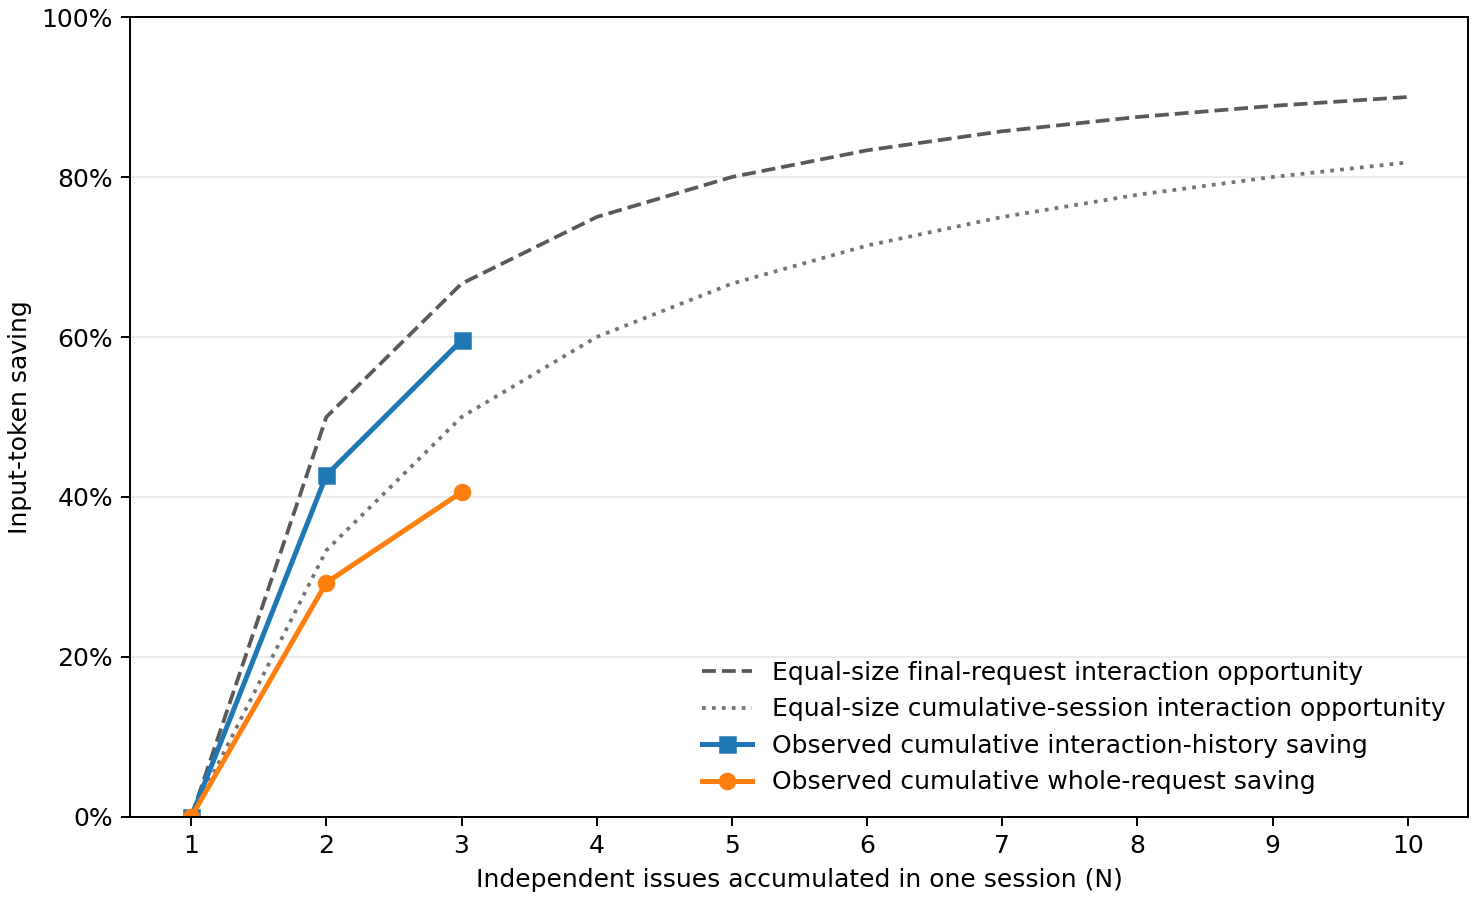
\includegraphics[width=.88\linewidth]{../shared/results/paper8_5_agent_memory/instruction_epoch_oracle_n3_clean_full_v1/instruction_epoch_scaling.png}
\caption{Instruction-epoch opportunity and observed saving as independent
issues accumulate in one session.  Lines beyond $N=3$ are structural
equal-size opportunities, not autonomous quality measurements.}
\label{fig:editorial-instruction-epoch-scaling}
\end{figure}

\subsection{Recent Frontier discovery cohort}

Recent Frontier applies recent, mutation, verification, and protocol floors
over a continuous session without requiring an explicit task-boundary signal.
The strict same-prefix Task~3--5 cohort is the strongest current paired point.

The cohort preserves all three qualified paired successes and reduces aggregate
calls, but savings range from 11.52\% to 52.56\% within trajectory.  It is a
promotion candidate, not evidence of greater-than-90\% population preservation
or a universal default.

\subsection{Prompt Pinned discovery cohort}

Prompt Pinned preserves every genuine user prompt, the active instruction
epoch, the two most recent completed epochs, and compact closure evidence for
older completed epochs.  Cold exact-prefix execution removes a cache-state
confound and yields one task-clustered observation per identity.

Prompt Pinned is conceptually distinct from Recent Frontier and reaches the
30--50\% target band on this small cohort.  Its closure receipts are
model-visible post-cache transformations in the current transfer experiments.
Two direct-host selection-only E2 executions, including one cold model reload,
repeat exactly and preserve 2/2 official solves on one identity at 40.56\%
own-trajectory saving without synthetic receipts.  This qualifies strict
repeatability for one task; additional identities remain necessary before
recommendation as a native-PRA default.

\subsection{Post-refactor matched-recency audit}

An implementation audit found that the historical matched-tail manifests
recorded two protected head and four protected tail turns although the
materializer consumed neither parameter.  Re-reducing the immutable artifacts
reproduces every archived total, and four fresh Task~2--3 \textsc{Full}
controls reproduce their old official outcomes, calls, and cumulative tokens
exactly.  The refactor therefore did not alter the baseline or reducer; the
historical treatment is a valid prompt-pinned pure-recency policy with a
superseded H2/T4 label.

The corrected H2/T4 arm keeps the first two and latest four complete causal
turns.  On the same three identities it preserves 3/3 official resolutions,
but uses 64 calls versus 61/69 for FULL-A/FULL-B.  It saves 6.03\% through
whole-causal-group retirement and 8.17\% after record-internal span
materialization against its own trajectory counterfactual, plus 6.28\%
against pooled FULL-A input; the
task-macro paired value is $-3.93$\% because Task~2 expands from 15 to 22
calls.  Thus corrected H2/T4 passes the observed quality gate but fails the
predeclared no-call-increase efficiency gate.  A second corrected Task~1 run
also resolves, but uses 26 rather than 20 calls, exposing residual trajectory
variance.  Neither corrected nor legacy matched recency is promoted as a
default.

The corrected OpenHands transfer supplies a useful contrast without changing
the selector.  OpenHands 1.49.2 on Tasks~1--3 resolves 3/3 officially and uses
74 rather than 77 actions.  Task~1 emits the same 689-byte patch digest as its
paired successful \textsc{Full} control and saves 35.35\% against its own
logical history and 43.53\% against paired \textsc{Full}.  Task~2 produces a
different but resolving patch, saves 9.12\% against its own counterfactual and
6.12\% paired, and adds one action.  Task~3 also resolves with a semantically
equivalent patch, uses 17 versus 19 actions, and saves 8.14\% own and 18.75\%
paired.  Aggregated over task identities, H2/T4 saves 22.67\% own and 29.76\%
paired input.  The 8.14--35.35\% range arises
because Task~1 contains an oversized early source view that can retire once
more specific reads supersede it.  This three-identity result is not a population
accuracy estimate, but it demonstrates that the corrected policy is transverse
to the agent interface and that opportunity is workload-dependent.

The next exact transfer prevents a favorable-only interpretation.  Pi 0.75.3
solves the same task under a fresh 28-call \textsc{Full} control, but corrected
H2/T4 fails in 28 calls.  It saves 8.53\% of materialized ordinary-text input
while retiring only 0.30\% as whole causal groups.  The first changed input
precedes the first changed tool action; after repeated edit failures the agent
copies a partial fragment over a complete source file, producing a 91,283-byte
patch that fails the official grader.  The apparent saving mostly comes from
rewriting one selected oversized source view, not omitting reusable records.
We therefore supersede generic boundary rewriting with a declared-safe rule:
an observation may be subdivided only into stable natural child spans created
before model-visible materialization and K/V encoding.  Otherwise the policy
retires the whole causal group or leaves budget unused.  This negative result
is a policy-transfer failure, not an inference-engine result.

The repaired Pi reruns validate that distinction.  Declared-safe H2/T4 and
H2/T8 both resolve officially and reproduce the FULL control's exact 689-byte
patch digest.  H2/T4 saves 45.16\% against its own whole-record counterfactual
but expands to 43 model calls and saves only 1.40\% against paired FULL input.
The predeclared H2/T8 mitigation reduces the expansion to 39 calls, saves
41.53\% within trajectory and 11.81\% against paired FULL, but still fails the
no-call-increase and paired-economics gates.  Its first 13 actions match FULL;
the first divergence follows selection at request~13 and a third schema-invalid
edit result.  Thus the unsafe rewrite was a real correctness bug, while the
remaining inefficiency is an agent recovery/conditioning result requiring
causal add-back rather than a wider tail-size grid.

The first normalized Kilo pairing adds a complementary negative result.  Kilo
injects a wall-clock \texttt{Message time} field into the model-visible user
record; a generic request-normalization declaration replaces only that
volatile field before both hashing and forwarding.  The resulting Full and
declared-safe H2/T4 arms have the same initial request digest and generation
controls, resolve officially, and emit the same 689-byte patch.  Nevertheless,
their first canonical tool actions differ at action~1, seven requests before
selection first changes an input.  The candidate saves 7.30\% against its own
whole-record counterfactual but materializes 376,980 selected tokens versus
146,013 in Full, or $-158.18$\% paired saving.  We therefore reject causal
attribution and promotion: temperature zero and identical first inputs do not
guarantee a repeatable backend trajectory.

\subsection{Task-clustered headline comparison}

Table~\ref{tab:editorial-headline-policies} keeps discovery and confirmation
separate.  Matched Recency contains six executions over three identities and
is shown as a negative control; its historical schema lacks three immutable
pairing digests and is not pooled with the exact-prefix cohorts.  The frozen
Recent-Frontier held-out confirmation now completes all eight predeclared
identities under the baseline-conditional missingness rule.  Prompt Pinned's
separate held-out arm remains at its first independently cold identity; its
same-prefix \textsc{Full} repeat fails identically and therefore launches no
treatment.

\begin{table}[H]
\centering
\scriptsize
\setlength{\tabcolsep}{3pt}
\begin{tabularx}{\linewidth}{p{.145\linewidth}p{.095\linewidth}p{.08\linewidth}p{.10\linewidth}p{.09\linewidth}p{.15\linewidth}p{.115\linewidth}Y}
\toprule
Policy & Cohort & IDs & Resolved F/P & Calls F/P & Input F/P & Save own/paired & Status \\
\midrule
Matched Recency & development & 3 (6 runs) & 5/6; 4/6 & 154/113 & not admitted & 6.35\%/n.a. & two losses; incomplete legacy identity \\
Matched Recency H2/T4 & post-fix audit & 3 & 3/3; 3/3 & 61/64 & 364,457/341,556 & 6.03L/8.17M; 6.28P\% & $+3$ calls; not promoted \\
Matched Recency H2/T4 & OpenHands post-fix & 3 & 3/3; 3/3 & 77/74 & 932,038/654,626 & 22.67/29.76\% & $-3$ actions; three-task transfer \\
Matched Recency H2/T4 & Pi post-fix & 1 & 1/1; 0/1 & 28/28 & 464,135/424,805 & 0.30L/8.53M; 8.47P\% & lost success; superseded \\
Declared-safe H2/T8 & Pi repair audit & 1 & 1/1; 1/1 & 28/39 & 464,135/409,335 & 41.53/11.81\% & same patch; $+11$ calls \\
Declared-safe H2/T4 & Kilo pairing audit & 1 & 1/1; 1/1 & 20/19 & 146,013/376,980 & 7.30/$-158.2$\% & preselection fork; noncausal \\
Recent Frontier M2/P1 & OpenHands single epoch & 1 & 1/1; 1/1 & 25/33 & 186,635/287,257 & 0.00/$-53.91$\% & exact abstention; divergence before selection \\
Recent Frontier M2/P1 & development & 3 & 3/3 & 30/22 & 556,072/239,881 & 40.53/56.86\% & calls decrease \\
Prompt Pinned E2+F1C & development & 3 & 3/3 & 34/33 & 924,686/539,022 & 39.45/41.71\% & transformed receipts \\
Recent Frontier M2/P1 & held-out & 8 & 3/8; 3/3 elig. & 37/37 elig. & 829,884/497,538 elig. & 15.59/40.05\% & no eligible loss; Full only 3/8 \\
Recent Frontier M2/P1 & held-out order 2 & 8 & 1/8; 1/1 elig. & 27/27 elig. & 153,654/153,654 elig. & n.a./0.00\% & exact abstention; Full only 1/8 \\
Prompt Pinned E2+F1C & held-out & 1/8 & 0/1; --- & 14/--- & 97,604/--- & --- & Full failed; no candidate \\
\bottomrule
\end{tabularx}
\caption{Task-clustered policy ledger at cutoff.  F/P denotes Full/policy.
Discovery and held-out confirmation are never aggregated; repeated runs expose
instability but do not increase the identity denominator.  For the completed
Recent-Frontier row, ``elig.'' conditions policy accuracy and paired saving on
the three identities solved by contemporaneous exact-prefix \textsc{Full};
15.59\% is the unconditional whole-session saving after carrying five failed
\textsc{Full} episodes.  The second order has one qualified eligible identity
and seven failed controls; its only admitted policy arm abstains at 0\% saving,
so no unconditional saving is reported.}
\label{tab:editorial-headline-policies}
\end{table}

The OpenHands single-epoch row is deliberately a scope and variance control,
not a failed saving policy.  With only one visible user instruction, the last
$M=2$ instruction frontier contains the entire session, so M2/P1 has no older
epoch eligible for retirement.  Its 0\% own saving is exact.  The 53.91\%
paired cost increase follows a response-9 fork under identical selected
message content and therefore cannot be attributed to selection.  This
control prevents the persistent-session policy from being misreported as a
single-task compressor and reinforces task-clustered repeat controls.

The held-out rows make the uncertainty visible rather than inflating the
denominator.  In the first order, exact-prefix \textsc{Full} resolves only 3/8
identities; M2/P1 preserves all three eligible successes and their aggregate
37-call workload while reducing paired input by 40.05\%.  Carrying the five
failed \textsc{Full} episodes through the same persistent session reduces the
unconditional saving to 15.59\%.  In the reversed order, \textsc{Full} resolves
only 1/8 and the sole eligible M2/P1 arm is an exact 0\%-saving abstention.
These observations qualify a mechanism on three first-order paired successes,
not a population preservation rate.

Diagnostics on failed controls are likewise kept out of the preservation
denominator.  The normalized first order recovers one cross-task failure, but
the reversed order recovers 0/6 while omitting 48.98\% of candidate-own input
and increasing calls from 92 to 104.  Thus old-task interference sometimes
matters, but recovery is prefix- and order-sensitive and does not explain the
cohort generally.  Appendix~\ref{sec:detailed-evidence-ledger} retains the task
order, runtime normalization, submission analysis, and complete failure
ledgers.

\begin{figure}[H]
\centering
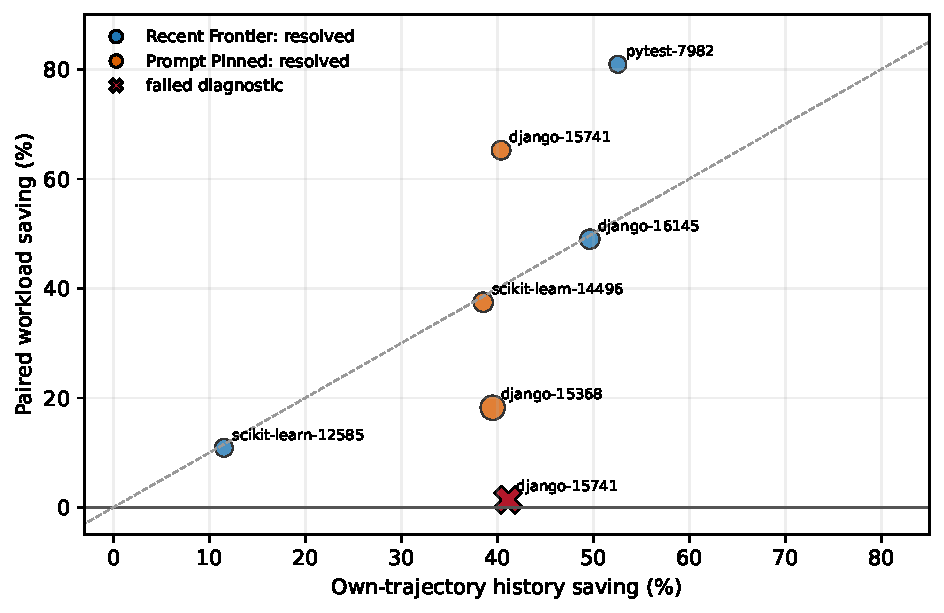
\includegraphics[width=.80\linewidth]{../shared/results/paper8_5_agent_memory/v2_trajectory_economics/trajectory_economics.pdf}
\caption{Own-trajectory omission versus paired workload saving.  Marker area is
proportional to policy calls; filled circles preserve the paired official solve
and the cross marks the failed Recent-Frontier diagnostic.  High omission can
collapse after trajectory inflation.}
\label{fig:trajectory-economics}
\end{figure}

\section{Profile Implications}

The evidence supports a staged candidate vocabulary, not one universally best
selector.  Candidates differ in how much uncertainty they tolerate and in
which evidence floors they preserve.  Table~\ref{tab:profile-implications}
separates frozen discovery points from controls and unqualified treatments.

\begin{table}[H]
\centering
\small
\begin{tabularx}{\linewidth}{p{.16\linewidth}p{.24\linewidth}p{.28\linewidth}Y}
\toprule
Profile & Logical policy & Non-negotiable state & Current evidence \\
\midrule
Exact & Full history & all canonical records & control and repeatability baseline \\
Conservative & wide Recent Frontier & prompts, current turn, recent mutation/verification/protocol spine & bounds session growth; parameters require workload gate \\
Balanced candidate & repeat-qualified Recent Frontier (M2/P1) & same floors with bounded older causal groups & 3/3 paired discovery plus 3/3 eligible first-order held-out successes; second order has one exact 0\%-saving eligible control and 0/6 failed-Full recoveries \\
Experimental economy & Prompt Pinned (E2+F1C) & all prompts, active/recent epochs, closure evidence & 3/3 cold identities; hybrid receipts prevent strict native promotion \\
\bottomrule
\end{tabularx}
\caption{Evidence-based profile interpretation.  Names express operating
intent; they do not convert discovery cohorts into population guarantees.}
\label{tab:profile-implications}
\end{table}

Promotion requires a larger held-out task cohort, repeat runs clustered by task,
another model family, and another agent harness.  The same selector must also be
tested in both one-task-per-session and persistent multi-task modes.  A policy
that helps only after explicit task segmentation is not a general session-memory
policy; a policy that retains all prior independent issues cannot deliver the
asymptotic benefit that motivates native addressable K/V.

The practical default-selection rule is correspondingly simple: prefer the
least aggressive profile that meets the application's memory bound, and fall
back toward Full when dependency evidence, protocol state, or model behavior is
uncertain.  Savings are accepted only when official resolution is preserved on
the paired eligible cohort and aggregate calls do not increase.  This rule
turns the paper's negative results into an operational guardrail rather than a
claim that all semantic selection is unsafe.

\section{Frozen Runtime Handoff}

Paper~8.5 freezes record identities, spans, original positions, replacements,
and a plan digest.  It does not infer engine performance from logical tokens.
For a selection-only plan, the cumulative selected original-token count is the
engine-independent upper bound on reusable K/V demand.  Paper~4.5 must replay
the identical ledger and report page rounding, resident references, physical
copies, newly evaluated suffix tokens, and temporary bytes separately.  A
logical saving difference across engines is a failed ledger comparison, not an
engine result.

Earlier runtime-transfer diagnostics preceded the current engine fixes and are
not used as post-fix evidence here.  They also mixed strict selection with
model-visible closure receipts.  A receipt created after source K/V exists is
transformed context: its tokens require evaluation and cannot be credited as
native reuse.  The post-fix Paper~4.5 handoff will therefore map only frozen
selection-only plans directly to K/V omission; ingest-time compaction and
post-cache transformation remain separate treatments.

\section{Discussion and Limitations}

\paragraph{What the positive points establish.}
Recent Frontier and Prompt Pinned are two independently motivated mechanisms
that cross the intended 30--50\% logical-saving band on small qualified
cohorts while preserving their paired successes.  They show that useful agent
history is not synonymous with a blind suffix and that substantial removable
history can exist without an explicit task-boundary signal.  They do not yet
estimate population accuracy, establish a production default, or show that the
same parameters transfer unchanged across agents and models.

\paragraph{What the negative points establish.}
Whole-record semantic deletion fails for a deeper reason than an unfortunate
threshold: current-world authority and reasoning utility have different
lifetimes.  Likewise, a low per-request retention ratio can be economically
negative when it causes recovery.  These observations constrain future policy
design: use negative selection conservatively, retain protocol and mutation
floors, and promote policies on paired cumulative work rather than on nominal
token omission.

\paragraph{Oracle scope.}
Leave-one-bundle-out and bounded subset search answer whether headroom exists
on a frozen successful trajectory.  They cannot predict the new trajectory
created by omission, and independent removability does not imply joint
removability.  Oracle results are therefore hypothesis generators and add-back
diagnostics, not deployable policies or accuracy estimates.

\paragraph{External validity.}
The autonomous evidence uses mini-swe-agent, a Bash tool surface, a small number
of SWE-bench Verified identities, and primarily Qwen3-Coder-30B.  Bash is useful
because file reads, writes, searches, tests, and return codes can be typed from
commands and observations.  Controlled Pi, Kilo, and PRA-Agent admissions now
establish that two native typed-tool protocols and one record-native agent all
solve the same locked task under exact \textsc{Full} controls.  These are
compatibility results, not policy-accuracy estimates: future work must still
reproduce the savings findings across the locked cohort, then cover a current
richer open-agent runtime, another model family, longer dependent sessions,
and task-clustered confidence intervals.

\paragraph{Runtime boundary.}
Logical omission says which existing records a model should see.  It does not
say whether an engine re-encodes text, copies K/V, preserves original
positions, or creates large temporaries.  Post-cache receipts also introduce
new tokens and must be charged.  Paper~4.5 receives the frozen plan and owns
those physical and numerical gates.

\section{Conclusion}

Agent history is not a bag of tokens and not merely a snapshot of current world
state.  Provenance, control, and semantic evidence can outlive the state they
helped create.  Whole-record deletion is consequently an unreliable abstraction.
Structured boundary-free policies expose meaningful removable-history
opportunity on repeat-qualified SWE-bench tasks, but the current cohorts are
small and heterogeneous.  The defensible endpoint is trajectory economics:
official resolution, reacquisition, calls, and cumulative work, not a nominal
retention percentage.  Logical policy and physical runtime realization remain
separate contracts.

\clearpage
\appendix
\section{Detailed Methods and Evidence Ledger}
\label{sec:detailed-evidence-ledger}

The remainder preserves the full policy-development chronology, rejected
variants, oracle grids, infrastructure quarantines, and artifact paths for
auditability.  These details are not additional main-paper claims.

\section{Background and Motivation}

\subsection{Agent history differs from document retrieval}

Document retrieval typically selects evidence that is externally stored and
largely immutable. Agent memory contains generated and observed state whose
meaning depends on the trajectory. A source observation may explain a later
edit; an edit invalidates earlier verification; a rejected action may produce
an error observation without becoming part of the accepted action history.

These dependencies motivate a record graph rather than an undifferentiated
token stream.

\subsection{Why mini-swe-agent}

mini-swe-agent maintains a linear message list. At each step the model receives
that list, returns one or more actions, the environment executes those actions,
and formatted observations are appended. Because there is little additional
memory management in the harness, the trajectory itself is the natural object
for intervention.

We use mini-swe-agent as the first experimental harness, then test whether the
highest-performing policies transfer to a richer open-source agent and to a
record-native PRA agent.

mini-swe-agent exposes one generic Bash action interface. Consequently, tool
choice is not a meaningful routing variable in this first study: the scientific
variables are which action--observation history survives and how large tool
observations are represented. We do not place a PRA gateway in the primary
factorial. Gateway tool routing and result compaction are separate interventions
that can be tested only after the logical memory policy is fixed.

\section{Agent Record Model}

We normalize trajectory messages into typed records:
\[
\begin{aligned}
\mathcal R = \{&\textsc{Task},\textsc{Action},\textsc{Observation},
\textsc{Source},\textsc{Mutation},\\
&\textsc{Verification},\textsc{Progress},\textsc{Error},
\textsc{Finalization}\}.
\end{aligned}
\]

Each record contains a stable identifier, turn index, semantic type, causal
group, source identity/spans where applicable, mutation target, and logical
creation time.

\subsection{State, provenance, control, and semantic utility}

A record has several lifetimes rather than one scalar relevance value. For a
record $r$ at decision $t$, we use the conceptual decomposition
\[
U(r,t)=U_{\mathrm{state}}(r,t)+U_{\mathrm{provenance}}(r,t)
      +U_{\mathrm{control}}(r,t)+U_{\mathrm{semantic}}(r,t).
\]
$U_{\mathrm{state}}$ measures whether the payload authoritatively describes
the current external world, such as a file at a particular version.
$U_{\mathrm{provenance}}$ records why the agent inspected or changed that
resource. $U_{\mathrm{control}}$ carries progress, hypotheses, intended next
steps, and finalization state. $U_{\mathrm{semantic}}$ captures facts useful
for later reasoning even when they are no longer the current-state projection,
such as an old traceback that exposes an architectural constraint.

The DAG can sometimes establish that a payload is operationally superseded,
but this proves only a reduction in $U_{\mathrm{state}}$. In particular,
\[
\text{state superseded}\ \not\Rightarrow\ \text{record behaviorally useless}.
\]
This distinction motivates partial retirement: retain action/provenance and a
typed state transition while eliding replaceable bulk payload. It also
explains why operational certificates and behavioral outcomes are separate
measurements throughout the paper.

\subsection{Causal bundles}

Actions and observations are grouped:
\[
\textsc{Action}_i \leftrightarrow \textsc{Observation}_i.
\]
Mutations and later verification can form a higher-level dependency:
\[
\textsc{Mutation}_i \rightarrow \textsc{Verification}_j.
\]

Policies may rank individual records, but required bundles are rounded up unless
the experiment explicitly tests bundle-breaking.

\section{Memory Selection Policies}

\subsection{Full history}

\textbf{FULL} retains all canonical records and defines the reference trajectory.

\subsection{Recency baselines}

We test:
\begin{itemize}[leftmargin=*]
    \item \textbf{TOKEN-TAIL}: last $B$ tokens;
    \item \textbf{TURN-TAIL}: last $N$ complete turns;
    \item \textbf{RECORD-TAIL}: last $M$ records;
    \item \textbf{CAUSAL-TAIL}: last $N$ complete causal bundles.
\end{itemize}

\subsection{Independent head, middle, and tail}

Recency and early-run retention are separate variables. We therefore define a
three-zone policy
\[
S_t = I \cup H_h \cup \pi_{\mathrm{middle}}(M_t,Q_t,B') \cup T_\tau,
\]
where $I$ is the immutable system prompt and all user-authored instructions,
$H_h$ contains the
first $h$ complete action--observation turns, $T_\tau$ contains the latest
$\tau$ complete turns, and the selector operates only on the non-overlapping
middle $M_t$. The head and tail controls are independent; $h=0$ never removes
$I$.  Thus task definitions and later user prompts are not optimization
candidates in this study.  A tool observation transported through a
user-role message remains selectable because its semantic type and provenance
are \textsc{Tool-Observation}, not \textsc{User-Instruction}.  Oversized user
instructions may eventually be handled internally by an engine-side PRA
implementation, but that is outside the logical-retirement intervention
measured here. Our pilot grid uses
\[
h\in\{0,1,2,4\},\qquad \tau\in\{1,2,3,5,10\}.
\]
Frozen replay eliminates dominated combinations before autonomous evaluation.
This factorization tests whether early localization or plan formation remains
useful after leaving a conventional recency window.

Head and tail turns remain causally complete. An oversized tool observation is
the only permitted within-turn exception: its action, return code, resource
identity, mutation/verification status, error headline, and causal identity
remain present while its body may use a separately recorded detail policy.
When immutable/head/tail state exceeds the requested budget, we report
mandatory overflow and realized retention rather than silently breaking a turn.

\subsection{Typed progress spine}

The structured policy retains
\[
S_{\mathrm{spine}} =
T
\cup
R_{\mathrm{recent}}
\cup
S_{\mathrm{source}}
\cup
M_{\mathrm{mutation}}
\cup
V_{\mathrm{verification}}
\cup
P_{\mathrm{progress}},
\]
where each component denotes the latest required records of that semantic role.

\subsection{Persistent multi-issue sessions}

A developer may solve several issues without opening a new conversation.  We
therefore separate the issue from the session: an \emph{episode} is one issue
and workspace lifetime, while a session is an ordered sequence of one or more
episodes.  Two modes consume the identical locked issue order:
\textsc{Fresh-Per-Issue} assigns a new session identity to every episode, and
\textsc{Persistent} retains one identity across $n\in\{1,2,3,4,5\}$ episodes.
Every transition declares the new active task, workspace scope, prior episode
completion, and globally unique record, turn, and causal-group identities.
Incompatible SWE-bench base commits remain separate workspaces; persistent
conversation state must not be confused with a physically merged repository.

The first episode-aware policy keeps the active episode whole and retains each
completed episode's task statement, newest complete turn, latest mutation, and
latest verification.  An early aggressive diagnostic kept only the system
prompt and active episode.  That legacy arm is now superseded because it could
remove an earlier user-authored task statement.  Under the current invariant,
``active only'' can retire all completed assistant--tool interaction but still
retains every user instruction.  These episode policies operate before any within-episode token budget, so their
saving can grow with the number of completed issues instead of being capped by
a nominal 90\% retention treatment.

Explicit episode boundaries are useful to an evaluator but are not a sound
deployment assumption: developers need not announce that a new issue has
started.  We therefore also evaluate a \emph{boundary-free global} policy over
one continuous transcript.  It receives no episode identifier, completion
marker, or workspace-scope annotation.  Every user-authored instruction is
still immutable, while recent-turn, mutation, verification, and protocol
floors are computed globally over typed assistant--tool causal groups.  This
arm isolates the realistic question: how much of the tool-interaction history
can be retired when the selector is not told where one task ends and another
begins?

\subsection{Retrieval policies}

We compare lexical, dense, and hybrid retrieval over historical records using a
query formed from
\[
\text{task}
+
\text{current progress}
+
\text{latest active observation}.
\]

The hybrid policy combines a mandatory structured spine with retrieved records.

\subsection{Resource/effect DAG and negative exclusion}

Positive selection asks which records are likely useful. We additionally test
the dual question: which records are operationally obsolete under a declared
resource-state abstraction? We construct an acyclic graph over actions,
observations, immutable resource versions, and precisely defined projections.
Typed edges include \textsc{Returns}, \textsc{ReadsFrom}, \textsc{Writes},
\textsc{SupersededBy}, and \textsc{SubsumedBy}. Effects carry provenance from
declared tool semantics, runtime tracing, static heuristics, or \textsc{Unknown};
unknown effects prohibit certified exclusion.

The two-stage policy is
\[
H_t \xrightarrow{\text{certified exclusion}} H'_t
\xrightarrow[\text{only if still over }B]{\pi_{\mathrm{positive}}} S_t.
\]
A certificate names the rule, witnesses, proof scope, resource-version
fingerprints, cwd/environment identity, completeness conditions, and explicit
assumptions. We separate three tiers: \textsc{Dag-Certified},
\textsc{Dag-Recoverable}, and \textsc{Dag-Heuristic}. Only the first is removed
by the conservative $B=100\%$ exclusion arm; the others require the same
counterfactual and autonomous qualification as positive retrieval.

The scope of ``certified'' is deliberately narrow. A later record can be proven
to supersede an older current-state projection, but this does not prove that the
older text contains no decision-relevant diagnostic fact. Moreover, deleting
even byte-identical repeated text changes token positions and attention. Thus
the claimed property is \emph{certificate-backed operational obsolescence},
not risk-free behavioral equivalence. Behavioral preservation remains an
empirical outcome measured by frozen replay and autonomous tasks.

The initial executable rule, \textsc{Trace-Exact-Operation-Result}, compares the
executed command and complete observation rather than the assistant's private
reasoning prose.  It fires only when cwd, environment identity, affected
resource-version fingerprints, return code, and observation bytes agree under
runtime-traced or declared-complete semantics.  The older whole causal bundle
is then operationally redundant.  Different reasoning prose is intentionally
outside the certificate, which is why frozen behavioral qualification remains
required even for this strongest exclusion tier.

Initial rules fail closed: system/task/current state and unresolved errors are
protected; arbitrary or untraced Bash is \textsc{Unknown}; output must be
complete and non-truncated; file reads require canonical paths and version/span
identity; git queries require separate HEAD, index, and worktree identities;
and action--observation bundles remain intact. A write invalidates an old record
as an authority on current state but does not by itself authorize semantic
deletion. Similarly, a later passing test does not automatically erase a prior
failure's diagnostic information.

\subsubsection{Auditable negative-selection heuristic ladder}

Certification coverage will initially be sparse, so we test four explicitly
non-certified negative-selection families before invoking learned relevance.
All retire complete action--observation groups, preserve independent head and
tail floors, and emit a compact inactive tombstone containing the rule,
resource, and witness identities. The tombstone is controller provenance and
is not serialized into the model request; serializing it would be a distinct
summarization treatment.

\textsc{H1--Consumed Search} retires a discovery operation such as
\texttt{find}, \texttt{fd}, \texttt{rg --files}, or filename-only
\texttt{grep -l} after a returned resource is consumed by a concrete source
read and the trajectory subsequently advances to a non-read operation.
Source-bearing \texttt{grep -n} and ordinary \texttt{rg} matches count as
reads, not discovery. The delay $K_f\in\{0,1,2,4\}$ starts at that transition
and measures whether the location evidence retains short-lived value after
consumption. An unresolved search/read exploration chain is not retired.

\textsc{H2--Write Consolidation} is split because absence of a rewrite does
not imply that a mutation was good. H2a requires an observed resource change
and a later read or diff of the same post-write version. H2b requires a
successful verification with an explicit dependency on the written resource;
a workspace-wide passing check is a separately labelled relaxed arm. Only the
raw write bundle is retired, while the later current-state or verification
evidence remains. The bare ``no later rewrite'' rule is retained solely as an
aggressive ablation with $K_w\in\{1,2,4\}$.

\textsc{H3--Read Supersession} retains the latest $K_r$ observations, for
$K_r\in\{1,2,3\}$, covering each resource--version--span key. A whole-file
read covers a line span; a later disjoint \texttt{sed} region does not;
grep/tail projections require the same query signature. Missing versions use a
no-intervening-write epoch only in the heuristic tier and never become a
certificate.

\textsc{H4--Bounded Working Set} retains the latest
$K_x\in\{2,3,4,6\}$ distinct read resources while pinning resources named by
the task, mutated state, unresolved failures, the current tail, and declared
dependencies. Cross-file software dependencies make H4 the riskiest family;
it is reported as a capacity heuristic rather than safe exclusion.

The initial grids above target short trajectories.  We separately predeclare
a long-horizon grid with $K_f\in\{0,2,4,8,12,16\}$,
$K_w\in\{1,2,4,8,12\}$, $K_r\in\{1,2,3,4,6,8\}$, and
$K_x\in\{2,3,4,6,8,12\}$.  Its primary cohort contains only ordinary
\textsc{Full} executions that resolve officially, contain at least 25 model
decisions, and exceed 100,000 cumulative exact-tokenizer input tokens.  We
report both the complete growing-prefix integral and suffixes beginning at
decisions 10, 15, and 20.  This tests a specific nonstationarity hypothesis:
after workspace mutations, old observations may cease to be authoritative
even though task intent, mutation rationale, and unresolved failures can
remain useful.  Age alone is therefore never treated as evidence of
irrelevance.

The high-retention sweep uses targets 100\%, 99\%, 97.5\%, 95\%, and 90\%.
Every semantic arm is paired with a recency control using its exact
per-decision materialized-token count; a fixed keep-last-$K$ control is also
reported to show how its realized retention changes with task length.  This
matched design asks whether resource/version/effect evidence removes stale
state more efficiently than blind age, rather than merely comparing policies
that remove different numbers of tokens.

The predeclared sequence isolates H1, H2a, H2b, H3, and H4 before combining
H1+H3, H2+H3, H1+H2+H3, and finally all four. If the negative stage remains
over budget, the original absolute budget is passed to the positive selector.
This ordering identifies whether failure came from a particular retirement
rule or from subsequent relevance selection.

\subsubsection{Tool-semantics ownership and runtime handoff}

mini-swe-agent exposes only one generic Bash tool, so the Paper~8.5 harness
provides a Bash-specific semantics adapter that classifies common commands and,
when available, augments them with runtime filesystem/version tracing. This
special case belongs in the harness-facing adapter, not in a PRA inference
engine. The first implementation certifies only simple allowlisted read or pure
commands. Pipelines, lists, substitutions, redirections, heredocs, multiline
scripts, timeouts, and truncated observations fail closed even when a coarse
regex suggests a familiar command category.

The instrumented Docker environment leaves the model-visible observation text
unchanged and attaches a versioned metadata envelope containing canonical cwd,
environment identity, return and completeness status, pre/post resource
fingerprints, and pre/post repository-state fingerprints. Before every action
it also stores the base commit, separate binary index and worktree patches, and
an archive of nonignored untracked files. Untracked file contents, not only
their names, participate in the state digest. This is an exact, restorable
repository state under the declared scope; ignored artifacts, container-global
state, network state, and resources outside the repository remain explicitly
out of scope. A restore verifier refuses incomplete receipts, dirty targets,
digest mismatches, and unsafe archive paths.

The portable interface is instead a tool-semantics provider. A developer or
agent SDK can declare generic reads, writes, deletes, verification targets,
resource versions, causal dependencies, output completeness, and confidence.
The contract separates transport status, semantic outcome, result completeness,
and effect-trace completeness.  Therefore an HTTP-complete or provider-stopped
exchange cannot masquerade as a successful tool operation or completed agent
task.  Failed action, error observation, and the dependent recovery are linked
as an atomic selection closure.  Thread, subagent, and parent-thread identities
support hierarchical agents without flattening private child histories into the
parent context.
It may also attach record directives such as protected, certified-excludable,
or preferred-for-selection, with a certificate and witness IDs. Future tool
categories implement the same effect vocabulary without teaching the engine
about Bash, Excel, browsers, databases, or particular agent frameworks.

The implementation now has a shared mediation layer that can run inside a PRA
runtime or, only when the engine cannot host it, in the external gateway. Both
placements consume the same content-addressed
\texttt{WireAgent\-Memory\-Plan}; stale-history digests and conflicting second-hop
mediation fail closed. Thus moving an unchanged plan between placements is a
conformance test, not a reason to rerun the entire policy campaign.

The common state-authority planner consumes only declared operation classes,
resource evidence (identity, version, and span), output completeness, and causal identities. It
contains no mini-swe-agent or Bash parser. The mini-swe-specific compatibility
code is confined to the evaluation adapter that translates its nonstandard
assistant--user Bash exchange to this portable schema. Standard typed tool
traffic, or an agent SDK that emits the schema directly, bypasses that adapter.
An embedded runtime supplies the exact model tokenizer for receipt size gates;
an external fallback must load the same tokenizer or consume an already frozen
plan.

When the policy returns to Paper~4.5, the PRA engine validates and physically
realizes selected logical identities; it does not infer application-specific
semantics. Paper~8.5 freezes selected IDs, replacement bytes, and a transfer-
admissibility label.  A selection-only plan is directly admissible to strict
native PRA.  A replacement created before initial cache admission is admissible
only as ingest-time compaction.  A replacement created after the source K/V
already exists is a transformed-context plan: Paper~4.5 must charge its model
evaluation and must not call it resident-subset reuse. Paper~4.5 then measures
cache hits, K/V movement, re-encoding, latency, memory, and lifecycle on those
same plans. Result compaction and tool disclosure are promoted independently
from shadow, so later gateway capabilities do not silently invalidate unchanged
history-policy evidence.

\subsection{Oracle}

A retrospective oracle estimates future usefulness through record/bundle
ablation on successful trajectories. It is an upper bound and is never used as
a deployment policy.

\section{Materialization Policies}

Record selection and record detail are separate variables.

For selected records, we compare:
\begin{itemize}[leftmargin=*]
    \item full record;
    \item matched source span;
    \item bounded head/tail;
    \item hierarchical child span;
    \item optional summary;
    \item compact provenance stub for an excluded record.
\end{itemize}

The first experiments use whole-record materialization so that selector effects
remain identifiable. A targeted second factorial applies detail reduction only
to oversized tool observations. Source views retain matched symbol/file spans;
test outputs retain the command, return code, failed-test identities, exception,
and relevant stack frames; search results retain matched lines and locations;
mutations retain their changed span or diff. This reuses gateway-style
compaction semantics without introducing a gateway or an engine into the study.

Negative exclusion therefore has two separately measured realizations. The
primary arm removes the retired payload from the model request while retaining
its tombstone only in controller state. A second \emph{model-visible stub} arm
replaces it with compact metadata such as resource, mutation/verification
status, and superseding-witness identity. The latter may preserve useful
provenance, but it is a materialization/compression treatment rather than pure
exclusion and its stub tokens count against the realized budget. This cleanly
separates binary HOT$\rightarrow$WARM retirement from
HOT$\rightarrow$STUB presentation.

For transfer we classify every treatment by when model-visible bytes are
created:
\begin{description}[leftmargin=!,labelwidth=3.4cm]
    \item[Selection-only.] Existing records are retained or omitted; the plan
    can be realized solely by selecting original resident K/V.
    \item[Ingest-time transform.] A tool result is compacted before its first
    model evaluation.  The compact form may subsequently acquire and reuse its
    own resident K/V, but it is not a transformation of existing K/V.
    \item[Post-cache transform.] Existing records are replaced with newly
    written summaries, tombstones, or receipts.  This requires new model
    evaluation and is not strict native PRA, even when every retained original
    record is reused without copying.
\end{description}
Accordingly, a compact receipt can improve logical task behavior while being
inadmissible to the strict resident-subset engine profile.  DAG evidence used
only by the selector remains out of band and adds no model tokens.

\section{Experimental Design}

\subsection{Recordizer reliability}

Policies cannot be credited for semantic types that the recordizer identifies
unreliably. We therefore separate tool-grounded labels (operation, resource,
version, return code, mutation, and verification) from prose-inferred labels
such as \textsc{Progress}. A blinded worksheet has now sampled 150 of 164
records from three frozen task trajectories, stratified by task, automatic
primary role, and early/middle/late trajectory position. It reports
per-type precision and recall plus exact causal-group boundary agreement.
Policy results expose both the declared/runtime-grounded view and the inferred
semantic view; low-precision inferred roles cannot support a default profile.
The worksheet and digest-bound source manifest are released under
\texttt{recordizer\_audit\_v1}; the present draft makes no reliability claim
until its human-label columns are complete.

\subsection{Phase I: frozen-trajectory screening}

We begin from successful full-history trajectories. At each historical model
call we restore the corresponding workspace, apply a candidate memory policy,
and query the same frozen model.

We measure:
\begin{itemize}[leftmargin=*]
    \item exact next-response agreement;
    \item exact action/command agreement;
    \item command equivalence under the frozen operation normalizer;
    \item target-resource agreement;
    \item semantic state-transition agreement (read, write, verification, or
    finalization with matching affected resources);
    \item final solution-state success for resumed rollouts;
    \item first-divergence turn;
    \item retained tokens and records.
\end{itemize}

Frozen screening permits broad policy and budget sweeps without paying for full
autonomous reruns.

The first frozen cohort follows a gate rather than a Cartesian sweep. On the
same instrumented successful trajectory, frozen model revision, tokenizer,
temperature zero, generation parameters, and decision snapshots, we run:

\begin{enumerate}[leftmargin=*]
    \item \textsc{Full}, establishing contemporaneous reproducibility;
    \item \textsc{Dag-Exclude} at a nominal 100\% ceiling;
    \item a recency/token-tail control matched to the DAG arm's realized token
    count at each decision;
    \item head--middle--tail policies at a 90\% minimum-retention floor,
    rounded upward at whole causal-turn boundaries.
\end{enumerate}

Failure of \textsc{Full} stops interpretation of later arms because it means the
frozen baseline itself was not reproduced. Autonomous qualification and oracle
add-back tests begin only after this ordered next-action gate. The matched-tail
control distinguishes the value of certified semantic exclusion from the value
of merely removing the same number of old tokens.

The two budget contracts are intentionally different.  The matched-tail arm
must not exceed the DAG arm's realized token count, so it rounds down and
reports unused capacity.  A treatment named ``90\%'', however, must retain at
least $\lceil0.9N\rceil$ logical tokens: it follows the policy ranking until the
next indivisible causal bundle crosses that floor and reports the resulting
whole-turn overshoot.  A preliminary implementation treated 90\% as a hard
ceiling and retained only 71.9\% on one decision; that partial run is
quarantined as a budget-contract failure rather than interpreted as policy
quality.

The repository state is part of the frozen decision point. Replaying turn $t$
restores the exact pre-action repository state within the declared checkpoint
scope, not merely the textual history, so a candidate command is evaluated
against the same tracked, staged, worktree, and nonignored-untracked contents as
the reference action.

\subsection{Phase II: autonomous evaluation}

Policies that survive frozen screening are run autonomously from a fresh task
sandbox. Final success is measured by the official SWE-bench grader.

Autonomous evaluation is required because a divergent action may still recover
later, while a seemingly small memory omission may cause many additional calls.

\subsection{Session schedule factorial}

For each promoted policy we run both \textsc{Fresh-Per-Issue} and
\textsc{Persistent} schedules over the same ordered issue sequences.  Required
controls are fresh \textsc{Full}, persistent \textsc{Full}, and persistent
policy selection.  Persistent \textsc{Full} can itself degrade through
cross-issue interference, so policy quality is compared both with its
contemporaneous persistent control and with official fresh-session resolution.
That whole-sequence control is necessary but not sufficient.  Once a treatment
changes an earlier trajectory, its next-task prefix differs from the separate
persistent-\textsc{Full} arm.  Before every persistent treatment episode, we
therefore run \textsc{Full} first from the treatment's exact serialized prefix,
with the same task, workspace snapshot, model, tokenizer, scaffold, and
generation settings.  The treatment is launched only if this in-place control
resolves officially.  If it fails, the cell is labelled
\texttt{unqualified\_session\_interference}; the heuristic is not launched and
the outcome is not counted as a heuristic failure.  Prefix and control hashes,
execution order, and official outcomes are retained in the ledger.
We report per-episode resolution, all-episodes resolution, calls, first
cross-issue contamination, current-prompt saving, and cumulative input saving.
The ordered issue sequence, not an individual request, is the uncertainty unit.
Paper~4.5 reuses the same schedule identifiers for K/V and runtime measurements.

\subsection{Benchmarks}

We begin with the existing SWE-bench Verified Easy-14 task sequence, then expand
to Easy-50 and a broader Verified sample.

Easy-14 is a mechanism/debug cohort. Publication-level claims require a larger
task set.

\subsection{Budgets}

We evaluate relative budgets
\[
100,\ 90,\ 75,\ 50,\ 25\%
\]
and absolute budgets
\[
2\mathrm K,\ 4\mathrm K,\ 8\mathrm K,\ 16\mathrm K,\ 32\mathrm K.
\]

Every request records both requested and realized retention.

\section{Metrics}

\subsection{Task outcome}

We retain official SWE-bench resolution as the primary benchmark endpoint, but
factor it into two separately reported agent outcomes:
\[
Y_{\mathrm{official}}=Y_{\mathrm{solve}}\land Y_{\mathrm{submit}}.
\]
$Y_{\mathrm{solve}}$ asks whether the final workspace contains a resolving
change; $Y_{\mathrm{submit}}$ asks whether the agent correctly emits that change
through the required terminal protocol. An auxiliary workspace grade can
identify $Y_{\mathrm{solve}}=1,Y_{\mathrm{submit}}=0$, but never replaces the
primary official result. If the final workspace cannot be reconstructed under
the fail-closed provenance rules, $Y_{\mathrm{solve}}$ is unknown rather than
zero. Additional endpoints are calls to completion, shell actions, and final
patch/test status.

\subsection{Memory efficiency}

We record full-history tokens, selected tokens, retention fraction, selected
record count, selected records by semantic role, and the largest retained
record.

For DAG policies we additionally report certified, recoverable, heuristic, and
unknown-effect tokens separately; certificate coverage and abstention; records
removed per rule; and certificate violations under frozen add-back tests. A
certificate can be operationally sound while the LLM still changes behavior,
so operational certificate validity and next-action survival are distinct
metrics.

We distinguish two savings quantities.  For an autonomous candidate trajectory
$c$, gross history saving is
\[
G_c=1-\frac{\sum_t M_{c,t}}{\sum_t F_{c,t}},
\]
where $M_{c,t}$ is materialized input and $F_{c,t}$ is the full-history
counterfactual at the same candidate call.  Gross saving isolates the memory
policy but does not charge for a longer trajectory.  Against a declared paired
\textsc{Full} execution $f$, paired trajectory message-input saving is
\[
N_{c,f}=1-\frac{\sum_t M_{c,t}}{\sum_t M_{f,t}}.
\]
$N$ includes extra or avoided calls, but covers only model-visible message
content. It excludes chat-template tokens, completions, tool execution, and
runtime; we therefore do not call it end-to-end saving. A failed run that
stops early can have a favorable $N$. For quality--efficiency frontiers we use
a failure-aware coordinate that charges an unsuccessful candidate at least
the paired \textsc{Full} message-input workload, so early failure cannot be
reported as an efficiency gain.

Direct recovery is also charged separately. Let $R_c$ be the token size of
tool observations produced by actions that reacquire previously excluded
resources. We report the diagnostic lower bound
\[
G^{\mathrm{reacq}}_c=
\frac{\sum_t(F_{c,t}-M_{c,t})-R_c}{\sum_tF_{c,t}}.
\]
This is not added to $N_{c,f}$: the paired trajectory quantity already includes
tokens replayed by a longer candidate trajectory. Instead, we expose recovery
as two complementary components,
\[
C_{\mathrm{recovery}}=C_{\mathrm{reacquire}}+C_{\mathrm{trajectory}},
\]
where the first is observed reread/search/test payload and the second is the
paired call and total-input-token inflation. Their overlap is reported rather
than summed into a potentially double-counted scalar.

\subsection{Quality--saving and interaction curves}

The primary frontier plots official task resolution against $G$ and $N$, with
$G^{\mathrm{reacq}}$ as a recovery-adjusted diagnostic.
Trajectory agreement is a diagnostic proxy, not accuracy: a different action
may still produce a resolving patch.  We therefore report separate curves for
(i) official resolution versus saving, (ii) tool-call delta versus saving over
all paired runs, (iii) tool-call delta restricted to pairs where both the
candidate and its declared \textsc{Full} control resolve, and (iv) first
tool-action divergence versus saving for every task. The divergence abscissa
uses only saving accumulated on requests strictly before the first different
action; tokens saved after divergence cannot explain that divergence and are
excluded from this plot.
Auxiliary terminal-workspace grading diagnoses submission failures but never
replaces official resolution.

Because the tested endpoint is not autonomously deterministic even at
temperature zero and a fixed seed, final quality curves use repeated paired
\textsc{Full} controls. Resolution is first averaged within task identity and
then across tasks; confidence intervals bootstrap task identities, never
individual executions. We report endpoint and exact-action agreement between
the \textsc{Full} repeats as an instability control. A conditional preservation
analysis additionally evaluates candidates only on declared pairs for which
\textsc{Full} resolves.  For multi-task treatment cells, the declared pair is
the successful in-place \textsc{Full} execution from the exact candidate prefix,
not merely an isolated-task success, an older run, or the divergent prefix of a
separate persistent-\textsc{Full} sequence.  This avoids treating session
interference or backend variability as a memory-policy failure while retaining
the unconditional resolution curve as a separate population result.

The current autonomous curve is deliberately underpowered and is reported as
a pilot, not a profile result. In the latest same-host three-task cohort,
repeated \textsc{Full} controls resolve 5/6 and matched recency resolves 4/6;
the latter misses the predeclared 80\% task-resolution gate. Earlier H3 runs
that failed early remain diagnostic points, but failure-aware saving assigns
them no efficiency gain. The manuscript therefore keeps raw gross saving,
paired trajectory saving, and qualification status as separate fields.

\subsection{Recovery behavior}

A memory policy may preserve final task success by forcing the agent to
reacquire forgotten state. We therefore count repeated source reads,
overlapping source rereads, repeated searches for the same fact, repeated tests
without relevant intervening mutation, and repeated failed edits. We call this
\emph{reacquisition overhead}.

For every negative arm we also report exclusions and tokens by rule, the
resource and witness provenance stored in inactive tombstones, and the fraction
of exclusions whose information is later reacquired. Frozen replay includes a
narrow immediate false-exclusion proxy: the selected-history generation reads
a hidden resource when contemporaneous \textsc{Full} does not. This proxy is
not a causal error rate---the primary evidence remains autonomous
reacquisition, calls-to-solution, and official task success.

\subsection{Dependency horizon}

For a useful historical record $r_i$ consumed at turn $t$, define
\[
d(r_i,t)=t-\operatorname{created}(r_i).
\]

We report dependency-age distributions by record type. This estimates how long
coding-agent memory must remain accessible.

\section{Main Results}

The central result is not that any old record can be deleted.  It is that a
policy needs an auditable unit of retirement.  Independent record deletion
breaks causal turns; keeping old user prompts while deleting their resolution
creates unanswered instructions; and retaining only current state removes
behavioral exemplars that condition valid tool use.  The safe unit found so
far is a terminally closed instruction epoch: its instruction and causal
interaction retire together, and only after a newer genuine user instruction
exists.  The selector receives no evaluator task identifier, workspace label,
or explicit issue boundary.

\begin{table}[H]
\centering
\scriptsize
\caption{Primary autonomous persistent-session frontier.  Easy-14 is one
ordered mechanism cohort.  Raw saving is cumulative selected message-content
input relative to paired \textsc{Full}; a lost paired success receives zero
failure-aware credit.}
\label{tab:main-frontier}
\begin{tabular}{>{\raggedright\arraybackslash}p{.22\linewidth}
                >{\centering\arraybackslash}p{.09\linewidth}
                >{\centering\arraybackslash}p{.12\linewidth}
                >{\centering\arraybackslash}p{.14\linewidth}
                >{\raggedright\arraybackslash}p{.26\linewidth}}
\toprule
Policy/cohort & Resolution & Calls & Saving & Interpretation \\
\midrule
Persistent \textsc{Full}, Easy-14 & 10/14 & 207 & 0\% & Context-qualified control; persistent history itself is not 14/14. \\
Atomic E2, stopped prefix & 2/5 vs 4/5 & 84 vs 85 & 28.22\% raw; 0\% failure-aware & Reject after two lost paired successes. \\
Atomic E3, Task-5 exact-prefix repeats & 1/2 vs 1/2 & 9 vs 8 & 16.62\% paired & Nondominated diagnostic, below target and adds one call. \\
Atomic E2, Task-5 exact-prefix repeats & 1/2 vs 1/2 & 27 vs 8 & $-106.77$\% paired & Reject: 41.94\% gross saving is erased by call inflation. \\
Atomic E2, earlier same-prefix diagnostic & 2/2 & 16,16 & 38.17\% own trajectory & Motivated confirmation but does not survive cross-task transfer. \\
Atomic active-only, one task & 0/1 & 22 & 71.03\% own trajectory & Reject: insufficient behavioral conditioning. \\
\bottomrule
\end{tabular}
\end{table}

The Easy-14 control changes the interpretation of the earlier single-task
positive.  The sequence comprises one continuous ordinary-role transcript over
fourteen clean official workspaces, with no evaluator issue identifier or
explicit boundary exposed to the policy.  \textsc{Full}'s 10/14 result is the
paired quality denominator, not the historical isolated-session 14/14 used to
select task identities.  Atomic E2 performs no retirement in Tasks~2--3, yet
the full-materialization repeats use 13 versus 18 and 19 versus 11 calls.
Selection begins at Task~4; E2 then loses the next two \textsc{Full} successes
through \texttt{patch\_apply\_failed}.  The arm is stopped rather than averaged
with nine unrun tasks.  Per-task traces, token denominators, and the failure
taxonomy are in the appendix.

E3 retains three complete prior epochs.  Its first four tasks are
full-materialization repeat controls and its first actual retirement is
Task~5.  The autonomous prefix diverges before that intervention: Tasks~3--4
both reach the 40-call limit despite \textsc{Full} using 11 and 23 calls.
We therefore stop that arm and fork Task~5 from the exact saved four-episode
\textsc{Full} prefix.  Across two executions, \textsc{Full}, E3, and E2 each
resolve 1/2.  E3 is the nondominated candidate but reaches only 16.62\% paired
saving and uses nine calls versus eight; E2 reaches the desired gross-retention
band but uses 27 calls and 106.77\% more paired tokens.  Promotion still
requires the complete fourteen-task sequence, no lost selection-active
\textsc{Full} success, no aggregate call increase, and a repeat of the selected
winner.  This design prevents raw token saving, early termination, or endpoint
variance from being mistaken for deployable utility.

The next policy revision replaces fixed epoch retirement with a forward
information-flow test.  Every genuine user message starts an instruction
epoch, the last $M$ prompts define a live frontier, and an older causal group is
eligible only when no path through instruction control, action--observation,
next-decision, resource, or declared-dependency edges reaches the frontier.
User prompts themselves remain immutable.  In a frozen six-issue
independent-workspace chain, the rule matches the evaluator-only exclusion
oracle exactly for $M\in\{2,3\}$ (Table~\ref{tab:frontier-dag-oracle}).  A
constructed dependent chain shows why reachability matters: blind age-based
retirement has 75\% token-weighted precision because it drops an old shared-file
lineage, whereas the DAG retains that lineage and reaches 100\% precision and
recall.  This is a structural gate, not an accuracy result.

\begin{table}[H]
\centering
\footnotesize
\caption{Offline recent-frontier DAG opportunity on one final frozen six-issue
history snapshot (30,190 pinned-Qwen-tokenizer tokens).  Historical traces lack the new
workspace-lineage field, so no-path decisions are heuristic.}
\label{tab:frontier-dag-oracle}
\begin{tabular}{lrrrr}
\toprule
Frontier & Oracle P/R & Whole group & Result only & Parameters+result \\
\midrule
Last 2 user prompts & 100/100\% & 39.30\% & 18.49\% & 33.78\% \\
Last 3 user prompts & 100/100\% & 35.47\% & 17.09\% & 30.80\% \\
\bottomrule
\end{tabular}
\end{table}

The three realization columns answer different questions.  Whole-group
retirement gives the largest saving and preserves chat validity by removing a
complete action--observation pair.  Result-only retirement retains the action
and return-code envelope but removes payload detail.  The most aggressive
stub also removes old tool parameters while preserving role alternation.  A
future autonomous factorial must compare all three against the same
\textsc{Full} executions; none is promoted from this offline screen.

The first whole-group autonomous pilot is already a useful rejection.  Forked
from the exact saved five-issue prefix, $M=2$ removes 41.19\% relative to its
own trajectory counterfactual but takes 15 calls and sends 254,090 tokens,
versus five calls and 142,822 tokens for historical \textsc{Full}.  Both fail
official grading, so the row says nothing about accuracy; it does show that
41.19\% per-request pruning can become $-77.91$\% paired end-to-end saving
through trajectory inflation.  The next quality test therefore uses a paired
\textsc{Full}-success task rather than averaging this failed control.

That paired-success test supplies the first positive point.  On Task~5,
historical persistent \textsc{Full} and two DAG $M=2$ executions all resolve
in 12 calls; the treatments save 48.13\% and 47.55\% paired input.  Task~3
then exposes a missing protocol dependency: two $M=2$ runs make the correct
source mutation but submit prose rather than a unified diff.  The immediately
preceding failed issue contributes a malformed completion example, while the
older valid example has been retired.  P1 therefore pins the latest
harness-certified valid protocol-completion bundle as a reachability barrier:
the bundle remains visible without making its whole task ancestry live.

The frozen $M=2$/P1 policy resolves Task~3 after this repair, remains an exact
selection no-op on Tasks~4--5, and clears the initial three-identity gate:

\begin{table}[H]
\centering
\small
\caption{Initial autonomous recent-frontier gate.  Tokens are cumulative
message content; savings and calls are paired to historical persistent
\textsc{Full}.}
\label{tab:main-frontier-p1-gate}
\begin{tabular}{lrrrr}
\toprule
Issue & Resolved & Calls F/P & Tokens F/P & Paired saving \\
\midrule
Task 3 & yes/yes & 6/7 & 88,510/92,621 & $-4.64\%$ \\
Task 4 & yes/yes & 7/6 & 121,983/49,667 & 59.28\% \\
Task 5 & yes/yes & 12/12 & 264,204/138,570 & 47.55\% \\
\midrule
Aggregate & 3/3 & 25/25 & 474,697/280,858 & 40.83\% \\
\bottomrule
\end{tabular}
\end{table}

The heterogeneous per-task costs show why the aggregate gate is necessary:
Task~3 is individually inefficient even though the three-task policy clears
the saving and call constraints.  Three task identities remain insufficient
to estimate population accuracy or promote a production default.

The predeclared repeat prevents that pilot from being promoted.  Task~3
$M=2$/P1 again resolves, but takes 13 calls and sends 179,380 tokens.  Its
contemporaneous \textsc{Full} control also resolves in 13 calls and sends
199,232 tokens, so the valid paired saving is 9.96\%.  Comparing instead with
the historical six-call \textsc{Full} row would incorrectly report a 102.67\%
cost increase.  The first two candidate request inputs are byte-identical to
the earlier repaired run; generation diverges on request~2.  Thus the repeat
passes quality and call preservation, fails the saving target, and confirms
that temperature zero and a fixed seed do not remove backend variance.

Task~4 is the contrasting stable repeat.  Its contemporaneous \textsc{Full}
control resolves in seven calls with 121,856 tokens, while $M=2$/P1 repeats
exactly at six calls and 49,667 tokens: 59.24\% paired saving and one fewer
call.  The evidence therefore contains one repeat-qualified high-saving
identity and one repeat-qualified low-saving identity, not a stable universal
40--50\% frontier.

Task~5 cannot enter the conditional preservation gate: contemporaneous
\textsc{Full} fails (10 calls; 211,898 tokens), while M2/P1 resolves (12;
138,570).  Boundary-free M1/P1 resolves Task~5 in 2/2 repeats at 53.95\%
within-trajectory saving and also resolves Task~3, but its Task~4 pilot submits
without mutating.  W1 retains only the latest successful
mutation--verification--submission spine and restores Task~4 in 2/2 repeats;
its Task~5 pilot is unresolved.  These M1/W1 transfer pilots were not preceded
by exact-candidate-prefix successful \textsc{Full} controls.  Their descriptive
three-task resolution is 2/3 at 56.52\% own-trajectory saving, but
failure-aware saving and heuristic-loss attribution are undefined rather than
zero.  Neither is promoted; both require rerun under the new fail-closed gate.

Across all three contemporaneous repeats, \textsc{Full} resolves 2/3 and M2/P1
3/3.  They use 30 and 31 calls and send 532,986 and 367,617 tokens, a
descriptive 31.03\% reduction.  Conditional on the two \textsc{Full} successes,
M2/P1 preserves 2/2, uses 19 versus 20 calls, and saves 28.67\% (229,047 versus
321,088 tokens).  The latter is the promotion estimate and narrowly misses the
predeclared 30\% floor; the former remains separate reliability evidence.

\subsection{Cold-state held-out prompt-pinned qualification}

A held-out sixth episode, \texttt{django\_\_django-15741}, starts from a frozen
five-episode prefix.  Every qualified trial explicitly unloads the model and
then sends the same two-token warm-up before the episode begins.  Two
\textsc{Full} executions resolve in 13 calls and reproduce the complete action
and assistant-content sequences exactly.  By contrast, a \textsc{Full} trial
started with a prior live Ollama cache diverges at request four and fails in
nine calls.  A further cold trial matches the qualified trajectory through six
requests but is quarantined after a transport failure.  Trial-start cache state
is therefore controlled rather than pooled with temperature-zero variance.

This audit also found an implementation error: the public
\texttt{keep\_completed\_task\_statements} setting was not propagated into the
instruction-epoch selector, so an ostensibly prompt-pinned atomic arm could
remove genuine old user prompts.  Commit \texttt{c2e18877} fixes the propagation,
makes prompt retirement explicit opt-in behavior, and adds a regression test.
Earlier prompt-dropping atomic rows remain useful ablations but do not implement
the intended agent-memory invariant.

The corrected E2+F1C arm preserves every genuine user prompt, the active epoch,
and the two immediately preceding completed epochs.  For each older completed
epoch, it retains one finalization turn and materializes that evidence as a
compact closure receipt.  It uses only observable message and tool semantics;
no evaluator task ID or explicit task-boundary annotation is supplied.

\begin{table}[H]
\centering
\footnotesize
\caption{Cold-state held-out qualification.  ``Own save'' compares each
candidate with full replay of its own realized trajectory; ``paired save''
compares materialized input with the cold \textsc{Full} trajectory.}
\label{tab:heldout-cold-prompt-pinned}
\begin{tabular}{lrrrrr}
\toprule
Arm & Official & Calls & Input tokens & Own save & Paired / failure-aware \\
\midrule
Cold \textsc{Full} (repeat 1) & 1/1 & 13 & 361,680 & 0\% & 0\% / 0\% \\
Cold \textsc{Full} (repeat 2) & 1/1 & 13 & 361,680 & 0\% & 0\% / 0\% \\
M2/P1 & 0/1 & 21 & 356,651 & 41.13\% & 1.39\% / 0\% \\
Prompt-pinned E2+F1C (repeat 1) & 1/1 & 8 & 125,643 & 40.39\% & 65.26\% / 65.26\% \\
Prompt-pinned E2+F1C (repeat 2) & 1/1 & 8 & 125,643 & 40.39\% & 65.26\% / 65.26\% \\
\bottomrule
\end{tabular}
\end{table}

A post-cutoff direct-host diagnostic applies selection-only E2 to the same
frozen prefix and issue.  It keeps original records only: completed
finalization turns are zero, closure compaction is disabled, and selected and
materialized input are therefore identical.  Two executions resolve 2/2 in
nine calls each, selecting 141,264 of each 237,645-token realized full-history
counterfactual, or 40.56\% own-trajectory saving.  They exclude 342 causal
groups (96,381 tokens), record no reacquisition event, and introduce zero
synthetic receipt tokens.  Before repeat~2 the model is unloaded, reloaded, and
given an exact two-token warm-up.  All 9/9 selected-message, selection-plan,
command, and assistant-content digests match across repeats, as does the
submitted patch.  This is repeat-qualified strict evidence, but still only one
task-clustered observation.  Relative to the two eight-call E2+F1C repeats it
spends one extra call, while removing the post-cache receipt-encoding path
entirely.  The compact audits are archived in the two strict-E2 subdirectories
of
\path{shared/results/paper8_5_agent_memory/heldout_prefix5_cold_cache_v1/django15741}.

M2/P1 shows why per-request retention is not the endpoint: eight additional
calls erase almost all paired saving and the submitted patch fails.  E2+F1C is
repeat-exact internally---including selected-message sequence, actions,
assistant content, and submitted patch---but its first action differs from
\textsc{Full}; no exact cross-policy trajectory claim is made below 100\%
retention.  The result places E2+F1C on the target frontier for this identity,
but additional cold-matched task identities are required before promotion.  The
auditable bundle is
\path{shared/results/paper8_5_agent_memory/heldout_prefix5_cold_cache_v1}.

We next freeze the same policy on two additional episode-six identities under
the same prefix and cold-start protocol.  Table~\ref{tab:heldout-cold-three-task}
reports one task-clustered observation per identity.  The Django-15368
treatment adds four calls, so its 39.52\% own-trajectory reduction yields only
18.21\% paired saving.  Scikit-learn-14496 instead preserves the nine-call
count and saves 37.48\% paired.  The heterogeneity is scientifically important:
the aggregate target is not evidence that every task lies near its mean.

\begin{table}[H]
\centering
\footnotesize
\caption{Three-identity, cold, exact-prefix E2+F1C discovery gate.  F/C gives
paired \textsc{Full}/candidate calls.  The aggregate is a ratio of token sums,
not an unweighted mean of task percentages.}
\label{tab:heldout-cold-three-task}
\begin{tabular}{lrrrrr}
\toprule
Identity & Official F/C & Calls F/C & Input F/C & Own save & Paired save \\
\midrule
Django-15741 & 1/1 & 13/8 & 361,680/125,643 & 40.39\% & 65.26\% \\
Django-15368 & 1/1 & 12/16 & 318,595/260,578 & 39.52\% & 18.21\% \\
Scikit-learn-14496 & 1/1 & 9/9 & 244,411/152,801 & 38.53\% & 37.48\% \\
\midrule
Aggregate & 3/3 & 34/33 & 924,686/539,022 & 39.45\% & 41.71\% \\
\bottomrule
\end{tabular}
\end{table}

The aggregate clears the predeclared 30--50\%, zero-loss, and
no-aggregate-call-increase discovery gate.  It promotes E2+F1C to a frozen
replication and engine-transfer candidate, not to a production default.  The
second and third identities each have one admissible pair, and 3/3 successes
do not estimate greater-than-90\% population preservation.  Their bundles are
\path{heldout_prefix5_django15368_cold_v1} and
\path{heldout_prefix5_scikit14496_cold_v1}.

\subsection{Post-fix hybrid native-K/V transfer diagnostic}

We transfer the frozen E2+F1C plan for Scikit-learn-14496 into the corrected
Paper~4.5 llama.cpp resident-cache path.  This is a mechanism-transfer test,
not additional policy discovery.  Two fresh ordinary \textsc{Full} controls
resolve in eight calls and are hash-identical at every request, assistant
response, and action.  PRA-100 also resolves in eight calls and matches those
controls exactly.  Its first request evaluates the canonical 26,370-token
source once; the following seven requests consume resident native K/V with
zero selected-history re-encoding and zero physical or total K/V-copy bytes.
Thus a 100\% mismatch would remain an engine bug, while behavior below 100\%
can be attributed to deliberate selection.

The hybrid native-plus-receipt E2+F1C arm also resolves in eight calls.  It materializes 128,380
versus 213,524 message-content tokens, a 39.88\% reduction.  Over the seven
post-bootstrap sparse requests, weighted resident-K/V omission is 40.23\%
(113,643 selected versus 190,141 estimated full K/V tokens), within 0.35
percentage points of the logical estimate.  It re-encodes zero retained
original-history tokens and copies zero selected K/V bytes.  However, the
autonomous bundle does not expose a separate closure-receipt encoding total, so
this row cannot qualify the stricter ``no historical model evaluation'' gate.
The first two actions match
\textsc{Full}; request three begins a different successful trajectory, and
same-index actions reconverge for requests five through eight.  Completion
tokens rise from 748 to 825, so task success and equal call count do not imply
an identical reasoning path.

This single identity establishes that the logical saving can survive one
correct native realization without being erased by cache reconstruction.  It
does not estimate population accuracy or cross-engine portability.  The
auditable bundle is
\path{shared/results/paper8_5_agent_memory/native_engine_transfer/llamacpp_qwen3coder30b_scikit14496_v1}.

A corrected direct-MLX transfer uses the same task, frozen five-episode prefix,
model family, tokenizer, temperature, and logical E2+F1C contract with the
Qwen3-Coder-30B-A3B-Instruct 4-bit MLX checkpoint.  PRA-100 resolves in nine
calls.  E2+F1C resolves in twelve calls and every one of its eleven
post-bootstrap sparse requests passes a positioned same-subset oracle with
maximum logit delta 0.0.  Retained original history is neither re-encoded nor copied.
The sparse requests expose 302,031 full source K/V tokens and consume 180,052
selected resident tokens plus 1,056 encoded closure-receipt tokens, giving
40.04\% steady-state omission.  Charging the common source bootstrap lowers
all-call omission to 36.82\%.

The 1,056 receipt tokens are post-cache transformations, not native reuse.
This row therefore qualifies original-position selection and hybrid workload
accounting, but it is excluded from the strict resident-subset engine class.

The policy opportunity survives the second engine, but the workload saving
does not transfer unchanged.  E2+F1C materializes 192,762 message-content
tokens versus PRA-100's 238,938, a 19.33\% paired reduction; selected-K/V plus
receipt workload falls only 15.23\%.  The first three shell commands match.
At command four the reduced arm performs an additional source check, then an
incorrectly escaped \texttt{sed} edit causes two recovery calls.  Since every
active-task record is retained, this is behavioral priming from the changed
prior-session context rather than loss of current-task evidence or an engine
same-subset failure.  A second cold execution reproduces all twelve request
inputs, assistant contents, shell commands, token totals, and zero-delta
same-subset gates exactly.  The three-call penalty is therefore stable enough
to justify one targeted prior-mutation-exemplar treatment, but that treatment
must be evaluated separately rather than credited in advance.  The bundle is
\path{shared/results/paper8_5_agent_memory/native_engine_transfer/mlx_qwen3coder30b_scikit14496_v1}.

That predeclared generic M1 treatment is negative.  It adds one unrelated
Django causal group, resolves in 14 calls, and materializes 238,527 tokens.
This is a 37.29\% reduction against its own longer full-history
counterfactual, but only 0.17\% against PRA-100 input and 0.05\% after
completion tokens.  Selected-K/V work is 3.12\% greater than PRA-100 and
22.26\% greater than E2+F1C.  All 13 sparse requests remain exact at logit
delta 0.0 with no selected-history re-encoding or copy, isolating the loss to
selection-induced behavior.  The admitted prior group is a Django
``final verification'' that redirects a diff to \texttt{patch.txt}; its
receipt reports only that disposable artifact changed and its displayed
source diff is malformed.  Command-level write classification is therefore
not sufficient for a mutation floor.  Mutation exemplars must be
receipt-qualified, reject disposable submission artifacts, and have a
resource/DAG path to the live frontier.  Generic prior M1 is stopped rather
than swept further.

A frozen request-4 add-back study then tests whether one omitted fact explains
the E2+F1C trajectory difference.  This diagnostic uses packed ordinary text,
not native sparse K/V.  Two byte-identical \textsc{Full} controls emit the same
valid source-read action, while two byte-identical E2+F1C controls emit the
same malformed response: a repetitive \texttt{grep -v} pipeline that never
closes the required command block.  The candidate retains 15,863 of 26,506
materialized message-content tokens, a 40.15\% request-level saving.  Restoring
any one retired epoch repairs validity (3/3).  Decomposing the previous
Scikit-learn epoch is non-localizing: each of its five search, read, mutation,
or verification groups repairs the action independently while preserving
38.63--39.67\% saving.  Most importantly, an 82-token SymPy group and a
118-token Django group also repair it.  The add-back oracle therefore finds
generic prompt-conditioning sensitivity, not a necessary task fact, resource
edge, or mutation record.  No such group is promoted into the selector.

This result also isolates consumption from selection.  The autonomous native
E2+F1C request has the same selected-message digest, preserves original sparse
positions, emits a valid fourth action, and ultimately resolves.  Packed text
and original-position sparse K/V are thus not behaviorally interchangeable
even when the record set is identical.  Paper~8.5 reports the packed oracle as
diagnostic evidence only; Paper~4.5 must qualify the frozen policy under each
actual engine consumer.  Exact responses and add-back ledgers are in
\path{native_engine_transfer/mlx_qwen3coder30b_scikit14496_v1/first_divergence_oracle}.

A post-fix SGLang-MLX autonomous pair adds a complementary consumption-path
control on the same Scikit-learn-14496 identity.  Ordinary fresh-prefill
\textsc{Full} and live-K/V PRA-100 both resolve 1/1 in seven calls, preserve the
operation class on all seven aligned calls, and submit a byte-identical patch.
The live path bootstraps the 26,370-token source once and then performs six
native-reuse calls with zero selected-history re-encoding, K/V copy,
host-to-device transfer, or suffix graft.  However, exact assistant actions
first diverge at request three.  A stopped diagnostic verifies that live source
token IDs and fresh text retokenization are identical through that request.
The difference is therefore not a logical selector error; it is numerical
sensitivity between fresh full prefill and incremental prefix-cache
continuation.  A subsequent selection-neutral live-prefix control uses that
same incremental consumer while retaining every record.  It matches PRA-100
on all seven request inputs, assistant responses, and commands, resolves 1/1
in seven calls, and submits the same patch.  The matched-consumption gate is
therefore positive even though fresh-prefill action identity is not.  This
reinforces the division of
responsibility: this paper estimates policy quality from frozen logical
records, while engine papers qualify each consumption path independently.  The
compact audit is in
\path{shared/results/paper8_5_agent_memory/native_engine_transfer/sglang_qwen3coder30b_scikit14496_postfix_v1}.

Executing E2+F1C through that admitted native consumer produces a valid but
dominated point.  It preserves the official solve and submits the same
byte-identical patch, with zero retained-original-history re-encoding or
selected-K/V copy on all 14 reuse requests.  Those requests nevertheless encode
96 compact closure tokens each, 1,344 post-cache transformation tokens in
total.  Over its realized 15-call trajectory it saves
35.07\% of selected message-content tokens, 39.21\% after compact closure
materialization, and 37.21\% of source K/V exposure.  The matched full-history
consumer, however, solves in seven calls.  Commands agree through request
three and first diverge at request four; charging the eight extra calls turns
39.11\% within-trajectory input-plus-completion saving into a 33.10\% paired
workload increase.  The result therefore preserves accuracy but fails the
no-call-increase and paired-saving gates.  It is evidence that a policy can
hit the target retention band and still lose economically, and motivates a
request-four oracle add-back before any broader task expansion.

A deterministic audit of that first changed request narrows the diagnosis.
The candidate retains the task statement and all three completed causal turns
of the active Scikit-learn task, as well as the two most recent completed
episodes in full.  The 35 excluded groups come only from the three oldest
completed episodes (SymPy, Django, and an earlier Scikit-learn task); their
principal resources are disjoint from
\path{/testbed/sklearn/cluster/optics_.py}.  Thus the divergence is not caused
by an undersized active-task recency floor.  An old-epoch add-back can still
measure in-context workflow-exemplar sensitivity, but restoring an exact
action with unrelated old state would not prove that state semantically
necessary.  This distinction prevents tuning the selector to accidental
consumer sensitivity.

Earlier HF request-level rows and pre-correction MLX, SGLang, and vLLM rows
remain quarantined until fresh \textsc{Full}, PRA-100, and reduced-policy
autonomous runs complete under the final receipt-position and lifecycle
contract.

\section{Frozen Logical Policy Candidates}

The profile names describe constraints, not preselected winners.  Their frozen
logical plan is serialized identically for every runtime:

\begin{table}[H]
\centering
\footnotesize
\caption{Candidate profile mapping used by the Easy-14 campaign and the later
Paper~4.5 handoff.  None is presently a production default.}
\label{tab:main-profiles}
\begin{tabular}{>{\raggedright\arraybackslash}p{.13\linewidth}
                >{\raggedright\arraybackslash}p{.23\linewidth}
                >{\raggedright\arraybackslash}p{.20\linewidth}
                >{\raggedright\arraybackslash}p{.32\linewidth}}
\toprule
Profile & Candidate & State floor & Promotion constraint \\
\midrule
Agent-Full & Full & all & Correctness and trajectory-cost control. \\
Agent-Quality & DAG $M=3$ result-only & last 3 prompts & 17.09\% offline opportunity; autonomous qualification pending. \\
Agent-Balanced & DAG $M=2$/P1 whole-group & last 2 prompts + valid protocol & Strict Task-3--5 pairs preserve 3/3 with 40.53\% aggregate own-trajectory saving and 22 vs 30 calls. Leading candidate; expand identities. \\
Agent-PromptPinned & E2+F1C; strict E2 diagnostic & all prompts + last 2 full epochs; optional older closure receipts & Three cold hybrid identities preserve 3/3, save 41.71\% paired and 39.45\% within trajectory, and use 33 vs 34 calls. Hybrid native transfers omit 40.23\% and 40.04\% of steady-state original K/V but newly encode closure receipts. Two repeat-exact direct-host selection-only E2 runs preserve 2/2 on one identity at 40.56\% own saving with zero synthetic receipts and one additional call. Expand strict E2 across identities; not yet a default. \\
Agent-Economy & DAG $M=1$/P1 or P1/W1 & last prompt + control spine & Exploratory 2/3 for each; exact-prefix FULL prequalification missing. Do not promote. \\
\bottomrule
\end{tabular}
\end{table}

Paper~4.5 consumes the selected record IDs and original logical positions from
these profiles.  It must independently report resident K/V hits, K/V bytes
copied, history tokens re-encoded, consumer temporary bytes, and lifecycle
correctness.  Logical token saving in this paper is therefore neither a cache
hit nor a latency claim.

\section{Main Limitations and Conclusion}

One sequence, one model, and an unstable temperature-zero endpoint limit
inference.  The initial 3/3, 40.83\% pilot is not stable: historical repeats
span 9.96--59.24\% saving, and the strict Task-5 \textsc{Full} control resolves
only 1/3 times.  M2/P1 preserves all three strict Task-3--5 pairs whose
immediately preceding exact-prefix \textsc{Full} control succeeds, with 40.53\%
aggregate own-trajectory saving and no call increase.  This clears the
three-task promotion-candidate gate, but three identities do not estimate
population accuracy.  No profile is a production default.  Additional
same-prefix task identities and repeats, cross-model and cross-agent transfer,
and dependent same-workspace tasks remain necessary.  Task~6 supplies a second
guardrail: both exact-prefix \textsc{Full} controls fail, so no treatment is run
or scored on that identity.
The held-out cold-cache experiment adds a distinct positive mechanism result.
Prompt-pinned E2+F1C first repeats exactly on one identity, then preserves the
paired \textsc{Full} solve on two further identities.  Across the three
task-clustered observations it resolves 3/3 versus 3/3, uses 33 versus 34
calls, saves 41.71\% on the paired denominator, and saves 39.45\% against its
own realized full-history counterfactual.  It also shows why cache-state
matching and enforcement of the all-user-prompt floor are prerequisites.  The
three-identity gate qualifies frozen replication and Paper~4.5 mechanism
transfer, but not a greater-than-90\% population claim or production default.
A strict selection-only E2 follow-up on the first identity repeats exactly and
resolves 2/2 in nine calls at 40.56\% own-trajectory saving and zero synthetic
receipt tokens; repeat~2 includes a model unload and exact warm-up.  It removes
the logical need for compact receipts on this trajectory but does not replace
the three-identity hybrid estimate.  A fresh
Qwen2.5-Coder-14B/MLX \textsc{Full} retry on Django-15277 fails in seven calls
after an over-broad edit, so its selective arm is correctly withheld; this is
additional evidence that temperature zero is not an admission guarantee.
Two later admission diagnostics isolate a second model-transfer confound.
With the unchanged mini-swe-agent backtick scaffold, Qwen2.5-Coder-14B makes
no tracked mutation on Task~2: 21 of 24 executed commands fail, including 19
failed writes.  Changing only the action encoding to mini-swe-agent's XML
scaffold lets the same model produce the exact one-line Task~3 source fix, but
it then repeats a post-fix action and never issues the required primary
submission.  These stopped runs are neither official failures nor policy
points; no selection occurred.  They show that cross-model claims must first
qualify action encoding and termination semantics, and that a correct final
workspace cannot replace the primary submission metric.  The compact evidence
is in \path{cross_model_admission_diagnostics_v1}.
PRA Agent also required a sampling-control repair: its earlier transport
silently omitted temperature, top-$p$, and seed.  The corrected Task~1 Full
control resolves in 15 requests with the exact minimal patch under explicit
temperature zero, but its selective arm remains pending; older PRA-Agent
admissions are not pooled with controlled cross-agent comparisons.
The first corrected hybrid native-plus-receipt transfer then preserves the Scikit-learn solve and
eight-call count while realizing 39.88\% materialized-token saving and 40.23\%
steady-state resident-K/V omission.  Direct MLX independently realizes 40.04\%
steady-state original-K/V omission with exact same-subset logits and no retained-
original re-encoding or selected-K/V copy in two exact cold repeats, but it also
encodes 1,056 post-cache closure-receipt tokens.  Its three extra calls reduce
paired K/V-workload saving to 15.23\%.  This closes the
original-K/V selection mechanism gap on one identity in two runtimes, but does
not qualify strict resident-subset execution.  Post-fix SGLang adds a 1/1,
seven-call, byte-identical-patch PRA-100 result with zero selected-history
re-encoding/copy, but not fresh-prefill trajectory identity: action three
diverges despite identical input token IDs.  Its selection-neutral live-prefix
control matches PRA-100 exactly over all seven requests, so reduced-policy
execution is admissible against that matched consumer.  The admitted E2+F1C
arm resolves with the identical patch and 39.21\% materialized saving, while
encoding 1,344 post-cache closure tokens.  It is therefore hybrid; moreover its
15 versus seven calls yield a 33.10\% paired workload increase.  It is a
policy-quality negative, not a default profile.  Fresh post-fix
autonomous HF evidence, plus more task identities, is still required.  A
generic prior-mutation add-back worsens the MLX trajectory to 14 calls and
$-3.12$\% paired selected-K/V saving; receipt and resource linkage, not a
command-level mutation label, is required before any such exemplar is kept.

\clearpage
\section{Recent-Frontier Information-Flow DAG}

The DAG is temporal and therefore acyclic.  ``No loop'' is implemented as no
directed path from an older record to any record in the last $M$ instruction
epochs.  Same-path edges are keyed first by a generic
\texttt{workspace\_lineage\_id}.  The mini-swe-agent harness derives this opaque
identity from the live container, not from an evaluator issue ID.  Older traces
without it are labelled heuristic.  An environment fingerprint may scope
resources within one instruction epoch, but it can no longer create a
cross-epoch edge: independent containers can share an image fingerprint, cwd,
and path.  Cross-epoch resource reachability now requires an exact opaque
workspace-lineage identity or an explicit dependency record.  Cwd alone is
never a namespace because independent containers commonly reuse
\texttt{/testbed}.

The first real-chain reduction found a concrete adapter bug: repeated agent
instructions containing \texttt{patch.txt}, \texttt{pyproject.toml}, and other
examples were parsed as task resources, creating false cross-issue edges and
only 16--18\% oracle recall.  Task-resource extraction now uses only the actual
\texttt{<pr\_description>} envelope.  After correction, heuristic no-path
retirement reaches 100\% token-weighted precision and recall for both $M=2$
and $M=3$ on the known independent chain.  Constructed cases separately test
distinct resources, a genuine old-to-current shared resource, the same path in
different declared workspaces, the same path under a shared environment image
without a workspace identity, and unknown effects.  Unknown effects downgrade
confidence and make the certified gate fail closed rather than inventing a
proof of irrelevance.  Full candidates, source hashes, simplification costs,
and oracle errors are stored in
\path{frontier_information_flow_oracle_v1/evidence.json}.

The exact Task~5 cross-epoch audits are
\path{task5_boundary_free_cross_epoch_audit_m1_p1.json} and
\path{task5_boundary_free_cross_epoch_audit_m2_p1.json}.  They cover all 12
requests in the successful trajectory and report edge kind, source and target
instruction epoch, resource identity, and workspace-lineage evidence for every
cross-epoch edge.  Both report zero unexplained edges; M1 retains one prior
protocol record, whereas M2 additionally keeps the complete immediately
preceding instruction epoch.

Two clean M1/P1 executions resolve officially with identical 10-action
trajectories, 11 model calls, and identical cumulative token counts.  All 11
request-input and selected-message hashes match.  Ten of 11 semantic assistant
outputs match; the first rejected, non-executed model response differs, while
the accepted command and every model-visible trajectory message remain the
same.  This distinction prevents raw response-envelope nondeterminism from
being mislabeled as behavioral divergence.  The repeat ledger is
\path{autonomous_m1_p1_task5_repeat.json}.

Cross-task transfer supplies a mechanism warning, not a causal rejection.
M1/P1 resolves
Scikit-learn Task~3 in eight calls with 49,345 of 120,273 counterfactual tokens
(58.97\% saving), but on Pytest Task~4 it describes the correct edit and then
submits \texttt{git diff} without ever mutating the workspace.  This is not an
accidental DAG path: the old issues are disconnected.  P1 preserves a valid
submission example but not the fact that mutation and verification must occur
before submission.  Because no successful in-place \textsc{Full} control was
run immediately beforehand from this exact candidate prefix, the unresolved
outcome cannot be attributed to M1/P1.

W1 is a causal add-back, not another age sweep.  From the latest epoch with a
harness-certified valid completion it pins only three generic causal groups:
the last successful changed-resource receipt, the last successful
post-mutation observation of that resource, and the valid completion.  It uses
typed effect metadata and no issue ID or repository-specific command rule.
On Task~4, M1/P1/W1 restores the official solve in two of two exact-metric
repeats: six calls and 42,864 selected of 103,758 counterfactual tokens
(58.69\% saving).  The intervention is mechanistically specific: without W1
there is no mutation; with W1 the accepted trajectory mutates, inspects, and
submits.

Raw W1 is not yet a safe default.  It preserves Task~3 (eight calls, 57.15\%
saving) but its Task~5 pilot is unresolved after seven calls.  The Task~5 trace mutates the correct
file and explicitly notices that \texttt{display\_addr} is missing from the
format dictionary, yet submits before correcting that defect.  Across the
three identities W1 resolves 2/3 while removing 56.52\% of its own cumulative
counterfactual input.  Since the pilot lacked successful exact-prefix
prequalification, failure-aware saving is undefined and this does not establish
a heuristic-induced loss.  The result blocks promotion of both plain M1/P1 and
raw cross-task workflow text as defaults.  The next repair
must encode the workflow as task-neutral control state or a compact receipt,
without exposing old code payloads.  Full evidence and both quarantined
transport failures are indexed by
\path{autonomous_m1_workflow_spine_three_task_gate.json}.

Autonomous forks then test cumulative behavior.  Task~6 is an efficiency
rejection: both treatment and historical \textsc{Full} fail, while $M=2$ adds
ten calls and sends 77.91\% more paired input despite 41.19\% own-trajectory
pruning.  Task~5 is the first paired-success positive: \textsc{Full} and both
$M=2$ executions resolve in 12 calls, saving 48.13\% and 47.55\% paired input.

On Task~3, however, two $M=2$ runs make the correct one-line source edit but
submit explanatory prose; both receive \texttt{patch\_apply\_failed}.  The
trace shows why: the recent frontier contains Task~2's malformed completion,
while the valid Task~1 completion is among the disconnected groups.  P1 marks
completion validity in the harness adapter, adds a generic protocol-control
edge to the latest valid completion, and stops backward reachability at that
exemplar.  An initial implementation incorrectly made the entire source epoch
live; it was stopped before grading, corrected, and regression-tested.  The
clean Task~3 P1 execution submits a unified diff and resolves officially.

The same frozen $M=2$/P1 policy resolves Tasks~4--5.  On those histories P1 is
a selection no-op because a valid completion is already inside the $M=2$
frontier.  Task~4 exactly matches its $M=2$ selected messages and metrics.
The clean Task~5 retry exactly matches the prior successful 12-call trajectory.
One concurrent Task~5 execution diverges after several byte-identical selected
prompts and causes the official grader to exceed the campaign ceiling; it is
quarantined rather than scored or silently removed.  The admissible aggregate
is 3/3 resolutions, 25 versus 25 calls, and 280,858 versus 474,697 tokens
(40.83\% paired saving).  Complete evidence is under
\path{frontier_information_flow_oracle_v1}; the aggregate ledger is
\path{autonomous_m2_p1_three_task_gate.json}.

The Task~3 repeat provides the required variance control.  M2/P1 and
contemporaneous \textsc{Full} both resolve in 13 calls, sending 179,380 and
199,232 tokens respectively (9.96\% saving).  The historical \textsc{Full}
trajectory used six calls and 88,510 tokens, demonstrating why it is an invalid
denominator for this repeat.  The exact paired ledger is
\path{autonomous_m2_p1_task3_repeat_pair.json}.  This repeat preserves quality
but fails the saving gate, so the policy does not yet advance to Easy-14.

Task~4 supplies a stable positive repeat: contemporaneous \textsc{Full}
resolves in seven calls with 121,856 tokens, and M2/P1 resolves in six calls
with 49,667 tokens, for 59.24\% paired saving.  The candidate exactly repeats
its earlier call and token counts.  The paired ledger is
\path{autonomous_m2_p1_task4_repeat_pair.json}.  Together, Tasks~3--4 show
preserved quality but strongly heterogeneous logical opportunity.

On Task~5 the contemporaneous \textsc{Full} repeat fails in 10 calls with
211,898 tokens, while M2/P1 resolves in 12 calls with 138,570 tokens, exactly
repeating its prior successful candidate metrics.  The 34.61\% descriptive
input reduction is recorded in
\path{autonomous_m2_p1_task5_repeat_pair.json}, but is excluded from the
conditional preservation gate because the control does not resolve.

The aggregate repeat ledger is
\path{autonomous_m2_p1_three_task_repeat_cohort.json}.  Unconditionally, M2/P1
resolves 3/3 versus 2/3, uses one extra call, and sends 31.03\% less input.
Conditioned on the two \textsc{Full} successes, it preserves 2/2, uses one
fewer call, and saves 28.67\%; this is the promotion metric and fails the 30\%
floor.

\section{Context-Qualified Easy-14 Confirmation Ledger}

The confirmatory campaign uses \texttt{qwen3-coder:30b}, temperature zero,
top-$p=1$, seed zero, mini-swe-agent's single Bash interface, clean official
workspaces, and one continuous conversation.  Before every episode the harness
verifies that the active model advertises a 131,072-token context.  The largest
\textsc{Full} request contains 85,801 message-content tokens, so no row is a
hidden context-overflow treatment.  \textsc{Full} sends 8,902,105 cumulative
message-content tokens over 207 calls and resolves 10/14 issues.  These are the
paired persistent-session controls; ``Easy-14'' denotes identities selected
from prior isolated successes, not a claim that persistent \textsc{Full} must
resolve fourteen tasks.

\begin{table}[H]
\centering
\scriptsize
\caption{Per-issue Easy-14 control and stopped Atomic-E2 prefix.  ``Full'' in
the materialization column means the candidate did not yet retire any record;
its trajectory differences are endpoint-repeatability evidence, not policy
effects.  Input delta is relative to the paired \textsc{Full} issue and can be
positive after fewer calls or negative after trajectory inflation.}
\label{tab:easy14-context-ledger}
\begin{tabular}{r>{\raggedright\arraybackslash}p{.31\linewidth}rrrrr}
\toprule
& & \multicolumn{2}{c}{Persistent Full} &
\multicolumn{3}{c}{Atomic E2} \\
\cmidrule(lr){3-4}\cmidrule(lr){5-7}
$i$ & Instance & Res. & Calls & Materialization & Res./calls & Input delta \\
\midrule
1 & django-15277 & 1 & 27 & shared & 1/27 & 0.00\% \\
2 & django-15368 & 1 & 18 & Full & 1/13 & $+31.38$\% \\
3 & scikit-learn-13135 & 0 & 11 & Full & 0/19 & $-71.14$\% \\
4 & django-15741 & 1 & 23 & active & 0/16 & $+63.06$\% \\
5 & pytest-7982 & 1 & 6 & active & 0/9 & $+38.88$\% \\
6 & django-16145 & 1 & 23 & stopped & --- & --- \\
7 & django-14089 & 0 & 21 & stopped & --- & --- \\
8 & sphinx-8721 & 0 & 13 & stopped & --- & --- \\
9 & scikit-learn-14496 & 1 & 8 & stopped & --- & --- \\
10 & sympy-23534 & 1 & 14 & stopped & --- & --- \\
11 & scikit-learn-12585 & 1 & 9 & stopped & --- & --- \\
12 & requests-2317 & 1 & 11 & stopped & --- & --- \\
13 & sympy-16886 & 1 & 10 & stopped & --- & --- \\
14 & django-12741 & 0 & 13 & stopped & --- & --- \\
\bottomrule
\end{tabular}
\end{table}

Across the observed five-issue prefix, E2 resolves 2/5 versus 4/5, uses 84
versus 85 calls, and materializes 1,016,037 tokens versus the control's
1,415,568, a raw paired reduction of 28.22\%.  Both selection-active losses are
\texttt{patch\_apply\_failed}; hence failure-aware saving is zero and the arm
is rejected.  Tasks~2--3 are especially important controls: E2 is still exact
Full materialization, yet the calls change from 18 to 13 and from 11 to 19.
Any causal claim based only on a single temperature-zero replay would therefore
be invalid.  The autonomous traces, official reports, active-context probes,
and immutable retry directories are retained in the evidence bundle; earlier
32K and Docker-pull-contaminated attempts are quarantined infrastructure audit,
not scientific rows.

The E3 autonomous prefix is itself unusable for a first-intervention causal
claim.  Before E3 removes any record, its Task~2 call count is 19 versus 18,
Task~3 reaches 40 versus 11, and Task~4 reaches 40 versus 23 and loses the
control's success.  We stop before Task~5 and instead restore the exact
\textsc{Full} prefix after four episodes.  Table~\ref{tab:task5-exact-prefix}
reports the resulting repeated Task-5 diagnosis.  The original \textsc{Full}
execution and its repeat consume byte-identical first model inputs but emit
different first actions and opposite official outcomes, directly measuring
endpoint variance.

\begin{table}[H]
\centering
\scriptsize
\caption{Exact-prefix Task-5 diagnostic.  All rows start from the same saved
four-episode \textsc{Full} prefix and clean task workspace.  ``Full ctrf.'' is
the candidate trajectory's full-history counterfactual, not the paired-control
denominator.}
\label{tab:task5-exact-prefix}
\begin{tabular}{lrrrrr}
\toprule
Policy & Repeat & Resolved & Calls & Full ctrf. & Materialized \\
\midrule
Full & 1 & 1 & 6 & 200,169 & 200,169 \\
Full & 2 & 0 & 2 & 63,009 & 63,009 \\
Atomic E3 & 1 & 0 & 2 & 62,953 & 45,323 \\
Atomic E3 & 2 & 1 & 7 & 235,824 & 174,119 \\
Atomic E2 & 1 & 1 & 14 & 490,465 & 286,667 \\
Atomic E2 & 2 & 0 & 13 & 446,755 & 257,514 \\
\bottomrule
\end{tabular}
\end{table}

Aggregated over the two observations, \textsc{Full}, E3, and E2 each resolve
1/2.  E3 materializes 219,442 tokens versus \textsc{Full}'s 263,178, a 16.62\%
paired reduction, while using nine versus eight calls.  E2 removes 41.94\% of
its own full-history counterfactual but materializes 544,181 tokens in 27 calls:
106.77\% more tokens than \textsc{Full}.  Thus E2's attractive per-request
retention is dominated after trajectory cost.  The reducer also now compares
\texttt{selected\_messages\_sha256}, not the canonical pre-selection
\texttt{request\_input\_sha256}; the latter is intentionally equal across a
selection treatment and its control and cannot prove model-visible identity.

An exploratory E2-plus-progress-spine treatment then exposed a separate chat
construction defect before inference: retaining an action--observation spine
from a retired epoch while deleting that epoch's user instruction produced an
invalid \texttt{system}$\rightarrow$\texttt{assistant} prefix.  The corrected
selector restores the genuine instruction and natural terminal turn whenever
any interior spine from that epoch survives.  Structural selector/proxy tests
pass after the repair.  Its first corrected remote retry stalled before any
model response and is quarantined as infrastructure evidence; it contributes
neither a failure nor a frontier point.

We subsequently enforce the stricter contract directly: execute a successful
\textsc{Full} control from the exact frozen four-episode prefix before scoring
either treatment.  Table~\ref{tab:task5-strict-prefix} reports the first
qualified comparison.  Every row has the same pair ID, source-workspace hash,
session and prefix hashes, model/tokenizer revisions, scaffold, and decoding
parameters; the only intended difference is selection.  Paired saving uses the
\textsc{Full} control's 191,697 materialized tokens as denominator, whereas
own-trajectory saving uses each treatment's full-history counterfactual.

\begin{table}[H]
\centering
\scriptsize
\caption{Strict exact-prefix Task-5 mechanism comparison.  One official task
and one repeat; values are point observations, not an accuracy estimate.}
\label{tab:task5-strict-prefix}
\begin{tabular}{lrrrrr}
\toprule
Policy & Resolved & Calls & Full ctrf. & Materialized & Paired saving \\
\midrule
\textsc{Full} & 1 & 9 & 191,697 & 191,697 & 0.00\% \\
M1/P1/W1 & 0 & 9 & 191,610 & 88,506 & 53.83\% \\
M2/P1 & 1 & 9 & 194,161 & 97,780 & 48.99\% \\
\bottomrule
\end{tabular}
\end{table}

The result isolates a useful policy boundary.  \textsc{Full} performs several
targeted reads before one correct mutation.  W1 reads the whole source file and
then prematurely changes the wrong default-address assignment; later reads do
not repair that semantic error.  M2/P1 retains enough current-task locality to
perform two additional targeted address-processing reads.  It recovers from an
initially ineffective edit, applies the correct parsed-address conversion, and
solves in the same nine calls as \textsc{Full}.  Thus the prior W1 failure is
now an attributable selection loss, while M2/P1 is a nondominated single-task
candidate inside the target saving band.  It remains unpromoted until it passes
a second successful exact-prefix \textsc{Full} qualification and additional
task identities.  The auditable bundle is
\path{exact_prefix_qualified_task5_v1/evidence.json}.

The next two prequalification attempts confirm that this caution is
operational, not rhetorical.  Both \textsc{Full} replays reproduce the first
five assistant actions exactly.  Their model-visible request hashes also match
the successful control through request six, yet response six diverges.  The
two retries then follow the same 18-call trajectory, materialize 414,217 tokens
each, and submit invalid patches.  The official grader reports
\texttt{patch\_apply\_failed}; there are no upstream-error calls.  Neither
intended M2/P1 repeat is executed.  On this exact prefix, observed
\textsc{Full} reliability is only 1/3, and the failed controls cannot be
attributed to selection.  Task~5 is stopped after two genuine control failures;
future treatment repeats move to other task identities and still require a new
successful same-prefix \textsc{Full} control immediately beforehand.

The same fail-closed protocol next qualifies Task~4 from its frozen
three-episode prefix.  Table~\ref{tab:task4-strict-prefix} reports a successful
pair.  Both arms solve officially; M2/P1 uses six rather than fourteen calls.
Its 52.56\% own-trajectory saving is the direct logical-selection quantity.
The 80.95\% paired saving is also a valid task-level cost result, but it includes
the treatment's shorter trajectory and therefore is not a pure compression
ratio or a population expectation.

\begin{table}[H]
\centering
\scriptsize
\caption{Strict exact-prefix Task-4 comparison.  Both rows use the same frozen
three-episode prefix, source workspace, model, scaffold, and decoding settings.}
\label{tab:task4-strict-prefix}
\begin{tabular}{lrrrrr}
\toprule
Policy & Resolved & Calls & Full ctrf. & Materialized & Paired saving \\
\midrule
\textsc{Full} & 1 & 14 & 260,662 & 260,662 & 0.00\% \\
M2/P1 & 1 & 6 & 104,705 & 49,667 & 80.95\% \\
\bottomrule
\end{tabular}
\end{table}

This second strict success strengthens the current-task-locality hypothesis:
the policy can retire disconnected earlier-issue state while retaining two
recent prompt epochs and one valid protocol exemplar.  It does not establish
that the 80.95\% paired reduction will transfer, because the denominator is an
unusually long successful \textsc{Full} trajectory.  The auditable bundle is
\path{exact_prefix_qualified_task4_v1/evidence.json}; qualification proceeds to
another task identity before any Easy-14 expansion or Paper~4.5 default.

Task~3 supplies that next identity from a frozen two-episode prefix.  Both arms
solve in seven calls.  M2/P1 materializes 92,434 tokens versus 103,713 for
\textsc{Full}, a 10.88\% paired reduction, and removes 11.52\% relative to its
own 104,474-token full-history counterfactual.  The small reduction is predicted
by the policy rather than an implementation failure: at episode three, an
$M=2$ frontier leaves only the oldest prior issue eligible for retirement.
The bundle is \path{exact_prefix_qualified_task3_v1/evidence.json}.

Table~\ref{tab:strict-m2-p1-cohort} aggregates only the three treatment rows
whose exact-prefix \textsc{Full} control ran first and resolved.  The primary
selector denominator is the candidate's own full-history counterfactual because
it holds the action trajectory fixed.  The paired denominator measures total
task-level workload and therefore also rewards fewer calls.

\begin{table}[H]
\centering
\scriptsize
\caption{Strict exact-prefix M2/P1 cohort.  ``Own save'' isolates logical
selection along the candidate trajectory; ``paired save'' includes trajectory
length differences.}
\label{tab:strict-m2-p1-cohort}
\begin{tabular}{lrrrrr}
\toprule
Task & Resolved F/P & Calls F/P & Materialized F/P & Own save & Paired save \\
\midrule
3 & 1/1 & 7/7 & 103,713/92,434 & 11.52\% & 10.88\% \\
4 & 1/1 & 14/6 & 260,662/49,667 & 52.56\% & 80.95\% \\
5 & 1/1 & 9/9 & 191,697/97,780 & 49.64\% & 48.99\% \\
\midrule
Aggregate & 3/3 & 30/22 & 556,072/239,881 & 40.53\% & 56.86\% \\
\bottomrule
\end{tabular}
\end{table}

The strict cohort reaches the predeclared 30--50\% band on the
selector-specific denominator, preserves all three observed solves, and reduces
rather than increases calls.  It therefore advances M2/P1 from a mechanism
diagnostic to the leading expansion candidate.  It does not establish 90\%
population accuracy: three clustered task identities are insufficient, Task~5
\textsc{Full} is only 1/3 repeat-reliable on its prefix, and Task~4's unusually
long control inflates the paired saving.  The aggregate ledger is
\path{exact_prefix_m2_p1_strict_cohort_v1/evidence.json}.

Episode six does not enter this table.  Two exact-prefix \textsc{Full}
qualifiers on Task~6 both fail in five calls, materializing 142,805 and 142,821
tokens.  Their first two actions are
identical; response three differs, and the final two actions reconverge.  M2/P1
is withheld after the second genuine control failure.  This row measures
baseline/session reliability and validates the admission rule; treating it as
a policy failure or zero-saving treatment would be scientifically incorrect.
The audit is retained under
\path{exact_prefix_qualified_task6_v1/evidence.json}.

\begin{figure}[htbp]
\centering
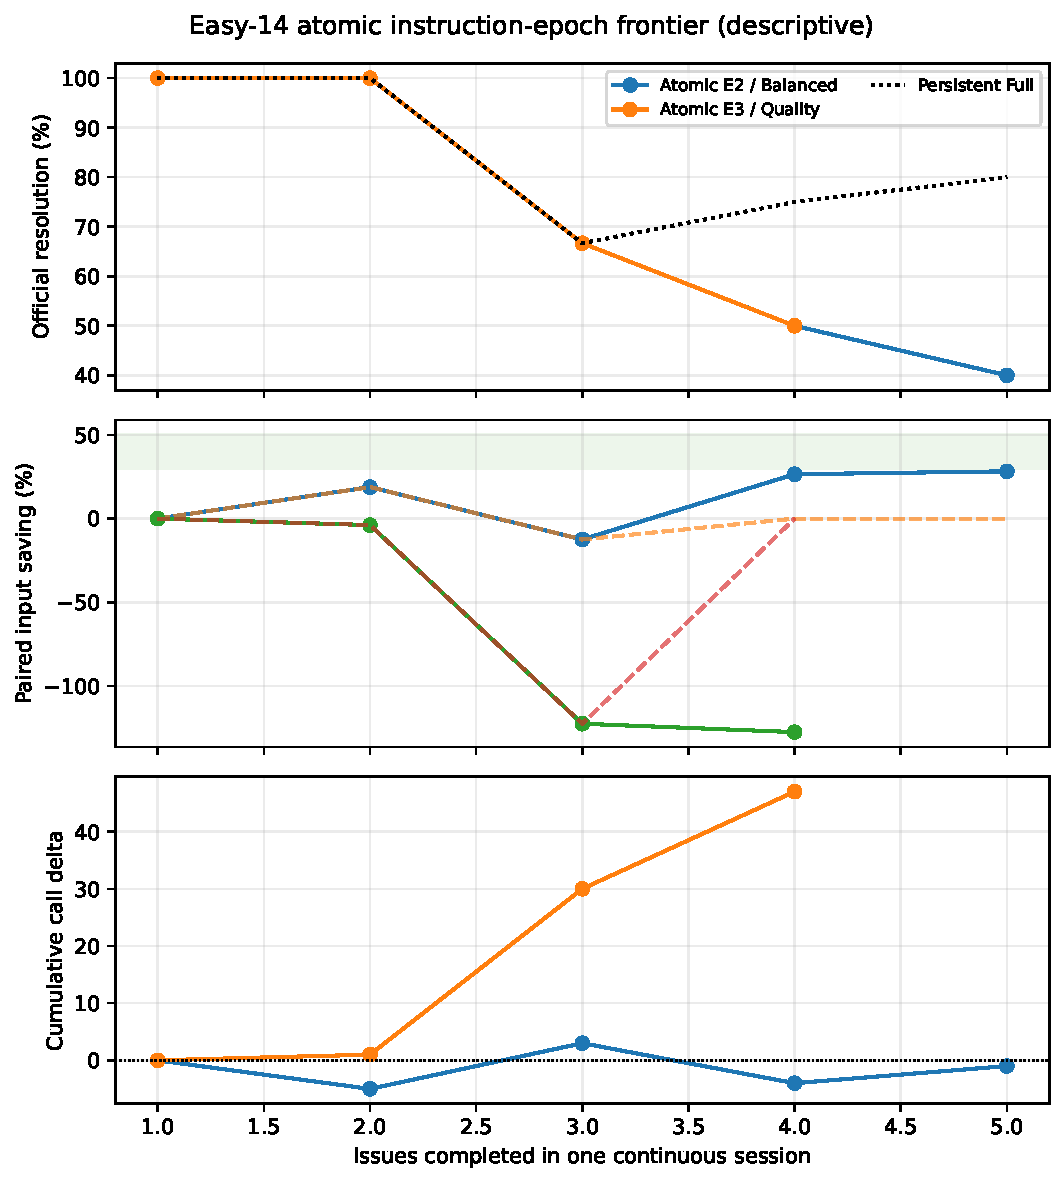
\includegraphics[width=0.86\linewidth]{../shared/results/paper8_5_agent_memory/easy14_atomic_profiles_ctx131k_v2/easy14_atomic_prefix_frontier.pdf}
\caption{Descriptive prefix curves for the stopped E2 and E3 arms.  Dashed
saving becomes zero after a lost paired \textsc{Full} success.  Prefix points
share tasks and are not independent confidence-interval samples.}
\label{fig:easy14-atomic-prefix-frontier}
\end{figure}

\section{Detailed Adaptive Policy Campaign}

Every reported strategy has a stable identifier, a predeclared rationale,
configuration coordinates, primary matched comparison, predicted failure mode,
and implementation status in
\path{multi_issue_strategy_registry_v1.json}.  We do not execute a blind
Cartesian product.  Simple families are first isolated at two and three issues;
a configuration that is low-saving, quality-losing, or call-inflating is
stopped.  A mixture is admissible only when each parent has an interpretable
effect and at least one parent is nondominated.  The combination then changes
one coordinate at a time and is compared with each parent plus a matched-token
tail.  Only nondominated configurations advance to four and five issues and to
held-out sequences.  This preserves an argument for every tested cell without
turning exploratory search into confirmatory evidence.

\begin{table}[H]
\centering
\small
\caption{Adaptive campaign stages. Frozen agreement prunes experiments but
never substitutes for autonomous quality.}
\begin{tabular}{>{\raggedright\arraybackslash}p{0.20\linewidth}
                >{\raggedright\arraybackslash}p{0.25\linewidth}
                >{\raggedright\arraybackslash}p{0.43\linewidth}}
\toprule
Stage & Arms & Advancement rule \\
\midrule
Mechanism & Every simple rule & Predicate, serialization, accounting, and
fail-closed tests must pass. \\
Frozen discovery & Simple rules and matched controls & Stop low-saving arms
with rapid action-proxy loss; retain mechanism controls without promoting them. \\
Bounded autonomous & Nondominated or information-preserving candidates & Run
one to three tasks with repeated \textsc{Full}; require official success before
task expansion. \\
Combination search & Only promoted parents & Hill-climb one parameter at a
time; do not combine stopped or dominated arms. \\
Confirmation & Frozen policy set on held-out tasks & Report task-level quality,
gross/net saving, calls, recovery, and uncertainty. \\
\bottomrule
\end{tabular}
\end{table}

\subsection{From a frontier to confirmation candidates}

The curve is the product interface, not merely a paper visualization.  A
developer needs official resolution, calls-to-solution, divergence, and
rediscovery; an operator needs fallback frequency, realized retention, and an
auditable per-session policy decision; an infrastructure buyer needs
failure-aware saving, cost per resolved issue, concurrency capacity, and a
quality confidence interval.  We therefore predeclare four logical destinations
without assigning a winning policy in advance: \textsc{Agent-Full} is the
no-selection correctness control; \textsc{Agent-Quality},
\textsc{Agent-Balanced}, and \textsc{Agent-Economy} choose the highest-saving
nondominated frozen point subject to lower sequence-clustered quality-delta
bounds of $-2$, $-5$, and $-10$ percentage points, respectively.  The latter
also requires at least 20\% failure-aware saving.  Balanced and Economy must
improve cost per resolved issue; Quality and Balanced must not materially
inflate calls among joint successes.

These names remain candidates until held-out autonomous confirmation. Frozen
next-action agreement alone cannot promote a profile, and insufficient data
cannot be converted into confidence by pooling requests, repeated executions,
or different sequence strata. The complete logical-to-runtime contract is
versioned in \path{paper4_5_profile_promotion_contract_v1.json}. Paper~4.5 may
claim a runtime-qualified profile only after realizing the identical frozen
logical plan while independently passing 100\% parity, sparse-K/V identity, and
lifecycle gates.

The adaptive rule is versioned before each discovery stage. Current whole-group
H1/H2a combinations are stopped because they lose the action proxy rapidly for
small savings; H4 remains an aggressive mechanism bound. Matched token tail
and positional materializers remain controls rather than parents. Structured
evidence receives a bounded autonomous probe because it preserves all causal
groups, but it does not expand unless task quality passes. This pilot-informed
pruning is exploratory. Final profile claims use a subsequently frozen policy
set and held-out tasks, preventing adaptive search from being mistaken for
confirmatory evidence.

\subsection{Pilot structural screen}

Before issuing counterfactual model calls, we ran the recordizer and selector
over three successful mini-swe-agent reference trajectories containing 69
historical model decisions. The full grid contains five budget fractions, four
head floors, five tail floors, five initial middle policies, and two DAG-first
compositions, for 48,300 selection decisions and 2,100 aggregated cells. This
screen uses a whitespace
counter and is therefore evidence only about structural feasibility, not model
token counts or policy quality.

Table~\ref{tab:structural-pilot} shows one illustrative slice with one first
turn and two latest turns retained. Whole causal bundles leave some budget
unused. Conversely, immutable and mandatory state can exceed the ceiling. At a
90\% request the basic head--tail policy overflows on 16 of 69 decisions, while
the role-aware progress spine overflows on 22 of 69. These are expected
round-up outcomes, concentrated when the trajectory is short; they demonstrate
why requested percentage, realized retention, and mandatory overflow must be
reported separately.

The legacy trajectories lack cwd, environment, output-completeness, and
resource-version fingerprints. The certificate-backed DAG arm therefore
correctly abstains and retains 100\% at $B=100\%$. Static Bash analysis exposes
458 superseded-current-state and 75 write-invalidated-state candidate
occurrences across the 69 growing prefixes, but no trace-exact duplicate and no
certified exclusion. These are repeated candidate occurrences, not unique
records, and are not removed. This is an instrumentation requirement, not a
negative quality result.

\begin{table}[H]
\centering
\small
\caption{Aggregate realized retention in the structural-only pilot for
$h=1,\tau=2$. These values do not measure next-action or task quality.}
\label{tab:structural-pilot}
\begin{tabular}{lrrrr}
\toprule
Policy & 90\% & 75\% & 50\% & 25\% \\
\midrule
Middle none & 55.5\% & 55.5\% & 55.5\% & 55.5\% \\
Progress spine & 66.5\% & 66.5\% & 66.5\% & 66.5\% \\
Middle recency & 85.9\% & 76.7\% & 59.6\% & 55.5\% \\
Middle lexical & 89.5\% & 77.1\% & 59.6\% & 55.5\% \\
Spine + lexical & 91.6\% & 80.0\% & 67.4\% & 66.5\% \\
\bottomrule
\end{tabular}
\end{table}

\subsection{Persistent-session structural opportunity}

We composed three already successful real trajectories into an ordered
multi-issue session and counted tokens with the frozen Qwen3-Coder tokenizer.
This is a structural opportunity screen only: no replay or autonomous quality
claim follows from it.  Table~\ref{tab:persistent-session-pilot} contrasts full
persistent history, a conservative completed-episode spine, and retirement of
all completed episodes.  The latter is intentionally an aggressive diagnostic.

\begin{table}[H]
\centering
\small
\caption{Tokenizer-exact structural opportunity as completed issues accumulate.
Savings are relative to persistent \textsc{Full}; task quality and K/V reuse
remain unmeasured.}
\label{tab:persistent-session-pilot}
\begin{tabular}{lrrrr}
\toprule
Policy / issues & Final selected/full & Final save & Cumulative selected/full & Cumulative save \\
\midrule
Completed spine / 2 & 14,681/21,989 & 33.23\% & 380,891/534,359 & 28.72\% \\
Completed spine / 3 & 15,381/33,431 & 53.99\% & 632,632/1,147,100 & 44.85\% \\
Active only / 2 & 12,237/21,989 & 44.35\% & 329,567/534,359 & 38.32\% \\
Active only / 3 & 11,206/33,431 & 66.48\% & 497,808/1,147,100 & 56.60\% \\
\bottomrule
\end{tabular}
\end{table}

The displayed active-only rows are retained as a historical structural upper
bound but are not eligible policy evidence: their legacy configuration allowed
completed task statements to be removed.  Every subsequent experiment pins
all user-authored instructions.  Tool observations remain selectable based on
typed provenance even when the harness transports them with the user role.

Three deliberately fresh \textsc{Full} sessions consume 496,540 cumulative
message-content tokens.  The active-only persistent arm consumes 497,808,
only 1,268 tokens (0.26\%) more, while preserving a single logical session
identity.  Thus it provides essentially no logical-token saving over deliberate
fresh resets; its value is only automatic session hygiene for a developer who
does not reset the conversation.  This supports the proposed workload axis but
not yet the stronger claim that persistence improves either agent quality or an
engine: native K/V reuse, original-position
sparse correctness, prefix-cache comparison, and agent-level resolution are
deferred to Paper~4.5 after Paper~8.5 quality gates pass.  Auditable schedules,
composed traces, and decision rows are released under
\texttt{multi\_issue\_session\_v1}.

The decisive experiment therefore uses two additional strata.  Related issues
share a repository and can benefit from prior localization or architectural
knowledge; dependent issues share a workspace and may consume artifacts or
decisions produced earlier.  On independent cross-repository issues,
\textsc{Fresh-Per-Issue} is expected to dominate logically and serves as a
negative control.  On related and dependent sequences, a selective persistent
policy can be credited over fresh reset only if reduced rediscovery or improved
quality pays for every retained prior-episode token.

A one-decision frozen smoke further demonstrates why structural opportunity is
not a policy frontier. At two issues, completed-spine and active-only retention
materialize 35.02\% and 13.29\% of persistent history, but neither reproduces
the contemporaneous \textsc{Full} command. At three issues, the same policies
materialize 28.45\% and 11.90\% and both reproduce that command. In both cases
the contemporaneous \textsc{Full} call itself differs from the command stored
in the historical successful trajectory. The opposite outcomes and unstable
historical control prohibit a policy ranking; the artifact is retained only as
a mechanism and instability audit. Repeated autonomous official resolution is
the next quality gate.

\subsection{Repeat-confirmed two-issue persistent-session point}

An infrastructure-clean autonomous persistent-session experiment now
provides a repeat-confirmed point beyond the structural screen.  The ordered
cross-repository sequence is \texttt{django-15277} followed by
\texttt{pytest-7982}, with a clean workspace for each issue but one persistent
conversation identity.  Both persistent \textsc{Full} repeats resolve both
issues.  The R4/M2/V2 completed-episode spine keeps the completed task
statement, four recent completed turns, two mutation turns, and two
verification turns.  Its first issue is the paired \textsc{Full} episode by
exact path and SHA-256 identity; selection begins only for the second issue.

\begin{table}[H]
\centering
\scriptsize
\caption{Infrastructure-clean autonomous N=2 repeat evidence. Candidate
gross saving uses the candidate's own realized trajectory. Paired
failure-aware saving charges selected tokens against the declared persistent
\textsc{Full} trajectory and therefore also reflects avoided or extra calls.}
\label{tab:persistent-autonomous-discovery}
\begin{tabular}{lrrrrrr}
\toprule
Arm & Resolved & Calls & Full tokens & Selected tokens & Gross save & Paired save \\
\midrule
Persistent \textsc{Full}, repeat 1 & 2/2 & 42 & 330,537 & 330,537 & 0.00\% & -- \\
Persistent \textsc{Full}, repeat 2 & 2/2 & 39 & 292,686 & 292,686 & 0.00\% & -- \\
R4/M2/V2, paired to repeat 1 & 2/2 & 35 & 253,582 & 209,878 & 17.23\% & 36.50\% \\
R4/M2/V2, paired to repeat 2 & 2/2 & 35 & 253,582 & 209,878 & 17.23\% & 28.29\% \\
\bottomrule
\end{tabular}
\end{table}

All admitted traces have contiguous request indices, zero upstream failures,
the frozen model and tokenizer revisions, and official SWE-bench grading.  On
the selected second issue, R4/M2/V2 diverges at the first action but resolves
in eight calls in both repeats, versus 15 and 12 calls for paired
\textsc{Full}.  Thus exact trajectory agreement is not the utility endpoint.
Across the two paired sequences, the ratio-of-sums message-input saving is
32.65\%, calls fall from 81 to 70, and no \textsc{Full} success is lost.  The
macro mean of the two paired savings is 32.40\%.  This passes the predeclared
30--50\% gate, but the uncertainty unit remains one ordered sequence family:
the repeats measure execution stability, not population accuracy.

The first N=3 expansion does not qualify.  Its persistent-\textsc{Full}
controls resolve only 2/3 issues in both repeats because
\texttt{sphinx-8721} fails, so this sequence cannot establish preservation of
three successes.  R4/M2/V2 likewise resolves 2/3, but its paired savings vary
from $-37.40$\% to $47.70$\% as calls vary from 67 to 40.  A single exploratory
R2/M2/V2 execution reaches 45.31\% paired saving and 42 calls, but also resolves
only 2/3.  These results expose trajectory-cost variance and motivate replacing
the third issue with a repeat-qualified \textsc{Full} success before further
profile promotion.  The compact confirmation ledger, task-aware pairing
identities, artifact hashes, reductions, and curves are released under
\texttt{autonomous\_persistent\_spine\_confirmation\_v1}; the earlier
\texttt{autonomous\_multi\_issue\_frontier\_v1} remains the discovery record.

\subsection{Replacement N=3 reliability and the R4 rejection}

We replaced the non-repeatable Sphinx issue with
\texttt{scikit-learn-13135} and separated task capability from submission
reliability.  One preserved \textsc{Full} repeat produced correct saved
workspace patches for Django, Pytest, and Scikit-learn, but emitted non-diff
terminal payloads.  Its primary score is therefore 0/3; counterfactual
official regrading of the saved workspace patches is 3/3 and is reported only
as auxiliary workspace capability.  We do not retry this observation away or
substitute the auxiliary score for unconditional resolution.

After correcting the grading path, three independent infrastructure-clean
persistent-\textsc{Full} repeats resolve all three issues: 9/9 issue
resolutions and 3/3 all-solved ordered sequences.  Each uses 53 calls, with
522,479, 550,355, and 553,263 cumulative logical input tokens.  The artifacts
are distinct by path, timestamp, and SHA-256 identity.  Health and transport
failures are retained in immutable retry directories but excluded from this
denominator.

\begin{table}[H]
\centering
\scriptsize
\caption{Replacement N=3 R4/M2/V2 gate.  R4 shares issue 1 by exact
artifact identity and starts selection at issue 2.  Paired raw saving charges
R4 selected tokens against its corresponding persistent-\textsc{Full}
control; failure-aware saving is zero for both failed pairs.}
\label{tab:persistent-n3-r4-gate}
\begin{tabular}{lrrrrrr}
\toprule
Arm & Resolved & Calls & Full tokens & Selected tokens & Gross save & Paired raw \\
\midrule
\textsc{Full}, repeat 1 & 3/3 & 53 & 522,479 & 522,479 & 0.00\% & -- \\
R4/M2/V2, repeat 1 & 2/3 & 49 & 539,956 & 377,476 & 30.09\% & 27.75\% \\
\textsc{Full}, repeat 2 & 3/3 & 53 & 550,355 & 550,355 & 0.00\% & -- \\
R4/M2/V2, repeat 2 & 2/3 & 45 & 439,877 & 311,333 & 29.22\% & 43.43\% \\
\midrule
R4 aggregate & 4/6 & 94 & 979,833 & 688,809 & 29.70\% & 35.80\% \\
Paired \textsc{Full} aggregate & 6/6 & 106 & 1,072,834 & 1,072,834 & 0.00\% & -- \\
\bottomrule
\end{tabular}
\end{table}

R4 reaches the target 30--50\% interval only under the paired raw coordinate
and reduces calls from 106 to 94, but it loses the Scikit-learn success in both
repeats.  Unconditional R4 resolution and conditional preservation on paired
\textsc{Full} successes are therefore both 4/6.  The predeclared
failure-aware saving is 0\%, and the zero-loss quality gate rejects the arm
regardless of its apparent efficiency.  In one
failure, the agent identifies the correct \texttt{np.sort} edit, executes a
regex-based \texttt{sed} command that does not match, verifies the unchanged
line, and submits an empty diff.  In the other, it submits the right semantic
operation at invalid indentation.  These are task-level execution failures,
not grader failures.

The repetitions also expose an important control result.  The first three
R4 Pytest requests have identical selected-message hashes and token counts
across repeats, but different response hashes despite temperature zero.
Likewise, the first R4 Scikit request is byte-identical across repeats and
already produces different responses.  Temperature zero is therefore not a
bitwise replay guarantee for this backend.  Policy claims require repeated
official outcomes; exact logical-input identity is an audit control, not a
replacement for replication.  More conservative R6 and R8 arms are evaluated
only as adaptive repairs after this predeclared R4 rejection.  R6/M2/V2
restores 3/3 official resolution in its first execution, but Scikit-learn
expands to 27 calls and the ordered sequence to 63 calls versus 53 for paired
\textsc{Full}.  R6
materializes 538,318 of 807,886 tokens on its own inflated trajectory, a
33.37\% candidate-gross saving, yet paired \textsc{Full} consumes only 522,479
tokens.  Its paired raw and failure-aware saving are both $-3.03$\%, so it
fails the saving and no-call-increase gates.  This is precisely why a
retention-only curve is not a utility frontier: the policy can remove a large
fraction of each prompt while causing enough extra decisions to increase total
consumption.  An independent R6 execution reverses the apparent tradeoff: it
uses 46 calls and materializes 326,252 of 456,267 candidate tokens, for
28.50\% candidate-gross and 37.56\% paired-raw saving, but loses the paired
Scikit-learn success.  Its failure-aware saving is therefore zero.  Across
the two R6 executions, official resolution is 5/6 versus 6/6 for paired
\textsc{Full}, and calls total 109 versus 106.  R6 is not a reliable repair.

R8/M2/V2 completes 3/3 issues.  It uses 59 calls, materializes 454,066 of
644,542 candidate tokens (29.55\% candidate-gross saving), and saves 13.09\%
against its 522,479-token paired \textsc{Full}.  The extra six calls and the
sub-30\% paired saving reject it under both remaining gates.  Table~\ref{tab:persistent-n3-repairs}
keeps candidate-local compression separate from paired utility.

\begin{table}[H]
\centering
\scriptsize
\caption{Adaptive N=3 repairs.  Failure-aware saving is zero for an execution
that loses a paired \textsc{Full} success; each row remains visible.}
\label{tab:persistent-n3-repairs}
\begin{tabular}{lrrrrrr}
\toprule
Arm & Resolved & Calls & Selected & Gross save & Paired raw & Failure-aware \\
\midrule
R6/M2/V2, execution 1 & 3/3 & 63 & 538,318 & 33.37\% & $-3.03$\% & $-3.03$\% \\
R6/M2/V2, execution 2 & 2/3 & 46 & 326,252 & 28.50\% & 37.56\% & 0.00\% \\
R8/M2/V2, execution 1 & 3/3 & 59 & 454,066 & 29.55\% & 13.09\% & 13.09\% \\
R4/M2/V2/P1, execution 1 & 3/3 & 47 & 332,269 & 30.02\% & 36.41\% & 36.41\% \\
R4/M2/V2/P1, execution 2 & 3/3 & 44 & 299,078 & 28.23\% & 45.82\% & 45.82\% \\
\bottomrule
\end{tabular}
\end{table}

Figure~\ref{fig:persistent-n3-frontier} makes the gate explicit in the primary
failure-aware coordinate.  R4 is charged zero saving after losing paired
successes; the two R6 outcomes average $-1.52$\% failure-aware saving after
ordered-sequence-family clustering; R8 remains well below the target band.
P1 is the first arm to enter the target band while preserving every paired
success: its two executions average 41.11\% failure-aware saving and 7.5 fewer
calls.
These points are descriptive measurements of one ordered three-issue family,
not a population interval.  Repeated executions measure reliability and are
not counted as independent task identities.

\begin{figure}[H]
  \centering
  
\includegraphics[width=0.82\linewidth]{../shared/results/paper8_5_agent_memory/autonomous_persistent_spine_n3_combined_v1/curves/independent_cross_repository/quality_vs_persistent.png}
  \caption{Failure-aware quality--saving frontier for the replacement N=3
  cohort.  The shaded band is the predeclared 30--50\% target; P1 enters it
  while preserving all paired successes in both executions.  Error bars are absent
  because this cohort contains only one ordered sequence family.}
  \label{fig:persistent-n3-frontier}
\end{figure}

\subsection{Frozen Scikit first-divergence oracle}

The autonomous outcomes alone cannot separate selection from backend
trajectory variance.  We therefore freeze the R4 repeat-1 completed-episode
prefix and reconstruct the exact first Scikit-learn selected-message digest.
On this identical prefix, full materialization produces a valid Bash action in
5/5 requests, although two response and command hashes occur.  R4/M2/V2
produces the same format-invalid response in 5/5 requests.  Temperature-zero
backend variance is real, but it does not explain this stable arm difference.

The R4 prompt already contains every available prior verification and
finalization record and the two latest mutation turns per completed issue.  We
then restore each of its 25 retired causal groups separately.  The restorations
range from 82 to 2,513 tokens; 24/25 recover one valid action, and every valid
action is a semantically equivalent source-file search represented by three
exact command hashes.  Only a 139-token mutation turn remains invalid.  This
is strong evidence for a selection-induced prompt-conditioning failure, but
not for one missing Scikit-relevant fact: many unrelated old groups repair the
protocol.  Oracle trials remain diagnostic and do not enter policy-quality
curves.

The deployable counterfactual is consequently content-independent: retain one
clean completed action--observation exemplar per prior issue in addition to
the recent, mutation, verification, and finalization floors.  We denote this
R4/M2/V2/P1.  P1 selects the latest complete turn containing both a valid
assistant action and tool observation while excluding error, mutation,
verification, and finalization roles.  It uses no future action and is not the
oracle choice.  The digest-bound oracle and
guardrails are released under
\texttt{oracle\_scikit\_r4\_r01\_first\_request\_v1}.

Two independent autonomous P1 executions pass the predeclared discovery gate.
Both paired \textsc{Full} controls resolve 3/3 in 53 calls.  P1 resolves 3/3
in 47 and 44 calls, materializing 332,269 and 299,078 input tokens.  Relative
to contemporaneous \textsc{Full}, the savings are 36.41\% and 45.82\%, with
six and nine fewer calls.  The descriptive means are 41.11\% saving and 7.5
fewer calls.  Candidate-trajectory gross savings are 30.02\% and 28.23\%; the
difference from paired savings reflects avoided decisions rather than hidden
token accounting.  This result qualifies P1 for frozen transfer to the
Paper~4.5 native-K/V evaluation \emph{when equivalent episode metadata is
available}.  It does not yet establish generality across boundary-free
sessions, ordered sequences, agents, or model families.

\subsection{Boundary-free global retention}

The preceding policy is allowed to know which completed turns belong to each
issue.  We next remove that signal.  The model and selector receive one
continuous transcript with no episode identifier, completion marker, or
workspace-scope annotation.  The immutable floor contains the system prompt
and every user-authored instruction; mini-swe-agent tool observations remain
selectable even though its compatibility protocol transports them using the
user message role.  R4/M2/V2/P1 is then applied globally to assistant--tool
causal groups.  Thus this treatment measures retirement of interaction
history, not accidental deletion of a task statement.

\begin{table}[H]
\centering
\small
\caption{First autonomous boundary-free N=3 result.  ``Candidate gross''
uses the candidate's own unpruned trajectory counterfactual.  Paired saving
charges materialized candidate tokens against contemporaneous persistent
\textsc{Full}; failure-aware saving is zero after any lost paired success.}
\label{tab:persistent-global-boundary-free-r4}
\begin{tabular}{lrrrrrr}
\toprule
Policy & Resolved & Calls & Full tokens & Sent tokens & Gross & Paired / aware \\
\midrule
Persistent \textsc{Full} & 3/3 & 55 & 599,397 & 599,397 & 0.00\% & 0.00\% / 0.00\% \\
Global R4/M2/V2/P1 & 2/3 & 66 & 748,306 & 293,091 & 60.83\% & 51.10\% / 0.00\% \\
\bottomrule
\end{tabular}
\end{table}

The aggregate compression is therefore not a viable saving.  Django falls
from a 27-call success to an unresolved 40-call cap; Pytest improves from 14
to 9 calls and remains resolved; Scikit-learn remains resolved but rises from
14 to 17 calls.  Django's first action divergence occurs at request six, the
first request after a causal group is retired, while still in the first issue.
No prior-issue boundary exists at that point.  This localizes the failure to
an overly short global tool-history floor rather than missing task-boundary
metadata or a removed user prompt.  The predeclared adaptive response is to
retain more interaction history (global R8) and rerun the complete paired
cohort; R4 is rejected regardless of its 51.10\% raw paired saving.

This failure exposes a conflation in a flat global floor.  It uses the same
parameter both to protect the active issue and to retire completed work.  We
therefore introduce a two-level \emph{instruction-epoch} policy.  A genuine
provenance-typed user instruction begins an observable epoch; a tool result
transported with the user role does not.  The policy keeps the system prompt,
every user instruction, and the entire current epoch.  Only assistant--tool
causal groups before the latest instruction are eligible for retirement.
There is no evaluator task ID, episode marker, completion flag, or workspace
label in the selector input.  For independent repositories, the E0 treatment
retires all such older interaction detail.  For related or dependent work,
that retirement is only an opportunity oracle until resource-version and
dependency edges certify disconnection; otherwise the deployable policy must
fail closed.

Before spending another autonomous cohort, we replayed the clean 3/3
persistent-\textsc{Full} trajectories through E0 with the exact locked Qwen
tokenizer.  Table~\ref{tab:instruction-epoch-oracle} counts every growing
request.  It is fixed-trajectory logical opportunity, not evidence that a
selected model run still solves the tasks.

\begin{table}[H]
\centering
\small
\caption{Instruction-epoch opportunity on the clean N=3 persistent-\textsc{Full}
sequence. ``Interaction saving'' excludes the immutable system/user
instruction floor from both numerator and denominator.}
\label{tab:instruction-epoch-oracle}
\begin{tabular}{rrrrrr}
\toprule
Issues & Requests & Full tokens & E0 tokens & Whole saving & Interaction saving \\
\midrule
1 & 27 & 153,654 & 153,654 & 0.00\% & 0.00\% \\
2 & 41 & 328,401 & 232,193 & 29.30\% & 42.72\% \\
3 & 55 & 599,397 & 356,091 & 40.59\% & 59.56\% \\
\bottomrule
\end{tabular}
\end{table}

At N=3, immutable instructions account for 31.85\% of cumulative content
tokens.  This distinction resolves the apparent ``ten tasks imply 90\%
saving'' argument.  If equal-size independent tasks retain only the active
assistant/tool epoch, the ideal saving \emph{within interaction history} is
$1-1/N$ for the \emph{final request}, reaching 90\% at N=10.  It is not the
cumulative-session saving: in the one-equal-request-per-epoch abstraction,
that quantity is $1-2/(N+1)$, or 81.8\% at N=10.  Real sessions weight each
epoch by its number and size of growing requests.  Whole-request saving is
smaller again because system and user instructions remain pinned, and their
share can grow with $N$.  We therefore report final-request opportunity,
cumulative own-trajectory saving, and paired end-to-end saving separately.
The active autonomous E0 run is the behavioral test: any first-issue
difference remains backend variance because E0 is an exact logical no-op until
the second genuine instruction.
The exact evidence is released under
\texttt{instruction\_epoch\_oracle\_n3\_clean\_full\_v1}.

\begin{figure}[H]
  \centering
  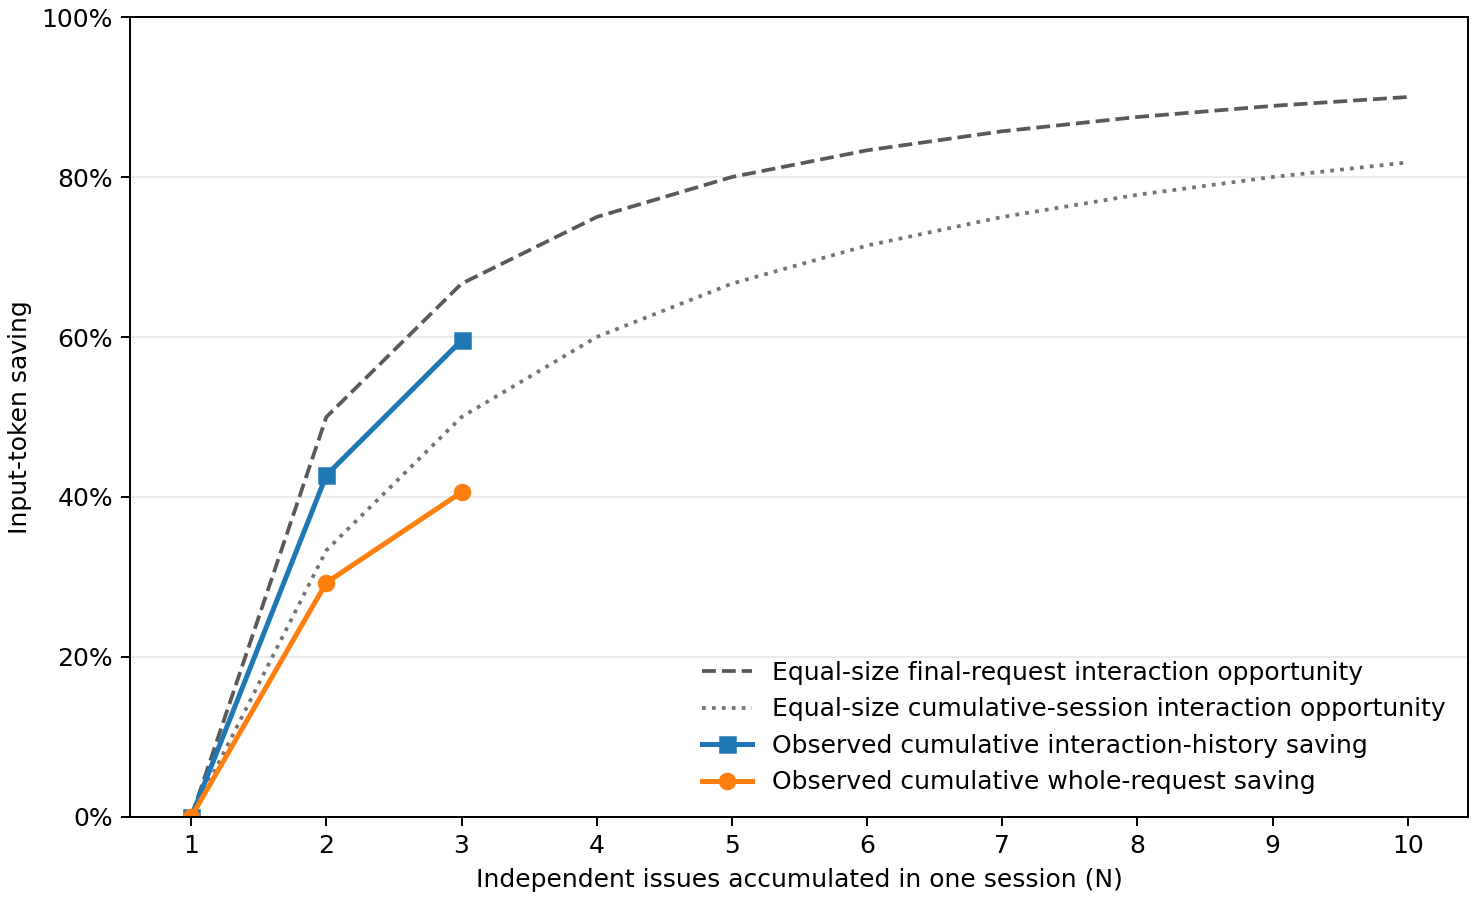
\includegraphics[width=0.88\linewidth]{../shared/results/paper8_5_agent_memory/instruction_epoch_oracle_n3_clean_full_v1/instruction_epoch_scaling.png}
  \caption{Empirical cumulative fixed-trajectory opportunity at N=1--3 and
  analytic equal-size interaction-history scaling to N=10.  The dashed curve
  is the final-request limit $1-1/N$; the dotted curve is the cumulative-session
  abstraction $1-2/(N+1)$.  Neither is a whole-request quality forecast.}
  \label{fig:instruction-epoch-scaling}
\end{figure}

The first autonomous E0 execution lands inside the desired saving region but
does not qualify because its contemporaneous control is not a clean accuracy
baseline.  Persistent \textsc{Full} resolves only Scikit-learn (1/3); Django
and Pytest end in grader/submission errors.  E0 preserves the Scikit-learn
success, resolves Pytest, and reproduces all 17 Django actions exactly because
the first issue is a logical no-op.  Table~\ref{tab:instruction-epoch-autonomous}
reports both denominators.

\begin{table}[H]
\centering
\small
\caption{First autonomous instruction-epoch E0 execution.  Paired saving uses
the contemporaneous persistent-\textsc{Full} denominator; candidate gross uses
E0's own unpruned trajectory.  Both rows are evidence-inadmissible for a quality
claim because the control contains grader errors.}
\label{tab:instruction-epoch-autonomous}
\begin{tabular}{lrrrrrr}
\toprule
Policy & Resolved & Calls & Full tokens & Sent tokens & Gross & Paired \\
\midrule
Persistent \textsc{Full} & 1/3 & 47 & 623,656 & 623,656 & 0.00\% & 0.00\% \\
Instruction epoch E0 & 2/3 & 44 & 567,826 & 320,375 & 43.58\% & 48.63\% \\
\bottomrule
\end{tabular}
\end{table}

Thus E0 loses zero contemporaneous \textsc{Full} successes, reduces calls by
three, and meets the 30--50\% paired-saving interval.  It nevertheless reaches
only 66.7\% unconditional resolution, below the predeclared 80\% gate, and the
sequence-level evidence is inadmissible.  We preserve rather than retry away
that baseline instability and run a fresh paired replication.  A positive
claim requires a repeat-qualified \textsc{Full} control, not merely conditional
preservation of one success.  The complete first execution is released under
\texttt{autonomous\_persistent\_instruction\_epoch\_n3\_e0\_v1}.

A fresh replication supplies the missing clean control and passes every
predeclared discovery gate.  Persistent \textsc{Full} resolves 3/3 in 66 calls.
E0 shares issue 1 exactly---a valid optimization because no earlier
instruction epoch exists---then independently executes issues 2 and 3.  It
resolves 3/3 in 64 calls, sends 506,776 tokens, and has an 839,601-token own-
trajectory counterfactual.  Its paired saving is 34.83\% and its own-trajectory
gross saving is 39.64\%.  Pytest falls from 14 to 10 calls; Scikit-learn rises
from 15 to 17, leaving two fewer calls in aggregate.

\begin{table}[H]
\centering
\small
\caption{Clean autonomous N=3 instruction-epoch replication.  Both rows are
admissible; E0 loses no official success and remains inside the frozen 30--50\%
paired-saving interval.}
\label{tab:instruction-epoch-clean-replication}
\begin{tabular}{lrrrrrr}
\toprule
Policy & Resolved & Calls & Full tokens & Sent tokens & Gross & Paired \\
\midrule
Persistent \textsc{Full} & 3/3 & 66 & 777,645 & 777,645 & 0.00\% & 0.00\% \\
Instruction epoch E0 & 3/3 & 64 & 839,601 & 506,776 & 39.64\% & 34.83\% \\
\bottomrule
\end{tabular}
\end{table}

This is the first valid boundary-free point in the requested quality--saving
region.  It qualifies E0 for repeat and sequence expansion, not for a universal
default: retirement assumes independent instruction epochs, the uncertainty
unit is one ordered sequence, and related/dependent work still requires a
resource-DAG disconnection certificate or fail-closed retention.  The evidence
is released under
\texttt{autonomous\_persistent\_instruction\_epoch\_n3\_e0\_replication\_v1}.

Before expanding to N=6, we screened six additional short Easy-14 identities
under ordinary \textsc{Full} and then repeated every first-pass success.  All six
resolve in the first screen, but only three resolve again: SymPy-16886,
Scikit-12585, and Django-16145.  Scikit-14496 and Django-14089 are genuine
second-run failures, while Django-15368 ends in an inadmissible
\texttt{patch\_apply\_failed} grader/submission error.  Calls also vary despite
temperature zero---for example, Scikit-12585 increases from 14 to 19 calls.
Thus ``baseline-success task'' is not a deterministic task label, and a policy
comparison must expose unconditional resolution and repeat reliability rather
than conditioning silently on one convenient \textsc{Full} trajectory.

\begin{table}[H]
\centering
\small
\caption{Current-endpoint N=1 qualification screen.  The second execution is
preserved even when it fails; only identities with two official successes
advance.}
\label{tab:instruction-epoch-n1-repeat-screen}
\begin{tabular}{lrrrrl}
\toprule
Identity & Calls A & A & Calls B & B & Advances? \\
\midrule
SymPy-16886 & 9 & pass & 10 & pass & yes \\
Scikit-12585 & 14 & pass & 19 & pass & yes \\
Scikit-14496 & 13 & pass & 22 & fail & no \\
Django-15368 & 16 & pass & 21 & error & no \\
Django-14089 & 22 & pass & 40 & fail & no \\
Django-16145 & 26 & pass & 26 & pass & yes \\
\bottomrule
\end{tabular}
\end{table}

The N=6 sequence combines those three new repeat-qualified identities with
Django-15277, Pytest-7982, and Scikit-13135, each of which already has multiple
admissible \textsc{Full} successes in the released persistent-session evidence.
The selector still receives no task ID, episode ID, completion flag, or
workspace scope: it observes only ordinary message roles and record
provenance.  Screen evidence is released separately under
\texttt{instruction\_epoch\_n1\_candidate\_screen\_v1} and
\texttt{instruction\_epoch\_n1\_candidate\_repeat\_v1}.

The autonomous N=6 execution exposes the distinction between local retention
and end-to-end efficiency.  E0 resolves all six issues, including one issue
that the contemporaneous \textsc{Full} control misses, and its own growing
trajectory sends 55.34\% fewer tokens than that same trajectory without
retirement.  However, E0 takes 114 calls versus \textsc{Full}'s 60.  Its
1,171,988 sent tokens exceed the control's entire 814,617-token workload, so
paired failure-aware saving is $-43.87$\%, not $+55.34$\%.  The run loses none
of the five \textsc{Full} successes, but it fails the no-call-increase and
30--50\% net-saving gates.

\begin{table}[H]
\centering
\small
\caption{Autonomous N=6 instruction-epoch result.  ``Gross'' uses each row's
own trajectory counterfactual; ``paired'' compares sent tokens with the
contemporaneous persistent-\textsc{Full} workload and therefore includes the
cost of extra calls.}
\label{tab:instruction-epoch-n6-e0}
\begin{tabular}{lrrrrrrr}
\toprule
Policy & Resolved & Calls & Full tokens & Sent tokens & Gross & Paired \\
\midrule
Persistent \textsc{Full} & 5/6 & 60 & 814,617 & 814,617 & 0.00\% & 0.00\% \\
Instruction epoch E0 & 6/6 & 114 & 2,624,244 & 1,171,988 & 55.34\% & $-43.87$\% \\
\bottomrule
\end{tabular}
\end{table}

This is a useful negative result rather than a failed mechanism: retirement
fires exactly as specified and preserves official resolution, but the model
uses the shorter context less efficiently.  We therefore predeclare E1 and E2,
which keep the immediately preceding one or two genuine-user instruction
epochs whole.  These policies consume no task identifier; they use only the
ordinary user-instruction boundaries already present in the transcript.  The
N=6 E0 evidence is released under
\texttt{autonomous\_persistent\_instruction\_epoch\_n6\_e0\_v1}.

The completed E1/E2 ladder rejects both repairs
(Table~\ref{tab:instruction-epoch-n6-ladder}).  Its contemporaneous
\textsc{Full} control resolves 4/6 in 62 calls, but the Django-15277 submission
ends in \texttt{patch\_apply\_failed}; the whole paired sequence is therefore a
preserved reliability observation, not admissible positive evidence.  E1
resolves 5/6 and loses no observed \textsc{Full} success, but its 70 calls
produce only 14.21\% raw paired saving and add 22 calls over the four jointly
successful issues.  E2 uses 60 calls and sends 21.93\% fewer tokens than the
control, but swaps outcomes: it gains Django-15277 and loses the control's
Django-16145 success.  The predeclared failure-aware charge is consequently
zero.

\begin{table}[H]
\centering
\scriptsize
\caption{N=6 instruction-epoch ladder. ``Gross'' compares each policy with
its own unpruned trajectory; ``raw paired'' uses the contemporaneous
persistent-\textsc{Full} token denominator; ``aware'' charges any lost control
success as zero saving.  No treatment qualifies.}
\label{tab:instruction-epoch-n6-ladder}
\begin{tabular}{lrrrrrrr}
\toprule
Policy & Resolved & Calls & Sent tokens & Gross & Raw paired & Aware & Lost \\
\midrule
Persistent \textsc{Full} & 4/6 & 62 & 830,776 & 0.00\% & 0.00\% & 0.00\% & 0 \\
E1: keep one prior epoch & 5/6 & 70 & 712,763 & 27.90\% & 14.21\% & 14.21\% & 0 \\
E2: keep two prior epochs & 4/6 & 60 & 648,571 & 16.48\% & 21.93\% & 0.00\% & 1 \\
\bottomrule
\end{tabular}
\end{table}

The ladder also identifies backend variance directly.  E1 and E2 remove
nothing on issue 2: the first request is byte-identical to \textsc{Full}, all
three runs use temperature zero, top-$p$ one, seed zero, and 100\% realized
retention, yet \textsc{Full}'s first command differs.  E1 and E2 match for six
actions, diverge at action seven, and reconverge at action eight; both solve.
Thus action divergence before any exclusion cannot be attributed to memory
selection.  The released reducer reports identical-input divergence and
selection-active divergence separately and marks the ladder points
inadmissible in the curves.

A targeted issue-5 diagnosis freezes E2's successful four-issue prefix, resets
the Django workspace for every fork, and first repeats only the next request.
E2 retains 11,918 of 15,861 content tokens (24.86\% first-request saving) and
emits the same command in 5/5 repeats.  \textsc{Full} emits two commands in
five byte-identical repeats.  Restoring retired epoch 1 retains 13,945 tokens
and reproduces one \textsc{Full} command exactly; restoring epoch 2 retains
13,834 and produces a third command.  All four commands are semantically
equivalent searches for Django's \texttt{runserver} implementation.  The
first action therefore does not implicate either retired epoch.

We then repeat the complete autonomous task from that same prefix and base
workspace.  Two E2 forks both resolve officially in 13 calls with the
identical patch.  Each sends 188,720 tokens versus its 239,979-token
own-trajectory \textsc{Full} counterfactual (21.36\% gross saving).  Two
\textsc{Full} forks both fail official grading, in 8 and 18 calls, with
different incorrect patches.  Mean calls are equal at 13 and E2 sends 21.92\%
fewer tokens than the mean \textsc{Full} execution (188,720 versus 241,687).
This reversal does not show that pruning improves accuracy: it shows that the
ladder's single E2 loss is not a reproducible deterministic selection failure.
E2 remains below the 30\% target, and reliable promotion now requires
randomized, interleaved repeats over complete ordered sequences.  The complete
ladder and diagnostic are released under
\texttt{autonomous\_persistent\_instruction\_epoch\_n6\_ladder\_v1}.

Before spending another autonomous sequence, we screen hybrid floors on the
62 locked \textsc{Full} requests (Figure~\ref{fig:instruction-epoch-profile-screen}).
All user instructions and the active epoch remain whole.  E0 offers 48.22\%
fixed-trajectory gross saving at N=6; one clean protocol turn per older epoch
(P1) leaves 44.87\%; one mutation, verification, and protocol turn per older
epoch (M1/V1/P1) leaves 39.81\%.  Adding one or two ordinary recent turns per
older epoch yields 37.43\% and 35.61\%, respectively.  Keeping the most recent
old epoch whole (E1) yields 31.80\%.  Thus the desired 30--50\% opportunity
band is not the remaining problem.  The next autonomous candidate is
E0+M1/V1/P1, with R1/M1/V1/P1 as its conservative fallback; whether either
avoids E0's extra-call cost is the next gate.  Targeted pilots on the frozen
issue-5 prefix reject both.  M1/V1/P1 fails official grading after 18 calls
while saving 34.97\% on its own trajectory; R1/M1/V1/P1 fails in 9 calls while
saving 37.23\%.  Both independently produce the same incorrect patch, mapping
address \texttt{0} to Django's default address instead of \texttt{0.0.0.0}.
Because E2 resolves 2/2 from the same prefix, one old mutation, verification,
and protocol turn per epoch does not preserve all useful conditioning carried
by two complete epochs.  Neither hybrid advances.

That conclusion was incomplete because it compared coarse floors before
checking whether the serialized policies preserved a resolved conversation
structure.  A record-level oracle-alignment audit exposes the defect.  Global
R4/M2/V2/P1 removes 37.2--79.1\% of the active issue's interaction tokens at
the N=3--5 prefixes.  E0 removes none of the active issue, but pins every old
user task statement while deleting every corresponding completion turn.  At
N=5 its request therefore begins with five consecutive task descriptions,
four of which appear unanswered.  E1 and E2 merely leave one or two such
epochs whole; they do not express the actual invariant.

We add F1: retain the latest terminal finalization action--observation bundle
from each retired instruction epoch.  E0+F1 consumes no evaluator task ID,
episode label, or workspace boundary; it uses the same genuine-user
instruction epochs and typed finalization records already present in the
ordinary history.  Evaluator episode identity is used only afterward to score
alignment against an independent-cross-workspace oracle that retires prior
interaction detail but keeps one closure bundle per pinned prompt.

\begin{table}[H]
\centering
\small
\caption{Tokenizer-exact structural alignment on locked persistent-\textsc{Full}
prefixes.  E0+F1 keeps the active issue whole and exactly matches the initial
closure oracle, which later autonomous tests falsify as behaviorally
insufficient.  Structural alignment is not autonomous quality evidence.}
\label{tab:closure-oracle-alignment}
\begin{tabular}{rrrrr}
\toprule
Completed issues & E0+F1 saving & Active removed & Oracle P/R & Orphaned prompts \\
\midrule
2 & 13.8\% & 0.0\% & 100\% / 100\% & 0 \\
3 & 52.7\% & 0.0\% & 100\% / 100\% & 0 \\
4 & 52.6\% & 0.0\% & 100\% / 100\% & 0 \\
5 & 43.7\% & 0.0\% & 100\% / 100\% & 0 \\
\bottomrule
\end{tabular}
\end{table}

The corresponding frozen issue-5 ablation isolates closure from backend
variance.  The initial four arms share one canonical 15,861-token request and
are interleaved for three repeats.
\textsc{Full} produces one valid, repeat-identical search in 3/3 trials.  E0
selects 7,621 tokens (51.95\% saving) but produces no valid one-command action
in 0/3: its response enumerates all five issue statements as simultaneous
unrelated problems and emits four command blocks.  E0+F1 selects 8,627 tokens
(45.61\% saving) and restores one valid, repeat-identical current-Django search
in 3/3.  E2 is also valid in 3/3 but selects 11,918 tokens (24.86\% saving).
This directly implicates orphaned prompt closure rather than loss of active-
issue evidence, but the autonomous E0+F1 fork then fails after only three
actions: retaining the historical finalization also exposes the old submission
sentinel as an action exemplar.  Two synthetic replacements fail in opposite
ways.  A Bash \texttt{true} closure is copied in 3/3 frozen trials; a text-only
assistant/user closure identifies the active issue but emits no command in
3/3.  Closure semantics and action-protocol exemplars therefore cannot be
conflated.

The next treatment retires a prior instruction epoch atomically, including its
old user prompt, but only when the epoch itself contains complete terminal
evidence and a newer genuine user instruction exists.  It consumes no task ID,
evaluator episode boundary, repository name, or workspace-reset signal.  If
terminal evidence is absent, the old prompt remains.  Active-only atomic
retirement selects 1,507 tokens (90.50\% frozen-prefix saving) and produces a
valid stable search in 3/3, yet its autonomous fork fails after 22 calls with
an incorrect address-parsing patch.  The selected request at every decision
still contains the complete active epoch; the failure is not within-task
truncation.

This result, combined with E2's 2/2 same-prefix successes, motivates one causal
bracket rather than a grid: retain the two most recent natural successful
epochs as behavioral exemplars and atomically retire every older closed epoch.
The resulting atomic-E2 arm selects 8,707 tokens on the frozen request
(45.10\% saving) and yields one identical valid current-task search in 3/3.
Two independent reset-workspace autonomous forks resolve officially in 16
calls each, each sending 185,387 of 299,851 cumulative message-content tokens
(38.17\% saving) and producing the same patch.  Atomic E2 uses three more calls
than the two E2 diagnostic successes and four more than the older independent-
session reference, so it is a repeat-qualified single-task quality-preserving
point, not yet a no-call-increase default.

\begin{table}[H]
\centering
\small
\caption{Same-prefix autonomous diagnosis on Django-16145.  Savings use each
run's own full-history counterfactual; rows are not a population accuracy
estimate.}
\label{tab:atomic-epoch-bracket}
\begin{tabular}{lrrr}
\toprule
Policy & Official solves & Calls & Cumulative saving \\
\midrule
Persistent \textsc{Full} & 0/2 & 8, 18 & 0.00\% \\
E2, old prompts pinned & 2/2 & 13, 13 & 21.36\% \\
Atomic active-only & 0/1 & 22 & 71.03\% \\
Atomic E2 & 2/2 & 16, 16 & 38.17\% \\
\bottomrule
\end{tabular}
\end{table}

Artifacts, including the negative closure controls, are released under
\path{policy_oracle_alignment_n2_n5_v1}.  Atomic E2 now advances to a
held-out-task gate with the policy frozen; no broader parameter sweep is
justified by one task identity.

\begin{figure}[H]
\centering
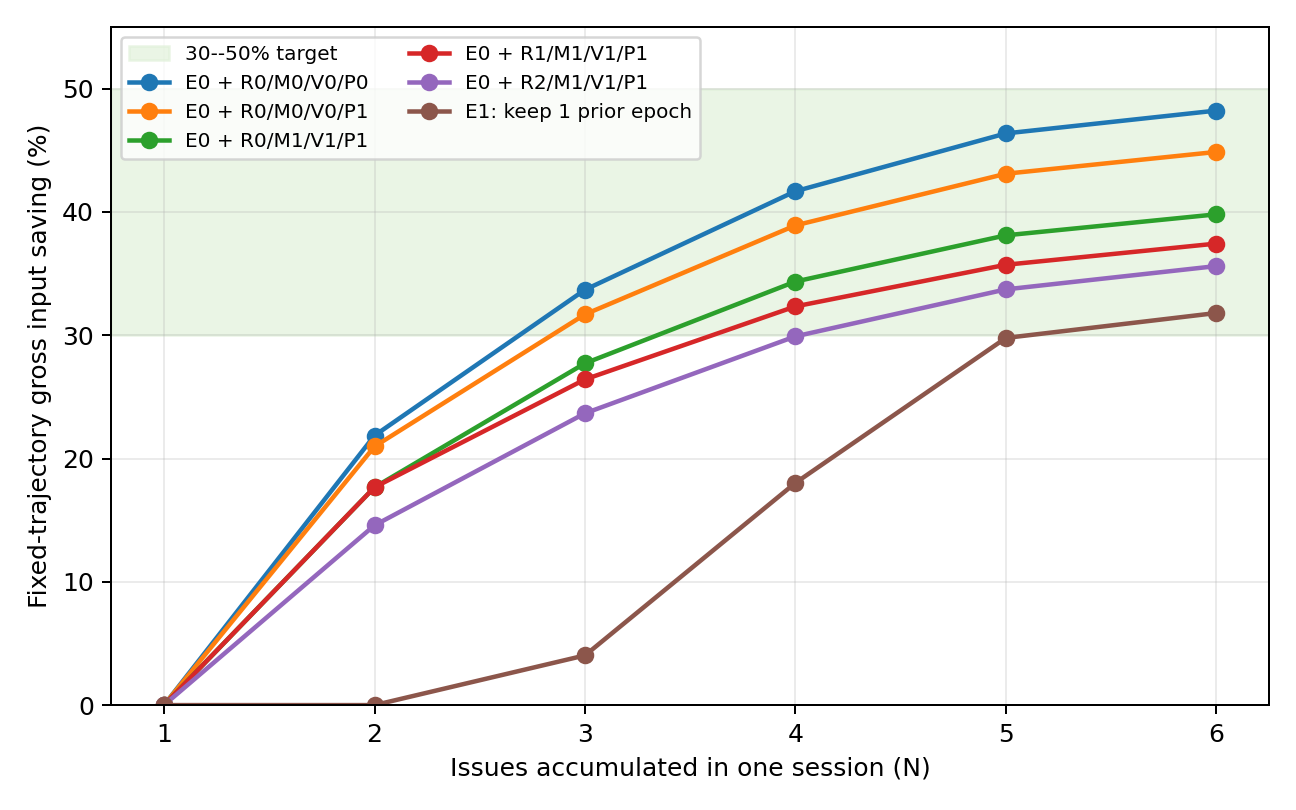
\includegraphics[width=0.94\linewidth]{../shared/results/paper8_5_agent_memory/autonomous_persistent_instruction_epoch_n6_ladder_v1/diagnostics/profile_screen/profile_saving_by_n.png}
\caption{Fixed-trajectory logical opportunity as independent issues accumulate
in one boundary-free session.  The shaded region is the 30--50\% target.  The
curves freeze model actions and therefore do not measure accuracy or
calls-to-solution.}
\label{fig:instruction-epoch-profile-screen}
\end{figure}

We also ran a structural-only opportunity screen for H1--H4 over the 23
growing prefixes of the first instrumented trajectory, with $h=0$, two tail
turns pinned, and a whitespace counter. After making explicit truncation
receipts fail closed, H1 with $K_f=0$ retires 938 cumulative whitespace tokens
(1.0\%); delaying to $K_f=4$ reduces this to 670 (0.7\%). Version-guarded H2a retires 308 (0.3\%), and H3 with $K_r=1$
retires 177 (0.2\%); $K_r\geq2$ finds no opportunity on this trace. Guarded
H2b correctly abstains because the captured verification lacks an explicit
resource dependency. H4 with $K_x=2$ has the largest opportunity, 3,180 tokens
(3.5\%), while $K_x\geq3$ abstains after dependency pins. H1+H3 removes 1,115
(1.2\%), and all guarded rules plus H4 at $K_x=4$ remove 1,423 (1.6\%). These
are cumulative prefix occurrences rather than unique records, and they measure
neither tokenizer-exact saving, next-action quality, nor task success. Their
purpose is to confirm that the arms fire differently before spending model
calls; the frozen gate and first autonomous pilot follow below.

Repeating the screen with the pinned Qwen3-Coder tokenizer changes the counts
but not the ordering. Across 199,109 cumulative full-history tokens, H1 at
$K_f=0$ removes 2,660 (1.34\%), H2a removes 833 (0.42\%), H3 at $K_r=1$
removes 603 (0.30\%), and guarded H2b abstains. Aggressive H4 at $K_x=2$
removes 11,370 (5.71\%), whereas $K_x\geq3$ abstains under the dependency
pins. These are still opportunity counts, not behavior results.

\subsection{Long-horizon, high-retention opportunity screen}

We next applied the expanded grid to two officially resolved ordinary-text
\textsc{Full} trajectories: \texttt{django-15277} (26 decisions) and
\texttt{django-15368} (30 decisions).  Together their growing prefixes contain
284,848 exact Qwen3-Coder tokens; the decision-20-and-later suffix contains
127,332.  Table~\ref{tab:long-horizon-opportunity} reports token-removal
opportunity, not model behavior or task quality.

\begin{table}[H]
\centering
\small
\caption{Exact-tokenizer saving on long successful \textsc{Full}
trajectories. ``Late'' integrates only decision 20 onward.}
\label{tab:long-horizon-opportunity}
\begin{tabular}{lrr}
\toprule
Treatment & Whole run & Late suffix \\
\midrule
H3, $K_r=1$ & 6.23\% & 8.04\% \\
H3, $K_r=2$ & 0.73\% & 1.63\% \\
H1, $K_f=8$ + H3, $K_r=2$ & 1.24\% & 2.78\% \\
H1, $K_f=12$ + H3, $K_r=2$ & 0.83\% & 1.86\% \\
\bottomrule
\end{tabular}
\end{table}

The effect is phase dependent: every displayed treatment saves a larger
fraction late than over the full trajectory.  The conservative
$K_f=8,K_r=2$ combination retains 98.76\% overall but 97.22\% in the late
suffix, providing a high-retention candidate that fires on both task
identities.  The mechanism differs by task: H1 supplies the removals on
\texttt{django-15277}, whereas H3 supplies them on
\texttt{django-15368}.  More history is not automatically better, however:
$K_r\geq4$ and $K_x\geq6$ abstain on both traces, while immediate H3 and small
working sets remove substantially more and remain higher-risk arms.

A blind fixed tail does not provide a stable retention contract.  From
decision 20 onward, keeping the first turn plus the last 20 complete turns
retains 95.77\% on \texttt{django-15277} but only 86.38\% on
\texttt{django-15368}; shorter fixed tails diverge further.  Therefore the
behavioral experiment will use an exact per-decision matched-token tail, not a
shared nominal $K$.  The long-horizon structural and high-retention JSON
artifacts in the shared results directory preserve all cells and suffix
aggregates.

\subsubsection{Frozen quality at matched high retention}

We screened the $K_f=8,K_r=2$ combination on the same two late suffixes using
direct MLX and its 4-bit Qwen3-Coder-30B weights.  This runtime is a logical
ordinary-text consumer here; no engine-performance result is inferred.  Two
independent \textsc{Full} runs reproduce all 18 late responses and commands
exactly.  We rejected the original Ollama endpoint for this comparison: its
first \textsc{Full} replay matched all 30 historical responses, but an
identical late repeat matched only 4/11 contents and 7/11 commands.

Table~\ref{tab:long-horizon-frozen} pairs the semantic arm with a blind token
tail using its per-decision materialized-token ceiling.  To obtain a close
match while preserving role order, only the boundary tool observation may be
trimmed; assistant actions remain whole.  The tail underfills by 20 cumulative
tokens on \texttt{django-15277} and 60 on \texttt{django-15368}---0.065\% of
the semantic arm's pooled materialized count.

\begin{table}[H]
\centering
\small
\caption{Late-suffix direct-MLX frozen replay.  Exact command is relative to a
contemporaneous, repeat-qualified \textsc{Full} response.}
\label{tab:long-horizon-frozen}
\begin{tabular}{lrrrrr}
\toprule
Task & Decisions & Semantic ret. & Semantic cmd. & Tail ret. & Tail cmd. \\
\midrule
django-15277 & 7 & 97.12\% & 4/7 & 97.08\% & 6/7 \\
django-15368 & 11 & 97.29\% & 7/11 & 97.21\% & 8/11 \\
\midrule
Pooled & 18 & 97.22\% & 11/18 & 97.16\% & 14/18 \\
\bottomrule
\end{tabular}
\end{table}

The hypothesis receives only partial support.  Late exclusion opportunity is
indeed larger, but the current whole-group semantics do not exploit it better
than age alone.  Pooled exact content is tied at 7/18, while the tail preserves
77.8\% of commands versus 61.1\% for H1+H3 despite removing 80 more cumulative
tokens.  On \texttt{django-15277}, delayed H1 retires two search maps and the
assistant reasoning attached to them; the semantic arm records three immediate
reacquisitions, one policy-excess reacquisition, and one invalid action.  On
\texttt{django-15368}, H3 retires one older same-file read and first changes a
command at decision 23, two decisions before the tail.

This identifies a more precise next treatment.  State authority and reasoning
provenance must be separated: retain the assistant action/progress record, but
replace a superseded tool observation with a typed resource/version/span stub.
For discovery, preserve a compact unresolved-resource map rather than deleting
the search bundle.  The observation-only variants must again be compared with
token tail at matched materialized counts before any autonomous rollout.

\subsection{First instrumented frozen cohort}

We then executed the ordered frozen gate on
\texttt{scikit-learn\_\_scikit-learn-13135}.  The reference is a successful
23-decision ordinary-text mini-swe-agent trajectory using
\texttt{qwen3-coder:30b}, its pinned tokenizer, temperature zero, and restored
decision-point workspaces.  This is next-action evidence, not yet an
autonomous policy success rate.  Table~\ref{tab:first-frozen-cohort} compares
each arm directly with a contemporaneous seeded \textsc{Full} replay.
Temperature zero alone was insufficient: an unseeded repeat diverged at
decision 3 despite identical history through decision 20, so the original
unseeded policy matrix is quarantined rather than interpreted as selection
evidence. With seed zero, independent \textsc{Full}-A and \textsc{Full}-B runs
match all 23 generated contents byte-for-byte. Exact-command and
conservative-action rates use the 22 decisions on which \textsc{Full} emitted
a command; \textsc{Full}'s decision 22 is itself format-invalid.

\begin{table}[H]
\centering
\scriptsize
\caption{First instrumented frozen cohort. Saving is cumulative over growing
decision prefixes. ``Final'' means equality of the frozen decision-23 action,
not autonomous SWE-bench resolution.}
\label{tab:first-frozen-cohort}
\begin{tabular}{lrrrrrrc}
\toprule
Treatment & Mean ret. & Saving & Exact text & Exact cmd. & Cons. action & First text div. & Final \\
\midrule
\textsc{Full} & 100.0\% & 0.0\% & 100.0\% & 100.0\% & 100.0\% & -- & yes \\
\textsc{Full} repeat & 100.0\% & 0.0\% & 100.0\% & 100.0\% & 100.0\% & -- & yes \\
\textsc{Dag-Exclude}@100 & 99.8\% & 0.3\% & 91.3\% & 95.5\% & 95.5\% & 21 & yes \\
Matched token tail & 99.8\% & 0.3\% & 91.3\% & 95.5\% & 95.5\% & 21 & yes \\
H1 consumed search, $K_f=0$ & 98.9\% & 1.3\% & 52.2\% & 59.1\% & 68.2\% & 10 & yes \\
H1 consumed search, $K_f=4$ & 99.2\% & 1.0\% & 65.2\% & 68.2\% & 72.7\% & 14 & yes \\
H2a current-state read & 99.7\% & 0.4\% & 73.9\% & 77.3\% & 77.3\% & 17 & yes \\
H2b verified write & 100.0\% & 0.0\% & 100.0\% & 100.0\% & 100.0\% & -- & yes \\
H3 same span, $K_r=1$ & 99.8\% & 0.3\% & 91.3\% & 95.5\% & 95.5\% & 21 & yes \\
H4 working set, $K_x=2$ & 95.1\% & 5.7\% & 43.5\% & 54.5\% & 59.1\% & 9 & yes \\
H1+H3 & 98.6\% & 1.6\% & 47.8\% & 54.5\% & 59.1\% & 10 & yes \\
H2a+H3 & 99.4\% & 0.7\% & 73.9\% & 77.3\% & 77.3\% & 17 & yes \\
All guarded, $K_x=4$ & 98.3\% & 2.1\% & 52.2\% & 59.1\% & 63.6\% & 10 & yes \\
\bottomrule
\end{tabular}
\end{table}

Two mechanism findings are currently admissible. First, the instrumented trace supports one
\textsc{Trace-Exact-Operation-Result} certificate: two complete reads execute
the same command and return the same bytes for the same cwd, environment, and
resource version despite different reasoning prose.  Removing the older turn
saves only 603 cumulative tokens.  It changes decisions 21--22, from writing a
temporary diff to displaying it and then another invalid response, but returns
to the exact final submission action at decision 23.  Operational proof and
behavioral identity are therefore empirically distinct even in the strongest
current DAG tier.

The new within-observation token-tail control materially matches the DAG arm:
198,500 versus 198,506 cumulative materialized tokens. Both first change the
action at decision 21, preserve 95.5\% conservative action agreement, and
return to the exact final action. This one trace therefore does not yet show a
quality advantage for certified exclusion over recency at equal materialized
context.

Second, immediate H1 is too aggressive. Once a discovery result is consumed by
a concrete read and followed by a non-read transition, it removes one
190-token causal turn from each later prefix. The first text change occurs at
decision 10, the first command-string change at decision 12, and the first
conservatively different shell action at decision 13. Across all prefixes it
saves 2,660 tokens (1.34\%) but preserves only 68.2\% conservative action
agreement, with six immediate reacquisitions and one policy-excess
reacquisition. A search listing can remain a durable navigation map after one
file is opened. Delaying retirement to $K_f=4$ moves first conservative action
divergence from decision 13 to 16 and raises action agreement only to 72.7\%,
while five immediate reacquisitions remain. Delay is therefore insufficient:
the next H1 refinement must protect unresolved discovery branches or retain a
compact resource-map tombstone.

We implemented the strict unresolved-branch variant separately. It requires a
complete successful read/diff for every concrete resource returned by the
search, followed by the transition and $K_f$ delay. It abstains at every prefix
for all $K_f\in\{0,1,2,4\}$ on this trace because several discovered example
and test-file branches were never consumed. This is the correct conservative
outcome, but supplies no saving; a compact model-visible resource-map stub is
the next discriminating treatment.

H2a also fails as a safe-exclusion claim. Retiring a 119-token successful-write
turn after a complete same-version read/diff saves 833 cumulative tokens
(0.42\%), but first changes the shell action at decision 17, preserves only
77.3\% conservative action agreement, and changes action validity at decision
20. The current bytes represent file state, but they do not necessarily carry
the mutation's intent or the agent's progress state. A model-visible mutation
tombstone and the stricter verified-write H2b arm must therefore be evaluated
separately. H2b correctly abstains on this trace because the verification
record lacks explicit dependency metadata; its 23 outputs exactly match
\textsc{Full}. This is fail-closed correctness, not evidence that H2b can save
context when a verification receipt is available.

On this trace H3 at $K_r=1$ retires exactly the same older read as the
trace-exact DAG certificate, so all selected histories and generated outcomes
coincide: 603 cumulative tokens saved and 95.5\% conservative action
agreement. This does not establish the safety of H3's weaker version/span
criterion; a task containing non-identical overlapping reads is required to
separate it from byte-identical duplicate elimination.

H4 at $K_x=2$ reaches the largest saving, 11,370 cumulative tokens (5.71\%),
but changes the action as soon as it first fires at decision 9 and preserves
only 59.1\% conservative action agreement. Its zero immediate-reacquisition
count is not exculpatory: frozen decisions do not compound, and the generated
action can change without explicitly rereading the hidden resource. H4 remains
an aggressive capacity baseline, not a safe rule.

The two-rule combinations show no positive interaction on this trace. H1+H3
saves 3,263 cumulative tokens (1.64\%) but falls to 59.1\% conservative action
agreement, below H1 alone. H2a+H3 saves 1,436 (0.72\%) and retains H2a's
77.3\% action agreement because H2a has already changed the late decisions on
which H3 fires. The predeclared three-rule H1+H3+H2b arm is input-equivalent to
H1+H3 here because H2b abstains; it is recorded as a deterministic equivalence,
not charged as another model cohort.

Finally, the all-guarded treatment at $K_x=4$ saves 4,096 cumulative tokens
(2.06\%) with 63.6\% conservative action agreement. H2b and H4 abstain at that
setting, so this is effectively H1+H2a+H3. Its slight recovery relative to
H1+H3 despite removing more context demonstrates non-monotone model
sensitivity, not a robust policy improvement.

\subsection{Synthetic mechanism controls and structured result evidence}

The preceding negative outcomes could arise from a policy weakness, a rule that
does not implement its declared predicate, or an experiment-driver error. We
therefore added three small mini-swe-agent-shaped diagnostic trajectories with
predeclared dependency structure: (i) a search whose every returned branch is
subsequently read before a non-read transition, (ii) a versioned write followed
by two identical current-version reads and a resource-linked passing test, and
(iii) a long test observation whose decisive assertion and source location lie
away from both output boundaries. These are mechanism controls, not substitute
software-engineering benchmarks.

All structural gates pass: strict H1 removes exactly the consumed discovery
bundle; H2a/H2b remove exactly the witnessed write; H3 removes only the older
same-version duplicate read; and every predeclared necessary fact remains in
the selected history. The exercise also exposed and corrected an independent
replay-driver bug: the maximum-decision limit was applied before the minimum
decision, so selecting one late probe could silently execute zero calls.

We then queried one predeclared decision from each task using Ollama 0.30.8,
Qwen3-14B, its matching tokenizer, temperature zero, seed zero, and a
1,024-token output ceiling. Contemporaneous \textsc{Full} repeats reproduce all
3/3 contents and commands exactly. Table~\ref{tab:synthetic-diagnostics}
reports candidate behavior against those repeats. H3 is exactly inert in the
constructed same-version duplicate case. Strict H1 and verified-write H2b
change the exact terminal command, but both changes are between harmless
\texttt{echo} completion acknowledgements after the requested fix has passed;
this is a concrete reason to report completion-state/action equivalence beside
exact command identity.

\begin{table}[H]
\centering
\small
\begin{tabular}{lrrl}
\toprule
Treatment & Retained & Exact command & Diagnostic action \\
\midrule
Strict H1 consumed search & 85.75\% & no & equivalent completion no-op \\
H2b verified write & 78.53\% & no & equivalent completion no-op \\
H3 duplicate current read & 84.18\% & yes & exact \textsc{Full} command \\
Fixed head/tail tool result & 60.78\% & no & wrong phase: diff before edit \\
Lexical matched-span result & 80.02\% & no & targeted edit, correct file \\
Structured-evidence result & 66.88\% & no & targeted edit, correct file \\
\bottomrule
\end{tabular}
\caption{Single-decision synthetic mechanism diagnostics. Retained is the
tokenizer-measured materialized fraction of the full request. These rows test
implementation and controlled sensitivity; they do not estimate autonomous
task success.}
\label{tab:synthetic-diagnostics}
\end{table}

The structured-evidence materializer is deliberately not another positional
head/tail rule. It scores failure and traceback lines, source locations, diff
headers and hunks, source symbols, command-resource identities, and current
task/query matches; it preserves the return-code/output envelope and local
context around selected anchors. If no positive structural evidence exists, it
fails closed to the complete observation. In the long-result diagnostic, the
tool observation contains 856 tokenizer tokens. Structured evidence removes
315 of 951 total request tokens (33.12\%), versus 190 (19.98\%) for lexical
matching. Both produce a targeted edit on the correct file rather than the
exact \textsc{Full} command. Fixed head/tail loses the middle failure evidence
and produces a premature diff action. The generated edits were not executed,
so this is evidence about action phase and target rather than task correctness.
It nevertheless supports carrying structured evidence forward as a candidate
materializer, while whole-group H1/H2 retirement should next be compared with
model-visible resource-map and mutation receipts.

\subsection{Real oversized-observation materialization}

We next froze the successful \texttt{scikit-learn-13135} trajectory and applied
the same 512-token materialization threshold without removing any logical
record.  The trace contains a 2,526-token, 292-line source dump and later 685-
and 737-token observations.  A third current \textsc{Full} repeat reproduces
all 23 contents and all 22 defined commands byte-for-byte. This qualifies that
control but, as the threshold-repeat audit below shows, does not establish
universal endpoint determinism.

Across all 23 decisions, structured evidence reduces 199,109 cumulative
materialized tokens to 188,072, a 5.54\% saving.  It preserves 10/22 exact
commands and 12/22 conservatively equivalent shell actions; its 22/23
format-valid decisions equal \textsc{Full}'s validity count.  Thus selective
result evidence is more conservative than deleting causal groups, but it is
not behavior preserving even though every logical record remains selected.

An adaptive 256-token threshold repeat falls in the same effective
materialization class as 512 on this trajectory: both retain exactly 188,072
tokens at the same 23 decisions. The only additional record entering the
structured path at 256 has 259 tokens, and all of its lines are retained, so
the byte-identity no-op rule restores the canonical observation. Nevertheless,
the 256 repeat preserves 14/22 conservative actions versus 12/22 at 512 (and
12/22 versus 10/22 exact commands). This is same-input endpoint variability,
not a threshold effect. We therefore stop the remaining within-class threshold
sweep and require future curves to use observation-size breakpoints plus an
explicit model-visible request digest. A nominal parameter grid is not a
quality--saving curve when multiple settings materialize identical requests.

Table~\ref{tab:real-materialization} holds decisions 3--10 fixed to compare the
three result materializers on identical prefixes.  Structured evidence gives
up most of the attainable compression but doubles exact/conservative action
agreement relative to matched-span and quadruples it relative to fixed
head/tail.  All candidate actions are format-valid.  Because these are frozen
next actions over a successful source trajectory, not executed rollouts, the
table establishes a compression--agreement gradient rather than autonomous
task utility.

\begin{table}[H]
\centering
\small
\begin{tabular}{lrrr}
\toprule
Materializer & Materialized saving & Exact command & Conservative action \\
\midrule
Structured evidence & 4,335/57,480 (7.54\%) & 4/8 & 4/8 \\
Lexical matched span & 16,248/57,480 (28.27\%) & 2/8 & 2/8 \\
Fixed head/tail & 17,406/57,480 (30.28\%) & 1/8 & 1/8 \\
\bottomrule
\end{tabular}
\caption{Frozen real-trajectory comparison on decisions 3--10.  Logical
record retention is 100\% in every arm; saving is solely within oversized tool
observations.}
\label{tab:real-materialization}
\end{table}

The trace audit also supplies an important negative control.  The two long
Django cohorts contain, respectively, zero oversized observations and one
565-token observation for which the structured selector keeps every line.  An
initial nominal no-op nevertheless changed 2/11 commands because the harness
reconstructed the complete observation with \texttt{splitlines()} and join,
dropping trailing-byte detail while reporting identical token counts.  That
artifact is quarantined.  Complete-line selection now returns the canonical
record bytes, and a byte-identity regression test prevents recurrence.  This
is the text-materialization analogue of the cache-identity rule: zero measured
token change is not evidence of an identical model input.

Figure~\ref{fig:frozen-frontiers} collects the repeat-qualified frozen
comparisons without pooling incomparable decision cohorts.  It is intentionally
labelled as a proxy frontier: only autonomous official-resolution experiments
populate the accuracy--saving curve.  The figure makes the present screening
decision visible---whole-group heuristics lose agreement rapidly, matched
recency is a strong control, and structured materialization is the only current
candidate admitted to a bounded task-utility probe.

\begin{figure}[H]
\centering
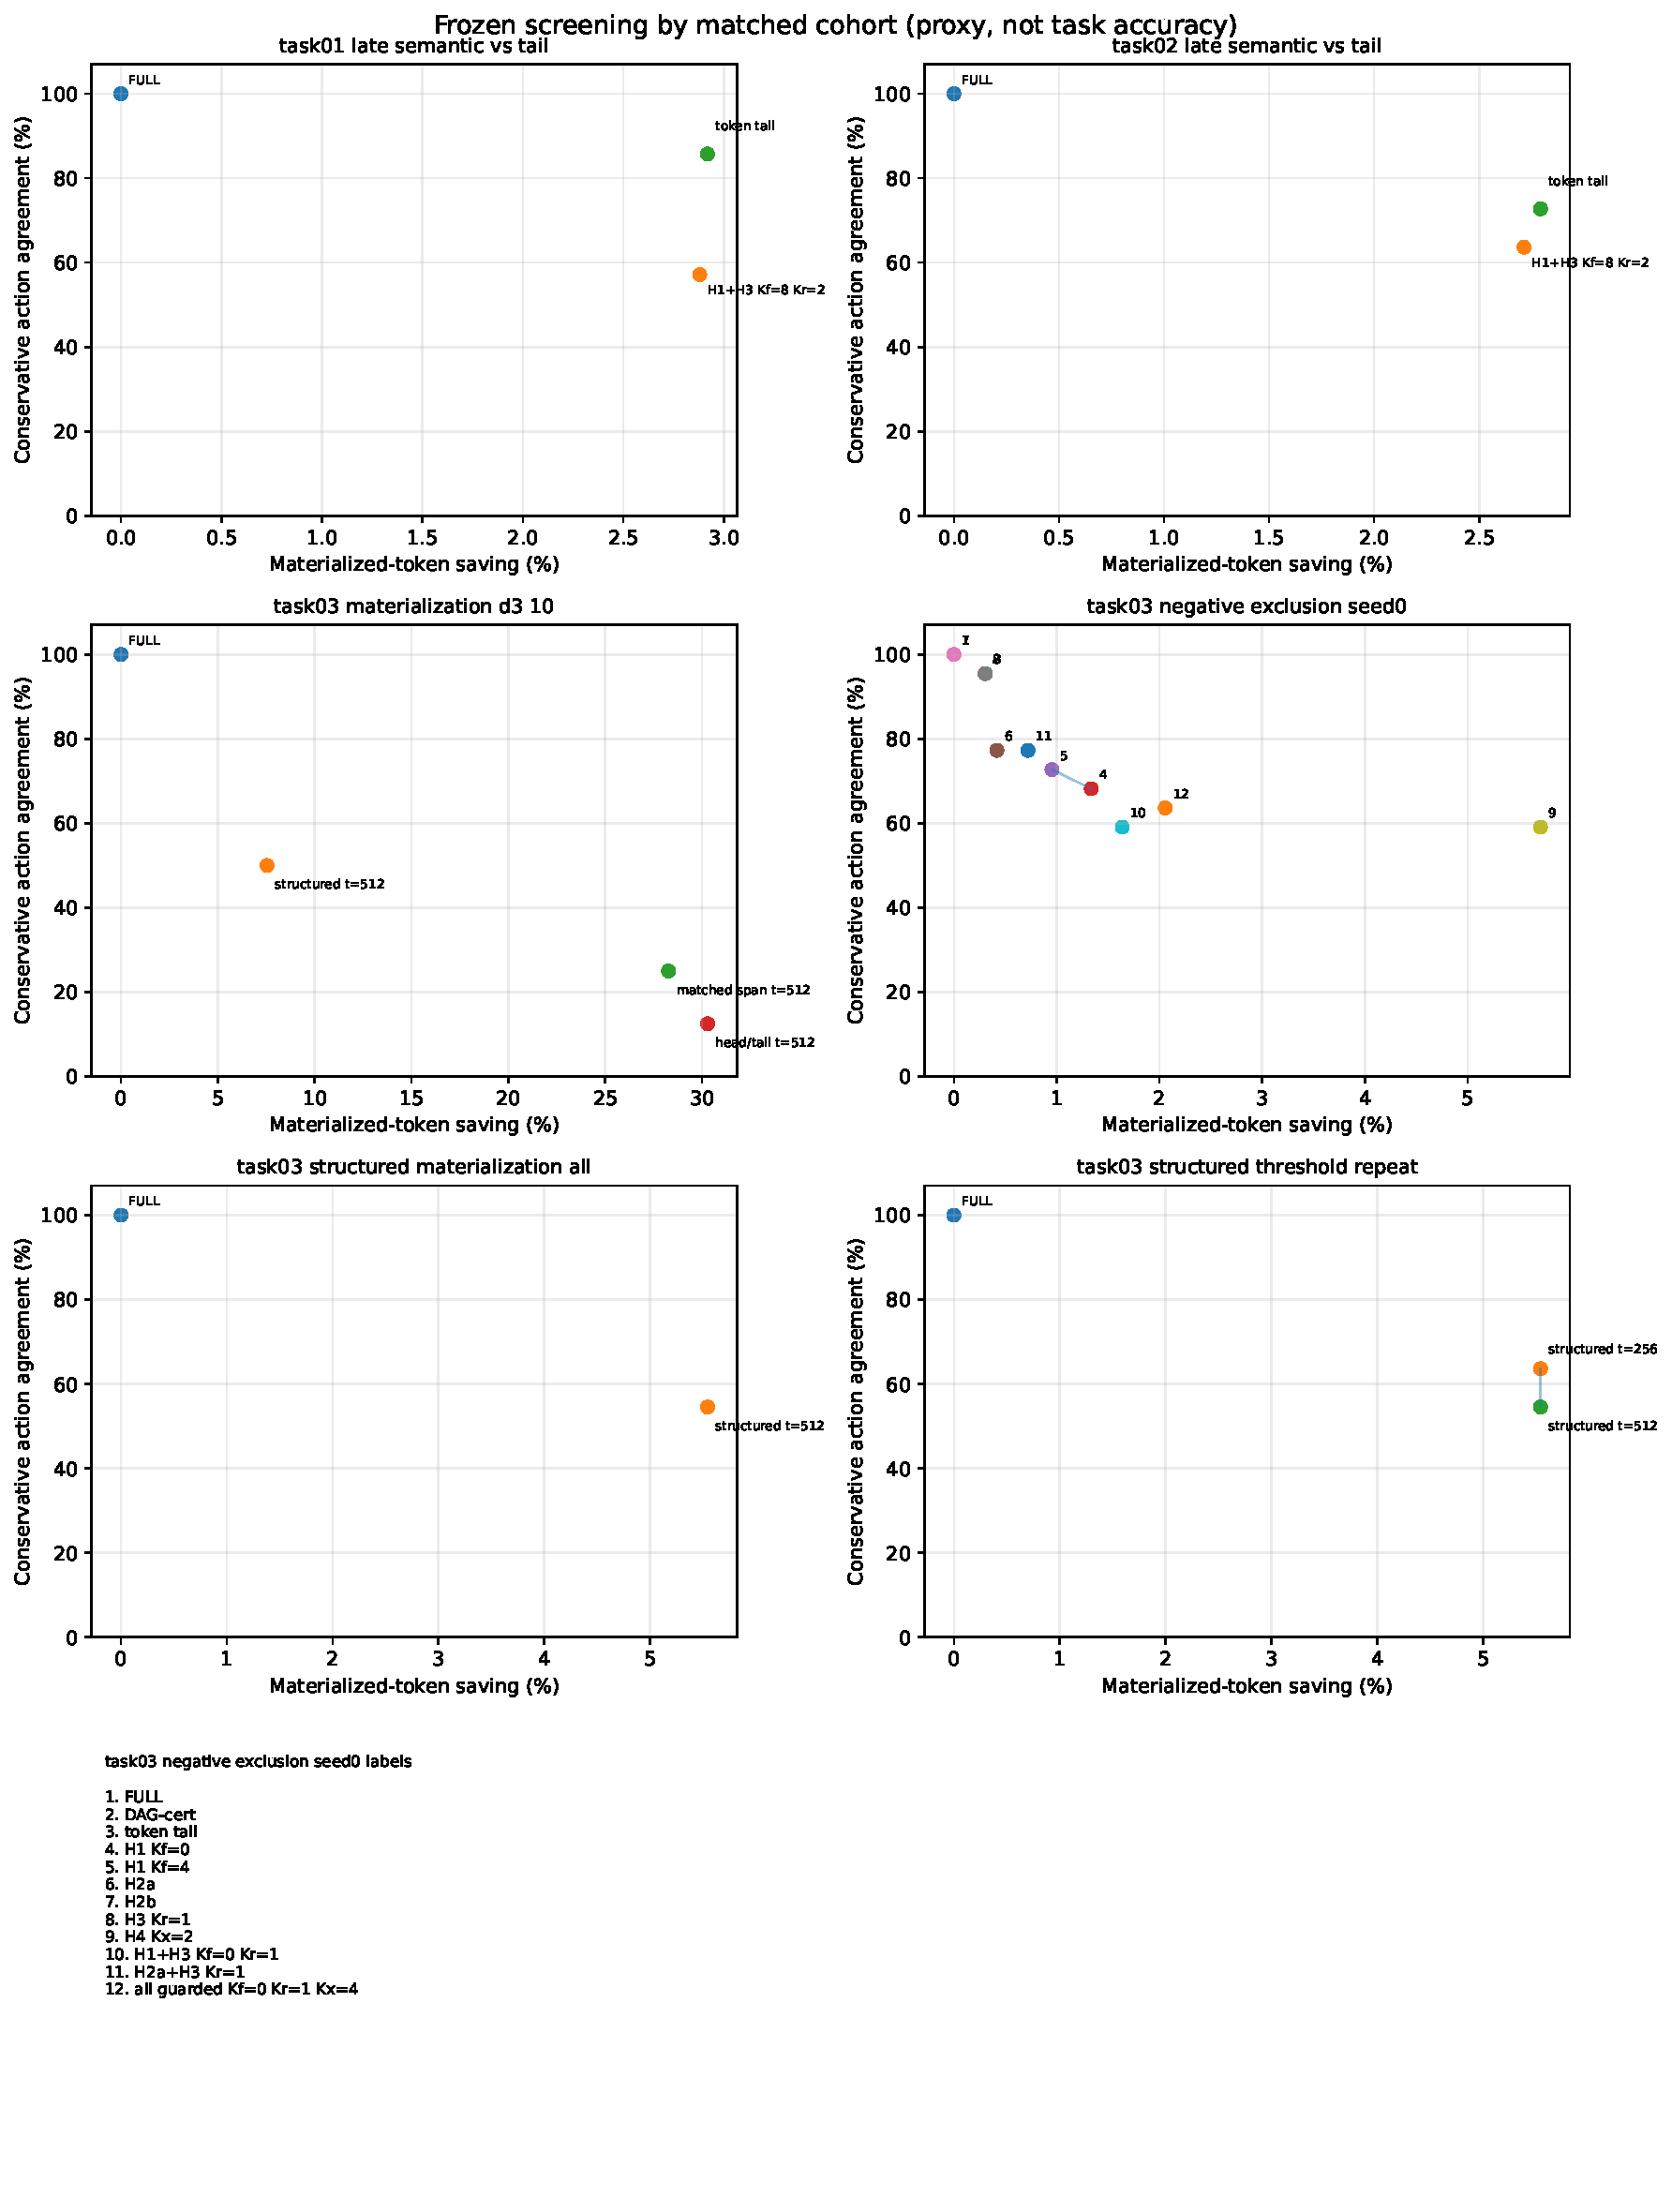
\includegraphics[width=0.88\linewidth]{../shared/results/paper8_5_agent_memory/tradeoff_curves/frozen_saving_vs_action_agreement.pdf}
\caption{Materialized-token saving versus conservative next-action agreement,
separated by matched frozen cohort. Agreement is diagnostic and is not task
accuracy.}
\label{fig:frozen-frontiers}
\end{figure}

\subsection{Autonomous structured-observation pilot}

We then ran the structured materializer autonomously on
\texttt{scikit-learn-13135}, still retaining every logical causal group.  The
512-token treatment resolves officially in 22 calls and materializes 159,482
of 169,850 trajectory-counterfactual message tokens, a 6.10\% gross saving. A
successful \textsc{Full} control resolves in 23 calls and consumes 197,796
tokens. A second \textsc{Full} execution stops after 19 calls with a nonempty
778-byte terminal workspace patch but submits an empty patch, so its primary
official outcome is failure. Thus the treatment is a promising one-task point,
not an accuracy estimate or a paired trajectory-saving claim: the two
\textsc{Full} trajectories have different lengths and outcomes. It advances
only to repeated same-host evaluation on multiple task identities. The compact
ledger is released under \path{autonomous_structured_task5_v1}.

\subsection{Model-visible resource and mutation receipts}

Binary H1/H2 deletion removes both payload and progress evidence.  We therefore
implemented a separate \emph{observation-receipt} realization: retain the
historical assistant action verbatim and replace only its paired tool
observation with a compact resource-map or mutation receipt derived from the
current prefix.  Receipt and source tokens are measured with the active model
tokenizer.  The treatment emits only when the receipt is strictly smaller;
otherwise it restores the complete canonical group.  Malformed pairs and
prefix-invalid witnesses fail closed under a distinct reason code.

This size gate was required empirically.  The first general JSON receipt
expanded the short synthetic H1 observation from 26 to 134 tokens and H2b from
15 to 133.  It increased total context and made the H1 response format-invalid.
After compacting the syntax and adding the gate, the candidate receipts are 43
and 46 tokens, respectively, so both short controls abstain.  Their serialized
requests are byte-identical to \textsc{Full}, and both contents and commands
reproduce exactly.  A receipt system must count its own disclosure cost; a
semantically sensible summary is not a saving when it exceeds its source.

To verify activation independently of this size boundary, we derived two
synthetic mechanism controls by appending 96 deterministic, semantically
irrelevant diagnostic lines only to the old H1 search observation or H2b
mutation observation.  Table~\ref{tab:receipt-activation} shows that the
receipt path then removes most payload while preserving the old action and a
model-visible state fact.  Every candidate emits a valid terminal completion
action, and role alternation, prefix-local witnesses, and absence of future
message leakage pass audit.  H1's identical-input \textsc{Full} repeats differ
in terminal wording, so its exact-command difference is not attributable.
H2b's \textsc{Full} repeats are exact, but its single receipt and deletion
outputs both differ only in terminal \texttt{echo} wording.  These rows qualify
the mechanism, not autonomous utility.

\begin{table}[H]
\centering
\small
\begin{tabular}{lrrr}
\toprule
Synthetic treatment & Full/materialized & Saving & Action phase \\
\midrule
H1 whole-group drop & 1,449/337 & 76.7\% & terminal completion \\
H1 observation receipt & 1,449/410 & 71.7\% & terminal completion \\
H2b whole-group drop & 1,410/278 & 80.3\% & terminal completion \\
H2b observation receipt & 1,410/385 & 72.7\% & terminal completion \\
\bottomrule
\end{tabular}
\caption{Size-gated receipt activation controls.  H1 replaces a 1,082-token
observation with 43 tokens; H2b replaces 1,071 with 46.  The receipt costs more
than deletion because it retains the original assistant action.}
\label{tab:receipt-activation}
\end{table}

The next receipt arm should remain separately labelled.  A
\emph{witness-attached receipt} would remove the old pair and append a compact
fact to the already selected downstream H1 read, H2a current-version read/diff,
or H2b verifier.  It can save small 44--49-token groups without introducing an
extra role pair, but it moves evidence later and discards the original
action/progress text.  It therefore requires its own frozen replay and
autonomous qualification rather than being folded into observation-receipt.

We then applied the portable v4 policy to decisions 22--24 of the successful
real Django task 15277 trajectory.  Two contemporaneous
\textsc{Full} controls agree on two of three exact next commands and first
differ only at decision 24.  Two semantic-receipt repeats produce
byte-identical model output at all three decisions, but agree with the first
\textsc{Full} control on only one of three commands and first differ at
decision 22.  The treatment materializes 20,893 of 21,907 content tokens, a
4.63\% saving, by replacing three older same-version reads at each decision.
This is a bounded action probe, not task-accuracy evidence.  It nevertheless
shows why selection evidence and presentation must be separated: the phrase
``older read superseded'' is model-visible text and can itself prime a
consolidation action even though the newer source evidence remains selected.

The default portable realization therefore keeps rule, resource, version,
completeness, and witness evidence entirely in out-of-band request metadata.
If the chat protocol requires a paired observation, it emits only a role-valid
empty-result stub.  Metadata has no prompt-token cost; only the stub is counted
in materialized tokens.  Rich semantic receipts remain an explicitly labelled
presentation treatment and require their own quality curve.  The next frozen
arm compares this metadata-only stub with the same contemporaneous
\textsc{Full} controls before any autonomous expansion.  In that arm the stub
materializes 20,503 tokens, a 6.41\% saving.  Its two repeats have identical
request hashes but agree with each other on only one of three exact commands;
against the first \textsc{Full} control they agree on one of three and zero of
three, respectively, and both first differ at decision 22.  All generated
actions remain in the late verification/submission phase.  Thus removing the
semantic phrase improves savings but does not restore exact trajectory
identity.  This rules out receipt wording as the sole cause, while leaving task
quality unresolved until autonomous execution.

\subsection{Predeclared autonomous quality--saving campaign}

The next campaign locks the five longest tasks in the Easy-14 baseline-success
stratum before observing any treatment outcome: Django 15277, pytest 7982,
Django 15741, Sphinx 8721, and scikit-learn 13135.  Their admitted no-PRA
trajectories contain 16--33 calls and 123,003--287,951 cumulative prompt
tokens.  This is a conditional preservation cohort, selected for policy
development; it is not an unconditional SWE-bench accuracy sample.

Each task first receives two \textsc{Full} controls. A certificate-only DAG arm
at a 100\% ceiling measures safe operational-exclusion yield and stops after
two tasks if mean saving is below 2\%. The main matched-budget factorial then
contains only three compressed presentations: token/causal tail, whole-record
H1+H3 retirement, and the same H1+H3 decisions with the assistant
action/provenance retained and only the observation payload replaced by a typed
resource/version/witness stub. The first autonomous target is 90\%; 80\% is
considered only after a 90\% condition preserves quality. The common
configuration protects two initial and four recent complete turns and uses
$K_f=8$, $K_w=1$, and $K_r=2$. Nominal retention is not plotted: every point
uses realized model-visible tokens. The frozen generation contract
also fixes a 1,024-token completion ceiling.  The campaign runner now rejects
an absent or non-positive ceiling before launching: an uncapped response can
run away, altering both agent behavior and end-to-end token cost rather than
constituting a comparable policy observation.
This guard was added after an initial long-five launch omitted the ceiling:
four completed controls from that launch and a third-task response that ran
past 10,774 generated tokens are quarantined in full and contribute no paper
outcome.  The replacement campaign has a new identity and reruns every
control under the corrected ceiling. Selector-only corrections may reuse those
completed controls through a hash-bound import. New runs use a schema-2 pairing
contract that requires a shared non-null pair identifier, immutable container
image identity, dataset/task identity, tokenizer and model revisions, decoding
fields, harness and grader versions, scaffold identity, instrumentation mode,
and a normalized agent-behavior digest. Null equality is not evidence.
Historical schema-1 pairs require an explicit, reasoned legacy exception and
emit their missing identity fields in the reduced artifact. Recorded identity
mismatches other than the narrowly declared repository revision remain fatal.

The primary ordinate is official task resolution.  The abscissae separately
report within-run materialized-history saving, paired trajectory
message-input saving (therefore including additional calls), and a
failure-aware coordinate.
A failed candidate is charged at least its paired \textsc{Full} workload so
early termination cannot masquerade as efficiency.  Calls-to-solution,
direct reacquisition tokens, calls-to-solution, and first action divergence
remain secondary diagnostics.
Endpoint-reported completion tokens form an additional total-model-token
coordinate only when all calls provide usage. Adaptive gates operate on
distinct task identities: repeats collapse within task before mean saving and
resolution are computed, so repeated failures of one task cannot satisfy a
multi-task boundary. The campaign stops an arm after two distinct task
failures, after less than 2\% task-macro gross saving on two tasks, or after
task-macro resolution falls below 80\% on at least three tasks. Only the better of
whole-record retirement and payload-only retirement competes with matched
recency beyond the first three tasks. No lexical, dense, learned, second-model,
or second-harness search begins before this policy freeze.

Failures enter a frozen, one-causal-group-at-a-time oracle add-back audit at
the first command divergence.  Each counterfactual restores a complete
action--observation group while holding the selected request and reference
fixed otherwise; candidate groups are tried from the fewest restored tokens
upward.  Recovery identifies a sufficient omitted group for diagnosis, not a
deployable policy or a proof that the group was uniquely necessary.  The
autonomous accuracy curve therefore never includes oracle-assisted outcomes.

\subsection{First autonomous qualification}

We next ran an autonomous pilot on
\texttt{django\_\_django-15277} from fresh SWE-bench workspaces. All executions use
mini-swe-agent 2.4.6, \texttt{qwen3-coder:30b}, the pinned Qwen tokenizer,
temperature zero, top-$p=1$, seed zero, whole-record text materialization, and
the official SWE-bench Docker grader. Earlier pilot attempts that were no-ops
or otherwise invalid were quarantined and do not enter
Table~\ref{tab:first-autonomous}. The corrected proxy forwards the incoming
request exactly while a negative policy is a logical no-op; the included H3
run records five such exact decisions before its first exclusion. The primary
endpoint is the official grade of the model patch submitted through the normal
agent protocol. We additionally report a post-hoc official grade of a
provenance-checked patch extracted from terminal tracked-workspace state. This
auxiliary outcome diagnoses solution state; it never replaces or relabels the
primary submission outcome. Extraction fails closed if untracked state makes a
tracked-only patch incomplete.

\begin{table}[H]
\centering
\scriptsize
\caption{First autonomous single-task pilot. Token totals are
cumulative message-content tokens and exclude chat-template tokens. Because
the rollouts diverge, their full-history totals and call counts are not paired
request prefixes. H3's lower call count is failure termination, not fewer calls
to solution. ``Aux.'' is the separately labelled final-workspace outcome.}
\label{tab:first-autonomous}
\begin{tabular}{lrrrrrrr}
\toprule
Policy & Primary & Aux. & Calls & Full tok. & Selected tok. & Saving & Reacq. \\
\midrule
\textsc{Full}-A & 1/1 & unavailable & 26 & 131,530 & 131,530 & 0.00\% & 0 \\
\textsc{Full}-B & 0/1 & 1/1 & 29 & 154,173 & 154,173 & 0.00\% & 0 \\
H3, $K_r=1$ & 0/1 & 0/1 & 19 & 91,520 & 85,640 & 6.43\% & 6 \\
\bottomrule
\end{tabular}
\end{table}

\textsc{Full}-A passes the primary official grader. Its auxiliary extraction is
unavailable because the terminal checkpoint includes untracked
\texttt{patch.txt}; rejecting an incomplete tracked-only reconstruction is the
required fail-closed outcome. \textsc{Full}-B makes the intended code change but
diverges from \textsc{Full}-A at call 9 and finally prints a source excerpt
rather than a unified diff, so its primary submission is rejected. The
provenance-checked 749-byte auxiliary workspace patch (SHA-256 prefix
\texttt{01522b}) resolves officially. Thus \textsc{Full}-B's primary failure is
submission protocol, not solution state.

The primary \textsc{Full} submission endpoint remains 1/2 on this task, while
the available primary and auxiliary evidence establishes resolving code states
for both executions. The trajectories still vary materially in calls and
actions. One H3 failure cannot estimate a population success-rate delta.
A separate fixed first-request probe reproduces assistant content and command
exactly in 3/3 calls; this does not qualify a growing autonomous trajectory,
where generated reasoning and environment observations enter later requests.

The qualified H3 rollout has the same model-visible request as
\textsc{Full}-B through call 5. Call 6 is the first actual exclusion: assistant
reasoning changes immediately but its shell command remains the same. The shell
command first changes at call 7. This is a causal next-action divergence, not
by itself proof that selection caused the eventual official failure. The
subsequent trajectory records six reacquisitions of excluded
resources. It eventually applies an unscoped global \texttt{sed} replacement:
the intended guard appears in \texttt{CharField}, but the already guarded
\texttt{BinaryField} is also rewritten, producing a malformed duplicate
\texttt{if}. The final submission command prints broad \texttt{grep} context
rather than a Git diff; consequently, the submitted \texttt{model\_patch} is
not a diff and the primary grader reports a patch-application error. Unlike
\textsc{Full}-B, the H3 workspace is not a resolving solution: its 1,090-byte
auxiliary patch (SHA-256 prefix \texttt{b1171e}) contains the malformed duplicate
guard and also scores 0/1.

The scientific conclusion is deliberately narrow. H3's same-version/span
condition is not behaviorally inert: a newer source read can supersede exposed
bytes without proving the older record's localization, reasoning, or mutation
intent irrelevant. The model-visible H3 trajectory and failure mechanism were
reproduced exactly in a second execution after the no-op request fix, but only
the corrected execution enters the table. The auxiliary comparison separates
the observed failure mechanisms: \textsc{Full}-B reaches a resolving state but
violates the submission protocol, whereas H3 fails under both outcome
definitions. This single task still does not estimate a population H3 penalty.
Frozen replay remains a screening tool, while autonomous claims require
repeated \textsc{Full} controls and multiple task identities. H3 is explicitly a
heuristic arm; certificate-backed and strict exclusions continue to fail closed
when their evidence predicates are not met. The next H3 treatment should
preserve a compact model-visible source/progress tombstone or require stronger
evidence than shared resource-version and span.

\subsection{FULL-control replication on a second task}

We repeated the two-control procedure on
\texttt{django\_\_django-15368}. The two executions use the same pinned model,
tokenizer and decoding fields as Task~01, fresh containers from the same image,
and identical initial workspace and environment fingerprints. All 43 model
requests are exact FULL pass-through and no request has an upstream error.
Table~\ref{tab:full-control-replication} summarizes the result.

\begin{table}[H]
\centering
\scriptsize
\caption{Autonomous FULL-control replication across task identities. P is the
primary submission outcome and A is the auxiliary final-workspace outcome.
Calls are shown in parentheses. First command divergence compares the two FULL
controls within a task; it is not a policy divergence.}
\label{tab:full-control-replication}
\begin{tabular}{lrrrrrr}
\toprule
Task & A:P & A:A & B:P & B:A & First cmd. div. & Heuristic \\
\midrule
Task 01 & 1/1 (26) & unavailable & 0/1 (29) & 1/1 & 9 & H3 pilot \\
Task 02 & 1/1 (30) & unavailable & 0/1 (13) & 1/1 & 6 & none \\
\bottomrule
\end{tabular}
\end{table}

Task~02 FULL-A resolves officially. FULL-B submits a source excerpt instead of
a unified diff and receives a primary official patch-application error. The
provenance-checked 731-byte auxiliary workspace patch (SHA-256 prefix
\texttt{f5d867}) resolves 1/1. As on Task~01, FULL-B therefore reaches a
resolving solution state but fails the submission protocol. FULL-A's auxiliary
extraction is unavailable because untracked \texttt{bulk\_update\_fix.patch}
and \texttt{test\_fix.py} make a tracked-only reconstruction incomplete.

The Task~02 request sequence is identical through call 5. On that identical
call-5 request, the assistant content differs while the Bash command remains
equal; the accumulated request and command first differ at call 6. The
auxiliary success narrows the failure to submission behavior, but does not
remove the material instability in reasoning, calls, and actions. Temperature
zero and a fixed seed cannot be treated as a guarantee of repeatable generation
or agent protocol adherence for this endpoint.

The predeclared Task~02 gate required both FULL controls to resolve with
sufficiently stable trajectories before testing strict H1. That primary gate
fails, so we run no Task~02 H1, H2a, H3, or combined policy. Across two task
identities, the primary FULL submission resolves exactly one of two controls on
each, while auxiliary grading shows that both FULL-B workspaces resolve. This
replicated protocol and trajectory instability strengthens the need for
repeated FULL controls, but four runs are not a population estimate of model or
agent reliability.

The auditable artifacts are under
\texttt{docs/papers/shared/results/paper8\_5\_agent\_memory/}
\texttt{autonomous\_task01\_qwen30} and
\texttt{autonomous\_task02\_qwen30}; they include per-request selection
receipts, full trajectories, token counters, primary submission outcomes,
separately labelled auxiliary workspace outcomes, and frozen run provenance.

\section{Semantic-Role Ablations}

For the typed progress spine, we remove one role at a time:
\[
-\textsc{Source},\quad
-\textsc{Mutation},\quad
-\textsc{Verification},\quad
-\textsc{Progress},\quad
-\textsc{Recent}.
\]

We measure official success, calls, rereads, repeated tests, and first-divergence
rate. These ablations test which semantic roles carry long-lived task state.

\section{Oracle Utility}

For a causal bundle $g$ and future decision point $t$, define
\[
U(g,t)=
\operatorname{Quality}(H_t)
-
\operatorname{Quality}(H_t\setminus g).
\]

The first implementation uses action-level behavioral outcomes rather than
token-level attribution. Its future reference action is available only to the
offline scorer and is never serialized into model input.

Bundles are analyzed in the hierarchy
\[
\text{record type}
\rightarrow
\text{causal bundle}
\rightarrow
\text{source span}.
\]

The oracle provides an upper bound on how compact agent history could be if
future utility were known.

We distinguish two oracle levels. The \emph{next-action oracle} fixes
system/task/head/tail state and searches subsets of middle causal bundles,
scoring exact command, semantic command equivalence, target file, and edit
intent. Leave-one-bundle-out and role ablations provide the first utility
labels; pairwise ablations and bounded beam or branch-and-bound search address
non-additive bundle interactions before a subset is called minimal. The more
expensive \emph{rollout oracle} resumes a small predeclared set of decision
points from exact workspace snapshots and scores eventual official success,
calls, and recovery behavior. It tests whether next-action agreement is an
adequate proxy for task utility.

We also express the oracle in the dual exclusion form. Holding protected state
fixed, it searches for the largest set of middle bundles whose removal preserves
the scoring outcome. This upper bound is compared with DAG-certified exclusions
using behavioral precision (how often a certified exclusion survives the
counterfactual), removal recall relative to the oracle-removable set, and token
coverage. ``Never used again'' in the observed path is not an oracle label;
utility must be established by counterfactual generation or rollout.

\subsection{Three-trajectory omission oracle}

We executed the next-action oracle at one late decision in three previously
repeat-qualified successful trajectories using the same 4-bit
Qwen3-Coder-30B model and tokenizer, temperature zero, seed zero, and a direct
MLX endpoint.  The decisions contain 7,599, 6,597, and 11,111 model-visible
history tokens.  System state, the task record, the protected head, and the
recent tail remain fixed; each singleton trial removes exactly one complete
middle causal bundle.  Pair and bounded beam trials are generated only from
surviving parents and are capped at eight trials at depth two and four trials
at later depths.

Exact command identity and semantic transition equivalence are reported
separately.  The latter requires a valid action with the same typed operation
and target-resource set; for example, \texttt{grep} and \texttt{sed} reads of
the same modified source file are equivalent at this level.  It is deliberately
weaker than exact replay and is not a task-success label.

\begin{table}[H]
\centering
\scriptsize
\caption{Offline omission-oracle headroom at one late decision per trajectory.
Singleton columns are survivor counts. Best columns report the largest tested
omitted-token fraction preserving the indicated criterion at any bounded-search
depth. Oracle outcomes are not deployable-policy accuracy.}
\label{tab:oracle-headroom-three}
\begin{tabular}{lrrrrrr}
\toprule
Task & Tokens & Singletons & Exact & Semantic & Best exact & Best semantic \\
\midrule
django-15277 & 7,599 & 20 & 2 & 14 & 24.28\% (d4) & 27.04\% (d5) \\
django-15368 & 6,597 & 21 & 3 & 14 & 4.00\% (d1) & 24.53\% (d4) \\
sklearn-13135 & 11,111 & 16 & 0 & 16 & 0.00\% & 38.16\% (d3) \\
\bottomrule
\end{tabular}
\end{table}

The result is strongly non-additive and sometimes non-monotone.  On
django-15277, the pair formed from the only two exact-safe singleton omissions
does not remain exact.  Conversely, four of eight pairs proposed by the
semantic beam recover exact command identity, and one four-bundle subset
removes 24.28\% while remaining exact.  At depth five exact identity disappears
again although one 27.04\%-saving subset retains the semantic transition.
On django-15368 none of the three exact-safe singleton pairs stays exact, while
semantic equivalence survives all four tested depth-three and depth-four
subsets.  Greedily summing singleton savings is therefore invalid; even this
small oracle needs explicit subset evaluation.

Fresh FULL probes also reveal why exact strings cannot be the utility axis.
The original-position plan and materialized-token count are unchanged, but
only django-15277 reproduces its pinned command exactly after the server
restart.  The other two FULL probes choose different commands that perform the
same typed operation on the same resource.  Exact trajectory remains a useful
implementation and repeatability diagnostic; semantic transition and eventual
autonomous success remain distinct quality outcomes.

\subsection{Matched retirement factorial}

At the same three decisions we compare H1+H3 whole-bundle retirement, the
identical negative decisions realized as payload receipts, and token-tail
recency constrained not to exceed each structured arm's realized token count.
Table~\ref{tab:retirement-factorial-three} scores semantic transition against
the pinned FULL action and exact command against a contemporaneous FULL probe.
Hard-ceiling recency can round below the structured arm when the next retained
unit does not fit; this is recorded as unused budget rather than hidden.

\begin{table}[H]
\centering
\scriptsize
\caption{Frozen retirement factorial. Savings are materialized-token reduction
for Tasks 1/2/3. Sem. and Exact are survivor counts out of three decisions.}
\label{tab:retirement-factorial-three}
\begin{tabular}{lrrrrr}
\toprule
Arm & T1 save & T2 save & T3 save & Sem. & Exact \\
\midrule
Whole H1+H3 & 1.24\% & 3.14\% & 0.00\% & 3/3 & 1/3 \\
Payload receipt H1+H3 & 0.00\% & 1.44\% & 0.00\% & 2/3 & 2/3 \\
Matched tail $\leq$ whole & 3.05\% & 5.96\% & 0.00\% & 3/3 & 1/3 \\
Matched tail $\leq$ receipt & 0.00\% & 2.90\% & 0.00\% & 3/3 & 2/3 \\
\bottomrule
\end{tabular}
\end{table}

The payload-receipt arm does not earn a default-policy promotion.  Its
tokenizer gate correctly abstains whenever a receipt would not be smaller than
the source, leaving Tasks 1 and 3 at zero saving; on Task 2 it changes the
semantic transition at only 1.44\% saving.  Whole-record H1+H3 averages 1.46\%
saving, below the predeclared 2\% yield gate.  The recency control constrained
by the whole-record arm averages 3.00\%, preserves all three semantic
transitions, and is the only frozen candidate advanced to repeated autonomous
qualification.  These are three decision probes, not an accuracy estimate;
official task success and calls-to-solution are required before profile
promotion.

The digest-bound trial ledgers, queues, reductions, and per-arm requests are
under \path{docs/papers/shared/results/paper8_5_agent_memory/}, in
\path{oracle_headroom_v1} and \path{retirement_factorial_v1}.

\subsection{Repeated matched-recency qualification and stop decision}

We next executed the only nondominated frozen candidate, matched token-tail
with two protected head turns, four protected tail turns, and a nominal 95\%
ceiling. An initial cross-host pilot was not pairable: the first
\texttt{find|grep|head} observation returned identical paths in different
filesystem order, and commands diverged before selection activated. We
therefore backfilled FULL controls on the same agent/Docker host as each
treatment and retained the cross-host rows only as audit evidence.

Table~\ref{tab:tail95-repeat} reports the qualified cohort. Each task has two
FULL and two treatment runs under the same model digest, tokenizer, generation
fields, agent behavior, image, and host. Mandatory system, task, and incomplete
current-turn state may exceed the fractional ceiling. Whole-record packing can
also round below it: the realized treatment savings range from 4.86\% to
10.17\%, rather than being forced to exactly 5\%.

\begin{table}[H]
\centering
\scriptsize
\caption{Repeated same-host autonomous qualification. Calls list the two
runs. Saving pools message-content tokens within the treatment for each task.}
\label{tab:tail95-repeat}
\begin{tabular}{lrrrrr}
\toprule
Task & FULL primary & Tail primary & FULL calls & Tail calls & Tail save \\
\midrule
\texttt{django-15277} & 1/2 & 2/2 & 40, 27 & 31, 15 & 6.05\% \\
\texttt{pytest-7982} & 2/2 & 2/2 & 21, 23 & 12, 17 & 10.17\% \\
\texttt{scikit-learn-13135} & 2/2 & 0/2 & 20, 23 & 19, 19 & 4.86\% \\
\midrule
Three-task aggregate & 5/6 & 4/6 & 25.67 mean & 18.83 mean & 6.35\% \\
\bottomrule
\end{tabular}
\end{table}

The policy passes the 2\% yield gate but fails the predeclared quality gate:
task-macro primary resolution is 83.3\% for FULL and 66.7\% for treatment,
below the required 80\%. It is therefore stopped before more tasks, lower
budgets, model families, or agents. The treatment's lower mean call count is
diagnostic rather than a causal efficiency claim. Even the FULL repeats first
diverge at calls 2, 4, and 3 on the three tasks, so temperature zero does not
make an autonomous trajectory deterministic. Failure-aware paired accounting
charges a failed treatment at least the corresponding FULL workload; the two
short Task 5 failures consequently earn zero paired saving rather than a false
efficiency benefit.

\begin{figure}[H]
\centering
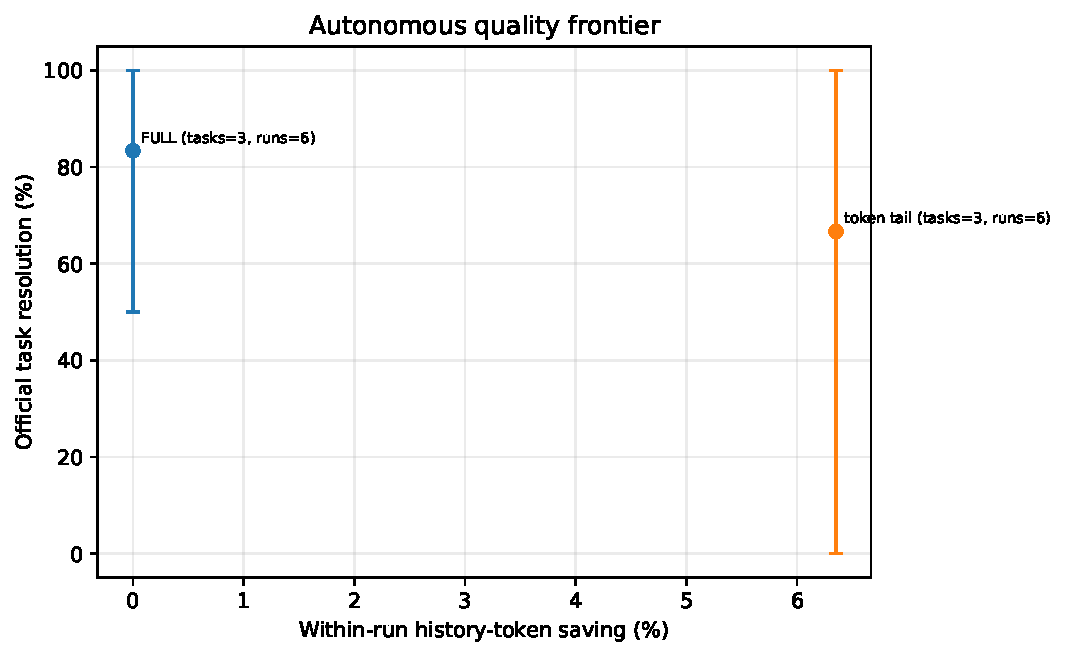
\includegraphics[width=.72\linewidth]{../shared/results/paper8_5_agent_memory/autonomous_nondominated_tail95_v1/qualified_three_task_curves/autonomous_saving_vs_accuracy.pdf}
\caption{The first autonomous accuracy--saving point. Error bars are
task-clustered and necessarily wide for three identities. The tail policy is
not promoted because its point lies below the predeclared quality gate.}
\label{fig:tail95-qualified-curve}
\end{figure}

The Task 5 failure is mechanistically informative. Both treatment repeats are
exact 19-call reproductions. They make the intended one-line source edit and
inspect its unified diff, but the completion command emits a nearby source
excerpt after the submission sentinel. The official harness therefore records
\texttt{Patch Apply Failed}. The original task and submission instructions are
still pinned, so this is not simple task-statement loss. A frozen terminal
counterfactual also restores the complete history and reproduces exactly the
same invalid command; no omitted terminal bundle can repair the already-formed
path. The first repeat-qualified materialization effect occurs at decision 3,
where shortening a 5,757-token source observation to 5,468 tokens changes the
exact reproduction command but preserves its diagnostic intent. Causal
attribution of the later submission failure therefore requires a
snapshot-restored rollout from that frontier, not terminal add-back. It also
motivates a task-aware progress spine that protects mutation, verification,
and submission state. The ungraded workspace is not counted as successful
auxiliary evidence.

The campaign also tightened the evidence machinery. Exact pre-report patch
failures and empty submissions are now definitive primary failures; a resident
grader image is reused only after architecture inspection; and sparse request
indices are rejected. One paused FULL solve has indices 1--11 and 13--22 and
is preserved but excluded rather than silently renumbered. The raw runs,
qualification decision, curves, and reductions are in
\path{autonomous_nondominated_tail95_v1}.

\subsection{Submission-guarded matched tail-90 bridge}

\paragraph{Post-refactor selector audit.}
Re-reduction of the immutable artifacts reproduces every published total
below, so the reducer refactor did not change the measurements.  The audit did,
however, expose an older implementation defect: the matched-tail manifests
recorded protected head/tail parameters, but the materializer ignored them.
The historical mini-swe-agent and OpenHands rows therefore remain valid for the
\emph{actual} prompt-pinned pure-recency policy that ran, not for H2/T4.  We
label them legacy results and require fresh corrected H2/T4 executions before
using that policy name or promoting a default.  The corrected implementation
passes the complete Paper~8.5 regression suite and records floor overflow
explicitly rather than silently retiring a protected turn.

The tail-95 stop exposed a protocol confound: mini-swe-agent accepted any
terminal payload after its completion sentinel, even when that payload was
source context rather than a unified diff. We therefore added a structural
unified-diff validator. A malformed terminal payload is now returned as a
recoverable nonzero observation; it is never replaced silently by the
workspace diff. We then reran Tasks 1--3 with two fresh \textsc{Full}
controls and a matched token-tail arm at a nominal 90\% ceiling. All runs use
mini-swe-agent 2.4.6, the observed Qwen3-Coder-30B digest, the corresponding
tokenizer, temperature zero, and immutable Docker image identities.

\begin{table}[H]
\centering
\scriptsize
\caption{Submission-guarded mini-swe-agent legacy pure-tail-90 bridge. Own M
is materialized saving on the candidate trajectory; paired M uses the predeclared
FULL-A workload. The historical manifests' H2/T4 label is superseded.}
\label{tab:mini-guarded-tail90}
\begin{tabular}{lrrrrrr}
\toprule
Task & FULL-A & FULL-B & Tail & Calls A/B/T & Own M & Paired M \\
\midrule
\texttt{django-15277} & 1 & 1 & 1 & 24/27/27 & 12.93\% & $-25.95$\% \\
\texttt{django-15368} & 1 & 1 & 1 & 15/21/16 & 13.10\% & 0.24\% \\
\texttt{scikit-learn-13135} & 1 & 1 & 1 & 23/21/19 & 9.67\% & 32.13\% \\
\midrule
Pooled workload & 3 & 3 & 3 & 62/69/62 & 11.68\% & 9.38\% \\
\bottomrule
\end{tabular}
\end{table}

Thus the legacy selective arm preserves 3/3 official resolutions and matches
FULL-A's 62 aggregate calls. It materializes 337,133 of 381,737 tokens on its
own trajectories, and 337,133 versus 372,032 tokens in the predeclared paired
comparison. Whole-causal-group selection retains 348,364 tokens, for 8.74\%
own logical saving; natural-boundary record-internal spans raise materialized
saving to 11.68\%. This passes the no-loss and no-aggregate-call-increase gates, but
it remains far below the 30--50\% saving objective.

The duplicate controls are essential. Their call counts differ by 3, 6, and
2 even at temperature zero. On Task 1 the selective trajectory's first
assistant-action divergence occurs at action 2, before the first selection
change at request 3; its negative paired value therefore cannot be assigned
cleanly to selection. We retain both the strict FULL-A pairing and the
FULL-repeat envelope instead of choosing the more favorable control after the
fact. Evidence and task-clustered curves are in
\path{cross_agent_transfer/mini_swe_guarded_tail90_three_task_v2}.

Fresh corrected H2/T4 execution resolves all three tasks.  Calls are
23/15/23 for FULL-A, 27/21/21 for FULL-B, and 20/22/22 for the candidate.
Candidate materialized own savings are 9.35\%, 8.11\%, and 7.62\%; paired savings versus
FULL-A are 22.88\%, $-48.93$\%, and 14.27\%.  The pooled 8.17\% own and 6.28\%
paired materialized savings come with three additional calls versus FULL-A,
while pooled whole-group logical saving is 6.03\%.  Thus the arm does
not pass the efficiency gate.  A second corrected Task~1 execution resolves in
26 calls at 11.28\% own saving.  Its first fork from FULL-A precedes the first
selection change by six actions, preventing attribution of its longer
trajectory to selection alone.  Evidence is in
\path{cross_agent_transfer/mini_swe_corrected_h2t4_three_task_v3}.

The first corrected OpenHands transfer uses the identical H2/T4 policy on
Task~1.  It resolves officially with the exact successful 689-byte patch
digest, reduces actions from 33 to 31, saves 35.35\% against its own trajectory,
and saves 43.53\% against paired \textsc{Full}.  Unlike the mini-swe cohort,
the richer history contains an oversized early source view, so whole-turn
retirement produces material headroom.  This is evidence for portability of
the logical abstraction, not yet for cross-agent accuracy: it is one identity
and one selective execution.  The immutable decision record is in
\path{cross_agent_transfer/openhands_corrected_h2t4_task01_v3}.

The first exact Pi treatment is a negative transfer on the same Task~1 and
Qwen3-Coder-30B endpoint.  Its fresh \textsc{Full} control resolves in 28 model
calls with the minimal 689-byte patch.  The treatment also stops after 28
calls, but fails officially with a 91,283-byte patch that removes 2,443 source
lines.  Own-trajectory whole-group saving is only 0.30\%; record-internal
ordinary-text materialization raises the apparent value to 8.53\%, and paired
materialized saving is 8.47\%.  The two arms share seven initial tool actions.
Request~8 is the first changed materialized input and tool action; request~9
begins repeatedly tail-rewriting an older oversized source view.  Three failed
edits are followed by creation of a partial file fragment, destructive copy,
and a failed attempt to restore a nonexistent backup.  The derived base image
is clean, so this is not cross-arm workspace contamination.

This execution fails the policy gate and exposes an invalid runtime mapping:
post-hoc text rewriting cannot be counted as resident K/V omission.  The
replacement frozen contract permits internal selection only when natural
child spans, completeness, and stable identity were declared before the
original K/V was encoded.  Otherwise only whole-record retirement is eligible.
Evidence and the first-divergence audit are in
\path{cross_agent_transfer/pi_exact_h2t4_task01_v3}; the replacement contract
is \path{configs/cross_agent_model_replication_v2.json}.

Two declared-safe repeats then isolate the repair from policy utility.  Both
H2/T4 and H2/T8 preserve the official solve and exact minimal patch without
rewriting any selected record.  H2/T8 is the less costly arm: 39 versus 28
FULL calls, 41.53\% own whole-record saving, and 11.81\% paired saving.  It
still fails promotion because the extra recovery calls consume most of the
omission benefit.  The compact evidence bundle is
\path{cross_agent_transfer/pi_declared_safe_task01_v4}.

\section{Detailed Transfer Protocol}

\subsection{Second open-source harness}

After policy qualification on mini-swe-agent, we transfer only the top policies
to other agents on the same ordered Easy-14 cohort.  Pi is the first admission
target because its native file, search, edit, write, and Bash operations expose
standard tool-call/result identity with little hidden orchestration.  Kilo is
the second same-model open-source admission; OpenCode is the third typed-tool
transfer; and PRA Agent is the required
record-native transfer.  OpenHands is the supplementary richer-tool transfer;
we use the current SDK directly, disable its condenser, and inventory its
runtime state rather than relying on the unmaintained standalone CLI.  The goal is not a
second exhaustive grid or an agent leaderboard, but to test whether
semantic-role findings generalize when the harness has richer tools and memory
processing.

Every agent first runs \textsc{Full}.  Policies are evaluated only on task
identities that the same agent solves under that control.  We report both the
unconditional resolution rate over all 14 identities and conditional
preservation on the agent-specific \textsc{Full}-success subset.  Exact action
strings are not compared across different agents; the portable units are
official resolution, cumulative logical input tokens, normalized causal
actions, reacquisition, and calls to solution.  Native context compaction is
disabled when possible and otherwise labels the arm as agent-managed context.

The current declaration and staged gates are in
\path{configs/agent_transfer_easy14_v2.json}; the v1 file remains the immutable
pre-131K campaign snapshot.  Across agents, only native-event
normalization, declared tool semantics, and protocol-valid serialization may
change.  Instruction pinning, causal-group atomicity, progress-spine floors,
retirement parameters, and token accounting remain frozen.  Standard OpenAI
tool traffic is recordized directly; the compatibility layer preserves
\texttt{tool\_calls}, \texttt{tool\_call\_id}, and multi-call causal groups rather
than projecting them into mini-swe-agent's assistant/user Bash convention.

OpenCode 1.18.31 uses the same transverse path rather than a distinct memory
policy.  Its thin runner invokes the official headless
\texttt{run --format json} interface, pins both the primary and small model to
the controlled checkpoint, disables native auto-compaction and external
plugins, and feeds typed tool events through the same canonical reducer used by
Kilo.  Native Bash remains an unknown-effect barrier; read, glob, grep, edit,
write, progress, and delegation tools receive declarative semantics in
\path{configs/opencode_tool_semantics_v1.json}.  A nested \texttt{task} call
fails root-trace qualification until child-session events are joined.  The
implementation is complete, but no OpenCode quality or saving number is
reported before its same-model \textsc{Full} admission succeeds.  The pinned
Linux/amd64 image and hermetic configuration pass preflight on the Medium Mac:
the CLI reports version 1.18.31 and exposes only
\texttt{pra/qwen3-coder:30b}.  This installation evidence is archived in
\path{cross_agent_transfer/opencode_admission_preflight_v1}; it is not a task
or policy result.

A later control audit found that model pinning alone was insufficient:
OpenCode applies a model-specific sampling default, documented as typically
0.55 for Qwen when the agent temperature is absent.\footnote{OpenCode agent
configuration, \url{https://opencode.ai/docs/agents/}.} The admission config now
freezes temperature 0, top-$p$ 1, and seed 0 inside the selected
\texttt{build} agent, and the runner rejects a config that omits or changes any
of those values.  Delegation is disabled for the first admission so the root
event stream is complete; child-session joining remains a separate future
qualification.  This repair invalidates no reported task result because the
model-backed OpenCode control had not yet run.

\subsection{First Pi admission outcome}

The first exact-parameter control uses Pi 0.75.3 on
\texttt{django\_\_django-15368}.  All 22 requests preserve the complete native
message sequence, standard tool identities, and fixed generation parameters
(temperature 0, top-$p$ 1, seed 0, and a 1,024-token completion ceiling).  Pi
produces the minimal one-line source fix in 22 model calls and 21 native tool
calls.  The official SWE-bench report resolves the task: 1/1
FAIL\_TO\_PASS and 29/29 PASS\_TO\_PASS tests pass.

This control exposes two transfer requirements before any savings claim.
First, six tool results are errors, including invalid edit schemas and failed
environment probes; the failed action, error result, and recovery must remain
an atomic causal group.  Second, Pi reports 419,139 cumulative logical input
tokens including its system prompt and tool schemas.  Those bytes are absent
from the existing mini-swe message-content counter, so raw token totals cannot
be pooled across agents.  Savings are paired within agent, while official
resolution and normalized actions are the portable outcomes.  The compact
decision record and complete request audit are in
\path{cross_agent_transfer/pi_task02_full_controlled_v1}.  One solved control
admits Pi to the three-task ladder; it does not estimate transfer accuracy or
qualify a policy.

The second staged \textsc{Full} control, Django-15277, also resolves
officially: both 2/2 FAIL\_TO\_PASS and all 158/158 PASS\_TO\_PASS tests pass.
Pi uses 23 model calls and 22 native tool calls, with 403,543 cumulative logical
input tokens and 2,560 output tokens.  The final source change is the minimal
guard around \texttt{MaxLengthValidator}; an untracked temporary file is not
included in the submitted patch.  Three native \texttt{edit} attempts fail
before a Bash recovery succeeds, reinforcing that action, semantic failure,
and recovery are one atomic unit.  Evidence is in
\path{cross_agent_transfer/pi_task01_full_controlled_v1}.

The third plain control, \texttt{django\_\_django-15741}, fails \textsc{Full}
for an agent-loop reason rather than selection.  After seven model calls and
six tools, the final response reaches the 1,024-token completion ceiling while
stating the correct \texttt{str(format\_type)} direction but before issuing a
write.  Pi treats the length-stopped reasoning-only response as terminal and
exports an empty patch.  Thus Pi completes the plain-three ladder with two
official successes; only Tasks 1 and 2 enter its policy-pairing denominator.
The result adds a portability invariant: provider transport termination,
including \texttt{finish\_reason=length}, is not semantic agent completion.
A separately declared 2,048-token diagnostic passes the seventh call but still
fails after 14 calls and ten tools.  It creates only an untracked reproduction
script, then performs three automatic retries after streamed responses end
without a finish reason; the final tracked patch is again empty.  Thus raising
the ceiling alone does not recover capability: agent-loop continuation and
provider stream termination both require qualification.  The diagnostic cannot
replace the frozen control.  Evidence is in
\path{cross_agent_transfer/pi_task04_full_controlled_v1}.

\subsection{First Kilo admission outcome}

Kilo 7.7.5 independently solves the same locked task with the identical
one-line patch.  Its 23 audited model requests contain 22 native tool calls
(nine reads, five greps, four Bash calls, three globs, and one edit), and the
official grader again passes 1/1 FAIL\_TO\_PASS and 29/29 PASS\_TO\_PASS tests.
The run reports 391,091 cumulative logical input tokens, but, as for Pi, this
includes the agent's own prompt and tool schemas and is used only for
within-Kilo pairing.

Kilo exposes a second normalization requirement.  All tool events carry a
transport status of \texttt{completed}, while four outputs contain failure
signals, including a missing test runner, a missing entry point, and a Python
traceback.  Portable memory policy cannot infer semantic success from transport
completion: runtime metadata should carry exit status and structured failure
evidence when the agent does not.  The admission evidence is in
\path{cross_agent_transfer/kilo_task02_full_controlled_v1}.  Like the Pi row,
this admits a harness to the staged ladder but does not qualify any retention
policy.

The second controlled success, \texttt{django\_\_django-15277}, produces the
same minimal guarded \texttt{MaxLengthValidator} patch and passes 2/2
FAIL\_TO\_PASS plus 158/158 PASS\_TO\_PASS tests.  It requires 17 model
calls and 16 native tools, with 289,550 cumulative logical input tokens and
1,425 output tokens.  Four tool outputs contain semantic failure signals even
though their transport status is \texttt{completed}, independently confirming
that transport and semantic success require separate fields.  Evidence is in
\path{cross_agent_transfer/kilo_task01_full_controlled_v1}.

A fresh exact-pair audit exposes a Kilo-specific source of false mismatch:
the harness appends a wall-clock \texttt{Message time} to its environment
block.  We normalize only this declared volatile field to a fixed string in
both arms.  The normalized Full and declared-safe H2/T4 requests then share
the exact initial SHA-256 digest and generation controls.  Both executions
resolve and produce the same minimal 689-byte patch, using 20 and 19 proxy
requests respectively.  However, their first canonical tool actions already
differ, while record selection does not activate until request~8.  The
candidate's 7.30\% own saving is valid, but its $-158.18$\% paired saving is
not causally attributable to selection.  This is a strict negative promotion
result and evidence that a temperature-zero pair still requires a
preselection-divergence audit.  The compact ledger is in
\path{cross_agent_transfer/kilo_declared_safe_task01_v2}.

The third plain control, \texttt{django\_\_django-15741}, is a genuine
\textsc{Full} failure after a hermetic retry.  Disabling external telemetry,
default plugins, project configuration, and persistent session storage removes
an earlier TLS stall.  The clean execution makes 13 model calls and 12 tools,
correctly localizes the lazy-string bug, then reaches the 1,024-token completion
ceiling while describing the edit but before issuing a write.  Kilo terminates
on that provider stop and exports an empty patch.  It therefore completes the
plain-three ladder at 2/3; only Tasks 1 and 2 enter policy pairing.  This is a
second independent example of why provider termination is not semantic agent
completion.  Evidence is in
\path{cross_agent_transfer/kilo_task04_full_controlled_v1}.

\subsection{OpenHands admission outcomes}

OpenHands SDK 1.49.2 provides the richer-tool supplementary transfer.  We run
the SDK directly inside the official task-derived container with its native
terminal, file-editor, task-tracker, think, and finish actions; the deprecated
standalone CLI and the Agent Server workspace layer are not required.  The SDK
condenser is explicitly \texttt{None}, so an agent-native summary cannot be
mistaken for PRA selection.

The first clean \textsc{Full} control, \texttt{django\_\_django-15277}, contains
33 contiguous model requests, all exact pass-through at 100\% retention.  It
produces the same minimal 689-byte guarded \texttt{MaxLengthValidator} patch
and officially passes 2/2 FAIL\_TO\_PASS plus 158/158 PASS\_TO\_PASS tests.
It consumes 641,509 cumulative provider prompt tokens and 5,747 completion
tokens.  Its 33 native actions comprise 18 terminal, 13 file-editor, one think,
and one finish action; four observations carry semantic failure evidence.
These totals include the OpenHands system prompt and tool schemas and are valid
only for within-agent pairing.

Admission exposed an SDK accounting defect before the first action.  OpenHands
assumed an optional Anthropic-style \texttt{cache\_creation\_tokens} field was
present on every OpenAI-compatible usage wrapper and aborted a valid Ollama
completion.  The compatibility guard zero-defaults only that absent telemetry
bucket; it does not modify requests, responses, tools, or selection.  External
telemetry is disabled for the hermetic retry.  An earlier post-fix diagnostic
also reaches the identical source patch but takes 35 rather than 33 actions;
assistant content first diverges at decision 22 despite temperature zero.
Official resolution, not exact cross-repeat trajectory identity, remains the
primary endpoint.

This agent also changes the portable metadata contract.  Repeated task-tracker
updates are versions of one durable logical resource rather than unrelated
text records, so the generic declaration assigns them the stable
\texttt{agent://task-tracker} identity.  File-editor commands expose their
operation and path through argument-based semantics.  Arbitrary terminal
commands remain unknown-effect barriers unless middleware supplies complete
resource/effect receipts.  Evidence is in
\path{cross_agent_transfer/openhands_task01_full_controlled_v1}.  A frozen
event-to-receipt smoke pairs all 33 actions with observations and represents
the four nonzero/error outcomes as semantic failures despite successful
transport.  It marks 32 results complete, but certifies complete effects for
only the two non-workspace control operations.  The other 31 terminal/editor
records remain fail-closed barriers because this historical execution did not
capture before/after filesystem versions.  Thus event normalization is
qualified, while resource tracing is still required before DAG retirement.

A prospective \textsc{Full} receipt run then exercises the generic side channel
inside the live task container.  All 27 model requests succeed, and all 27
native action--observation pairs emit and deliver one receipt; the proxy joins
all 26 receipts that precede a later generation.  The finalization receipt has
no later request by construction.  Nine file-editor actions carry exact
before/after file versions, while all 16 generic terminal actions correctly
remain unknown-effect barriers.  Twenty-six results are complete, 11 effect
scopes are complete, and one observation is a semantic failure.  The run
produces the same 689-byte patch as the independently graded control, although
we do not count patch identity as a second official resolution observation.
Evidence is in
\path{cross_agent_transfer/openhands_task01_full_receipt_smoke_v1}.

This prospective smoke found one adapter regression: the side-channel receipt
contained the file versions, but canonical DAG metadata did not mirror them
into the existing pre/post version maps.  The corrected bridge and regression
test now preserve those versions.  Because this run retained full history, the
defect changed neither selection nor output.

The post-fix prospective control then reproduces the earlier 33-action
trajectory, including 641,509 prompt tokens, 5,747 completion tokens, and the
same patch.  All 33 model requests and receipt deliveries succeed.  At the last
generation the canonical recordizer sees 13 versioned file-editor observations;
the 18 generic terminal actions remain conservative barriers.  The independent
official grader again passes 2/2 FAIL\_TO\_PASS and 158/158 PASS\_TO\_PASS tests.
This qualifies live receipt joining and file-editor version propagation at
full retention, but not a selective policy or arbitrary-shell retirement.
Evidence is in
\path{cross_agent_transfer/openhands_task01_full_receipt_postfix_v1}.  The staged
result demonstrates why transport success, semantic status, result completeness,
effect completeness, resource versions, and task quality must remain separate.

A second predeclared control, \texttt{django\_\_django-15368}, also resolves.
It finishes normally after 38 actions and receipts, materializes 153,174
cumulative message-content tokens, and reports 548,704 provider prompt tokens
plus 5,986 completion tokens.  The official grader passes 1/1
FAIL\_TO\_PASS and 29/29 PASS\_TO\_PASS tests.  The submitted 671-byte patch
changes the expression guard in \texttt{bulk\_update}; 21 generic terminal
actions remain barriers and 14 file-editor observations expose versioned
resources by the last generation.  Evidence is in
\path{cross_agent_transfer/openhands_task02_full_receipt_pinned_transport_v1}.

This control also exposed a transport confound that must not be attributed to
selection.  OpenHands' implicit request timeout began overlapping retries
during one long full-history generation.  We quarantine that attempt, then
pin a 1,200-second request timeout and zero automatic retries.  The corrected
run completes all 38 requests without a transport failure.  Request timeout
and retry policy are therefore part of the agent execution fingerprint; an
automatic retry is not a new semantic decision and cannot be counted as an
ordinary policy-induced call.

The third control, \texttt{django\_\_django-15741}, finishes normally after 43
actions and receipts.  It materializes 227,056 cumulative message-content
tokens; provider accounting reports 812,507 prompt and 7,130 completion
tokens.  Its 1,049-byte patch passes 2/2 FAIL\_TO\_PASS and 104/104
PASS\_TO\_PASS tests.  Twenty-seven terminal actions remain barriers, while
14 file observations expose versions by the last generation.  Evidence is in
\path{cross_agent_transfer/openhands_task04_full_receipt_pinned_transport_v1}.

OpenHands therefore completes its predeclared plain-three admission at 3/3
official resolutions.  All three identities may enter paired policy
evaluation; no \textsc{Full} result by itself qualifies a retention policy.

We next apply the same legacy prompt-pinned causal token-tail arm at a nominal 90\%
materialized-token ceiling.  Table~\ref{tab:openhands-tail90} reports the first
prospective cross-agent policy cohort.  All three selective executions resolve
officially, and each uses fewer actions than its paired \textsc{Full} control.
The pooled candidate materializes 302,487 message-content tokens rather than
569,175 for the paired controls, a 46.86\% paired saving, while actions fall
from 114 to 79.  Within the candidate trajectories alone, materialization
saves 22.49\%; the larger paired figure includes beneficial trajectory
contraction and is therefore not interchangeable with selector efficiency.

\begin{table}[H]
\centering
\scriptsize
\caption{OpenHands legacy pure-tail transfer. Own savings use each candidate's
unmodified trajectory as denominator; paired saving uses the corresponding
\textsc{Full} workload. L/M separate logical whole-record retirement from
ordinary-text materialization. All resolution cells are official; the
historical manifests' H2/T4 label is superseded.}
\label{tab:openhands-tail90}
\begin{tabular}{lrrrrrr}
\toprule
Task & FULL & Tail & Calls F/T & Own L & Own M & Paired M \\
\midrule
\texttt{django-15277} & 1 & 1 & 33/24 & 42.53\% & 42.53\% & 55.06\% \\
\texttt{django-15368} & 1 & 1 & 38/33 & 10.88\% & 10.88\% & 13.54\% \\
\texttt{django-15741} & 1 & 1 & 43/22 & 1.94\% & 9.33\% & 62.51\% \\
\midrule
Pooled workload & 3 & 3 & 114/79 & 20.71\% & 22.49\% & 46.86\% \\
\bottomrule
\end{tabular}
\end{table}

The nominal 90\% value is a strict ceiling, not a promise to retain exactly
90\%.  Complete causal turns can leave budget unused: Task 1 reaches as low as
42.61\% realized logical retention.  Conversely, Task 4 selects 98.33\% of
logical source tokens on its final request but materializes 90.02\% by slicing
an oversized observation at a natural boundary.  That distinction defines the
engine-transfer contract.  Paper 4.5 may count only selected original K/V
cells; it may not credit the additional ordinary-text compaction unless the
engine supports original-position record-internal K/V spans without
re-encoding.  Provider prompt-plus-completion accounting independently falls
45.08\% over the cohort, but remains an agent-specific secondary measure.

This three-task point meets the exploratory 30--50\% paired-saving gate with
zero observed resolution loss and no aggregate call increase.  It does not
justify a production default: there is one selective execution per identity,
one agent, and one model family, and the task effects are heterogeneous.  The
immutable reduction is in
\path{cross_agent_transfer/openhands_matched_tail90_three_task_v1}; each sibling
task directory contains native events, request traces, and official reports.

This row is not yet a quantitative mini-swe-agent versus OpenHands comparison.
Although both use the pinned Qwen3-Coder-30B checkpoint, the existing
mini-swe-agent confirmation used a 95\% tail on a partly different task cohort,
whereas this OpenHands row uses the 90\% arm above.  We therefore treat the
OpenHands result as policy-transfer evidence and require the locked Tasks
1/2/4, tail-90 pair on mini-swe-agent before estimating an agent effect.
Furthermore, the historical OpenHands proxy trace records
\texttt{whitespace\_v1\_diagnostic} token accounting rather than the pinned
Qwen tokenizer and its manifest does not bind the endpoint model digest.  Its
3/3 official quality outcome remains valid and its paired workload reduction
is a within-agent diagnostic, but 46.86\% is not an exact cross-agent token
comparison.  At that stage, strict transfer required fresh Full/tail-90 runs for both agents
with the exact Qwen tokenizer revision and endpoint digest recorded.  Prior
rows using Qwen2.5-Coder-14B or 7B remain model-specific diagnostics and are
not pooled with either arm.

That strict legacy-policy transfer is complete on the common Tasks~1--3 cohort.
Table~\ref{tab:openhands-exact-tail90} supersedes the historical whitespace
token accounting for quantitative use.  All six arms bind the observed
\texttt{qwen3-coder:30b} digest, its exact tokenizer revision, temperature
zero, the task-derived workspace image, disabled native condensation, and
zero semantic-request retries.  The actual policy is matched token-tail at a
nominal 90\% budget with immutable prompts and a contiguous causal recency
tail.  The recorded two-head/four-tail parameters were not consumed and are
not part of this result.

\begin{table}[H]
\centering
\scriptsize
\caption{Exact-token OpenHands legacy pure-tail transfer on the locked
Tasks~1--3 cohort.
Own L/M separates whole-causal-group logical retirement from record-internal
materialization; paired M includes trajectory-length effects.
Every resolution cell is from the independent official grader.}
\label{tab:openhands-exact-tail90}
\begin{tabular}{lrrrrr}
\toprule
Task & FULL & Tail & Actions F/T & Own L/M & Paired M \\
\midrule
\texttt{django-15277} & 1 & 1 & 33/24 & 54.08/54.08\% & 63.26\% \\
\texttt{django-15368} & 1 & 1 & 38/21 & 6.05/9.66\% & 39.11\% \\
\texttt{scikit-learn-13135} & 1 & 1 & 20/19 & 1.21/9.57\% & 10.15\% \\
\midrule
Pooled workload & 3 & 3 & 91/64 & 26.52/29.82\% & 43.58\% \\
\bottomrule
\end{tabular}
\end{table}

The candidate selects 658,833 of 896,615 tokens as whole causal groups and
materializes 629,228 after natural-boundary subdivision, giving 26.52\%
logical and 29.82\% materialized own saving.  It materializes those 629,228
tokens versus 1,115,305 for paired \textsc{Full}; provider prompt accounting
falls 39.90\%.  Thus the cohort reaches the exploratory 30--50\% paired
workload target with no observed quality loss or aggregate action increase.
The task-clustered mean paired saving is 37.51\%, and the wide
10.15--63.26\% range is scientifically important: the same policy has little
to retire on the short Scikit-learn trajectory but contracts the longer
Django trajectories substantially.  One run per OpenHands arm is still too
small for a production-default accuracy claim.

The submission-guarded mini-swe-agent cohort uses the same three task
identities, model digest, exact tokenizer, sampling controls, and audited
legacy pure-tail policy.  It preserves 3/3 official resolutions with
8.74/11.68\% logical/materialized own and 9.38\% paired materialized saving,
and 62 versus 62 calls.  OpenHands preserves 3/3 with 26.52/29.82\%
logical/materialized own and 43.58\% paired materialized saving and 91 versus
64 actions.  The logical policy is
engine independent, but opportunity is workload dependent: OpenHands carries
richer schemas and larger observations, and its selective trajectories
contract more.  Repeat controls are required before assigning the complete
cross-agent gap causally to selection rather than backend trajectory variance.

Admission also found a wire-compatibility failure that invalidated the first
Task~2 \textsc{Full} attempt.  This Ollama OpenAI endpoint ignored
\texttt{max\_completion\_tokens}; a declared 1,024-token request generated
more than 12,000 tokens before cancellation.  A direct four-token diagnostic
reproduces the defect, whereas \texttt{max\_tokens=4} stops at exactly four
tokens.  The proxy now validates the logical limit, normalizes it to the
portable wire key, and audits reported usage for overshoot.  The invalid run
is quarantined and absent from every aggregate.  The runner additionally
performs a bounded Docker-network preflight before the first semantic request.
Evidence is in
\path{cross_agent_transfer/ollama_completion_limit_wire_compatibility_v1},
the three \path{openhands_task0*_exact_tail90_h2t4_v2} directories, and
\path{cross_agent_transfer/openhands_exact_tail90_three_task_v2}.

\subsection{Codex Responses admission}

Codex CLI is a distinct transport case because it speaks the Responses API
rather than Chat Completions.  We therefore implement a hermetic task-derived
runner and a \textsc{Full}-only audit proxy that preserves the native wire
protocol, fills the frozen sampling controls when the CLI omits them, and
records whether later turns carry complete input or provider-managed
\texttt{previous\_response\_id} state.  No memory-policy result is claimed
until this inventory is complete: applying the Chat-Completions recordizer to
a Responses session without proving state ownership would conflate agent
transfer with a transport rewrite.  The first Task-1 control remains pending.

For the open-model cohort we additionally enable Codex's native
\texttt{--oss --local-provider ollama} mode.  Codex therefore owns the Ollama
adaptation, and no external Responses-to-Chat translation is attributed to
PRA.  The Responses audit mode remains available as a separately labelled
transport study; its state semantics cannot be pooled with the native Ollama
admission.  Native admission now fails closed unless the Ollama catalog exposes
the exact declared model digest.  Codex CLI 0.153.0 does not expose native
Ollama temperature, top-$p$, or seed controls, however, so that arm records
sampling as agent-native and unverified rather than falsely labeling it a
temperature-zero comparison.  It may establish capability and protocol shape;
it cannot enter the strict frozen-sampling agent comparison until request-side
sampling is observed or controlled.

\subsection{PRA Agent}

The final transfer uses PRA Agent, where typed task, tool, result, progress, and
subagent records are native objects. This tests whether a record-native agent can
exploit the same policy more cleanly than a retrofitted linear-message harness.
The existing generic campaign runner admits only synthetic fixtures, so we add
a SWE-bench adapter whose host-side typed tools execute inside the official task
container and export the patch to the common grader.  During admission work we
also found a transport defect: an ordinary OpenAI endpoint returning native
\texttt{tool\_calls} with null text became the literal answer \texttt{None},
terminating the agent before its first action.  The transport now losslessly
projects native calls into the agent executor's provider-neutral envelope and
records cumulative provider usage.  This is an implementation qualification,
not by itself a policy result.

The corrected \textsc{Full} admission resolves
\texttt{django\_\_django-15368} with the same minimal 671-byte patch as Pi and
Kilo: the official grader passes 1/1 FAIL\_TO\_PASS and 29/29 PASS\_TO\_PASS
tests.  PRA Agent requires nine model requests and eight typed tool executions,
with 86,626 cumulative prompt tokens, 16,353 cached prompt tokens, and 1,356
completion tokens.  The run exposed three further portability invariants.
Transient provider control tokens must not be replayed as ordinary assistant
text; intermediate assistant actions and arguments must be durable causal
records; and a tool-handler exception must become a typed failure observation
rather than terminate the agent.  The complete session and grading evidence
are in \path{cross_agent_transfer/pra_agent_task02_full_controlled_v1}.  As for
the other admissions, this single task opens the staged three-task ladder but
does not estimate policy accuracy.

The second controlled admission, \texttt{django\_\_django-15277}, exposes a
different provider boundary.  After nine valid typed actions, the model emits
its next \texttt{search\_text} decision using PRA Agent's exact durable textual
projection rather than a native \texttt{tool\_calls} object.  The pre-fix loop
mistakes that action for a final answer and exports an empty patch.  We accept
the serialized representation only when the PRA-owned action sentence
terminates the response; ordinary prose and quoted examples remain
non-executable, and disclosure, schema, and authorization checks are
unchanged.  The corrected retry reaches the exact minimal source fix in 14
model requests and 13 typed tool executions.  The official instance report
passes 2/2 FAIL\_TO\_PASS and 158/158 PASS\_TO\_PASS tests.  It reports 125,952
cumulative prompt tokens, including 27,362 cached tokens, and 1,725 completion
tokens.  Evidence, including the quarantined empty-patch diagnostic, is in
\path{cross_agent_transfer/pra_agent_task01_full_controlled_v1}.

A later wire audit supersedes that execution for controlled comparisons.  The
remote backend forwarded the completion ceiling but omitted temperature,
top-$p$, and seed, so the server used temperature 1.0 despite the campaign's
temperature-zero declaration.  The repaired transport carries these ordinary
OpenAI fields losslessly and rejects attempts to override the request
envelope.  A fresh Task~1 \textsc{Full} control with server-confirmed
temperature 0, top-$p$ 1, and seed 0 again resolves officially with the same
689-byte patch.  It uses 15 model requests and 14 typed tools, with 148,225
cumulative prompt tokens, 30,731 cached prompt tokens, and 2,245 completion
tokens.  This is the admissible Full baseline for a future selective pair;
the earlier rows remain protocol-debugging evidence only.  The compact bundle
is in \path{cross_agent_transfer/pra_agent_fixed_sampling_task01_v2}.

This result separates compatibility from memory quality.  A tool decision may
have several protocol encodings, but it crosses the execution boundary only
through an unambiguous terminal envelope.  Repairing that boundary changes
agent capability on the same \textsc{Full} history and therefore must precede,
not be credited to, any retention-policy comparison.  PRA Agent has now
resolved two plain controls.

The third control, \texttt{django\_\_django-15741}, reveals two more wire-level
variants before reaching a genuine agent outcome.  The provider first emits a
terminal Qwen \texttt{<function=...>} block rather than an OpenAI tool object;
the runtime now parses that block only when it is structurally complete and
terminal.  A later attempt contains malformed JSON.  The runtime does not
repair and execute guessed arguments: it records a visible
\texttt{malformed\_call} rejection and requests a fresh action.  Both repairs
are fail-closed and pass the same disclosure, schema, and authorization gates
as native calls.

After those compatibility repairs, the frozen \textsc{Full} control remains
unresolved.  It makes six model requests and five typed tool calls, consumes
39,491 cumulative prompt tokens (7,048 cached) and 1,584 completion tokens in
817.4 seconds, and exports an empty patch.  Its final response correctly
identifies the necessary conversion of lazy \texttt{format\_type} to a string,
then says it will implement the fix without issuing a tool action.  An earlier
diagnostic leaves an incomplete patch and fails both FAIL\_TO\_PASS tests while
passing 104/104 PASS\_TO\_PASS tests.  Thus PRA Agent completes plain-three at
2/3; only Tasks 1 and 2 enter its policy denominator.  The full controls and
quarantined diagnostics are in
\path{cross_agent_transfer/pra_agent_task04_full_controlled_v1}.

A completion-guard diagnostic then crosses that precise stopping boundary.  It
performs the source edit, exports a 793-byte patch, and the independent grader
resolves the issue.  The execution is nevertheless auxiliary rather than a new
\textsc{Full} success: after 20 successful requests, request 21 terminates with
HTTP 500 \texttt{EOF}.  The final successful response reports 32,734 prompt
tokens plus 97 completion tokens while the active Ollama runner is configured
for 32,768 tokens.  The catalog advertises the model's 262,144-token capability,
but that is not evidence of the loaded serving allocation.  We therefore add
separately digested 65,536-token single-task and 131,072-token persistent-session
serving aliases and require three identity probes, a deterministic completion,
and active-process context inspection before retry.  Evidence is in
\path{cross_agent_transfer/pra_agent_task04_completion_guard_aux_v1}.

Table~\ref{tab:same-model-task4-agent-loop} makes the causal comparison
explicit.  The rows use the same configured Qwen3-Coder-30B endpoint and task,
but not the same agent treatment.  The historical OpenHands artifact predates
digest capture, so this is a scaffold/loop diagnosis rather than a strict
bit-identical-model factorial.

\begin{table}[H]
\centering
\scriptsize
\caption{Task-4 failures under the same configured base model are explained by
agent-loop semantics, not by memory selection.  R/T is model requests or
actions / executed tools; rejected proposals are not counted as executed
tools.}
\label{tab:same-model-task4-agent-loop}
\begin{tabular}{lrrlp{4.8cm}}
\toprule
Agent & R/T & Patch & Official & Identified stopping behavior \\
\midrule
Pi & 7/6 & empty & fail & length-stopped correct reasoning treated as completion \\
Kilo & 13/12 & empty & fail & length-stopped correct reasoning treated as completion \\
PRA Agent, historical & 6/5 & empty & fail & promise to edit accepted as completion \\
PRA Agent, guarded 32K & 20/20 & 793 B & resolves$^{*}$ & edit succeeds; next request exceeds loaded 32K context \\
PRA Agent, corrected 64K & 15/12 & 701 B & resolves & host rejects two post-budget reads; model recovers and edits source \\
OpenHands & 43/43 & 1,049 B & resolves & finish requires the native completion action after mutation and verification \\
\bottomrule
\end{tabular}
\end{table}

The shared pattern is therefore identifiable: model capability was present in
all three empty-patch trajectories, but transport completion, semantic
completion, and verified workspace completion were conflated differently by
each harness.  The guarded row's asterisk denotes auxiliary patch capability,
not a qualified end-to-end control.  The corrected 64K row is a clean FULL
qualification: the independent SWE-bench grader reports one submitted, one
completed, and one resolved instance with no error.  It is not a savings row.

The final repair also exposed a subtler protocol defect.  The first bounded
inspection implementation appended ``action executed'' before the host guard
ran, then appended a user-side rejection for the same proposal.  Under this
contradictory history the model proposed four additional reads and produced no
patch.  The corrected runtime emits the executed projection only after guard
acceptance; rejected proposals instead state that they were not executed and
remain atomic with the host rejection.  On the clean retry, after eight
executed tools the host rejects two verification commands because no tracked
source mutation exists.  The model then acknowledges the constraint, edits the
named source file, simplifies the edit, inspects it, and terminates normally.
Evidence is in
\path{cross_agent_transfer/pra_agent_action_projection_audit_v1} and
\path{cross_agent_transfer/pra_agent_task04_rejection_semantics_full_v1}.

The same trace also motivates two agent-side repairs before the persistent
campaign.  Root file discovery now prunes repository-internal \texttt{.git}
state and caps its observation, while an explicitly hashed behavior contract
instructs the model to consume successful observations, avoid identical calls
unless state changed, prefer targeted reads, act rather than promise, and
verify before finalization.  These are prospective scaffold changes, not
retrospective savings.  Live PRA Agent state is atomically persisted after
each record so a host crash does not erase a long trajectory.

\subsection{Longer-horizon mini-swe-agent capability control}

We separately locked the five original Easy-50 failures whose no-PRA control
terminated at the 50-action limit.  This is a capability experiment, not a
retrospective enlargement of the Easy-14 policy cohort.  Each identity first
receives \textsc{Full} history and an 80-action ceiling; only a resolved task or
a surviving source-only patch with demonstrable forward progress may advance
to 120 actions.

The first clean execution, \texttt{sympy\_\_sympy-17655}, terminates by
submission after 60 model calls---ten beyond the original ceiling---but does
not resolve.  It consumes 946,069 cumulative logical input tokens and 15,946
reported completion tokens in 943.3 seconds.  The agent creates an intermediate
16-line source edit, later reverts it, and finally submits a prose explanation
instead of a source patch.  The official grader therefore records
\texttt{patch\_apply\_failed}.  Because no source-only patch survives at
submission, the identity fails the predeclared forward-progress gate and does
not advance to 120 calls.

The second identity, \texttt{django\_\_django-16899}, shows a different
boundary.  It stops normally after 22 model calls and 21 actions, well before
the 80-call ceiling, and submits an applicable source patch.  The run consumes
146,335 cumulative logical input tokens and 3,078 reported completion tokens
in 466.0 seconds.  However, the patch substitutes an existing helper whose
message contract is not the requested one: all 56 PASS\_TO\_PASS tests pass,
but both FAIL\_TO\_PASS tests fail.  Because no target test passes, this is a
capability error rather than a horizon-limit result and it fails the
predeclared forward-progress gate for 120 calls.  Evidence is in
\path{longer_horizon/task02_full80_v1}.

This negative control is useful: merely extending the action horizon can add
substantial repeated reading and reasoning without adding capability.  It
therefore cannot be used as a substitute for a memory policy, and a shorter
failed run cannot be credited with token saving.  The complete 60-action
history and official evidence are in
\path{longer_horizon/task01_full80_v1}.

\section{Detailed Handoff to Native Runtime Evaluation}

Paper 8.5 should freeze a small set of logical policies, for example
\[
\{\textsc{Full},\textsc{Balanced},\textsc{Aggressive}\}.
\]

A runtime study can then map the exact same \texttt{AgentMemoryPlan} to text
replay, HF cache views, MLX interval views, vLLM pages, llama.cpp resident slots,
and SGLang cache objects. The runtime study must not retune selection semantics
per engine.

Paper~8.5 reports two nested selection ledgers, not measured K/V savings.
Whole-group logical saving is the conservative lower bound that maps directly
when every causal group owns persistent original-position K/V.  Additional
record-internal materialized saving maps only when oversized observations were
pre-segmented at natural boundaries and every child span retains a stable
original K/V identity; text slicing or summary generation after caching does
not qualify.  Paired saving additionally includes trajectory contraction and
therefore predicts total workload economics, not per-request K/V omission.
Paper~4.5 must replay both ledgers unchanged and report resident K/V references,
copies, re-encoding, newly encoded suffix, temporary bytes, TTFT, and latency
separately.  It may count neither rewritten receipts nor compacted text as
resident-subset reuse.

\section{Pending Confirmatory Outcomes}

Our main hypothesis is
\[
\text{token recency}
<
\text{causal recency}
<
\text{typed progress spine + retrieval}
\]
at matched context budgets.

A positive result need not initially increase raw task success. A practically
important result is
\[
\text{same task success}
+
\text{fewer model calls}
+
\text{fewer rereads}
+
\text{fewer repeated tests}
+
\text{less retained history}.
\]

A negative result would also be informative: if simple recency performs as well
as structured policies, coding-agent memory may be more local than assumed.

\section{Detailed Limitations}

Text realization recontextualizes selected records and therefore does not
establish native-K/V equivalence.  In particular, post-cache receipt generation
must never be reported as zero-prefill resident-subset reuse merely because the
retained original records were not re-encoded. Frozen-trajectory screening also cannot replace
autonomous evaluation. SWE-bench coding tasks may not represent research,
browser, or multimodal agents. Semantic record labels may depend on heuristics
during the first implementation.

These limitations are deliberate. This paper isolates logical memory selection
before introducing engine-specific physical state. The current autonomous
controls also show that fixed temperature and seed fields do not eliminate
trajectory variation or submission failures in the tested endpoint; repeated
FULL controls and separately labelled solution-state diagnostics are needed
before attributing success or failure to a memory policy. Auxiliary workspace
grades are post-hoc diagnostics and never replace the primary agent submission.

\section{Evidence Chronology Synthesis}

Agent memory selection is a distinct problem from transformer cache reuse. A
serving engine may perfectly preserve selected native K/V while an agent policy
selects the wrong history, and a good logical policy may be obscured by an
incorrect engine implementation. We therefore study memory selection first,
using an engine-independent record interface and a minimal software-engineering
agent. The resulting policy frontier should provide a semantic contract for
later native-memory runtimes: engines realize a frozen memory plan; they do not
decide what the agent ought to remember. The first autonomous evidence further
shows that this frontier cannot be estimated from a single control trajectory:
the primary FULL submission resolves only one of two executions on each of two
task identities, even though auxiliary grading shows both FULL-B workspaces
contain resolving patches. The second task therefore fails the gate for
heuristic evaluation. H3 remains negative under both primary and auxiliary
outcomes on the first task. Within-record evidence selection provides a clearer
but still non-inert frontier: a conservative structured materializer saves
5.54\% on the repeatable 23-decision trace and preserves 54.5\% of conservative
actions, outperforming more aggressive positional materializers in agreement
but not in compression. Observation receipts now fail closed when their own
token cost is not smaller than the source and activate correctly on oversized
mechanism controls. The evidence supports a sharper hypothesis than
``semantic selection beats recency'': agent memory is not reducible to current
world state. The new three-trajectory omission oracle nevertheless finds
semantic-transition headroom of 24.5--38.2\% under bounded subset search, while
also showing that safe removals are non-additive and non-monotone. In the
deployable frozen factorial, H1+H3 whole-record retirement misses its 2\% mean
yield gate and payload receipts are low-yield or harmful. A matched recency arm
preserves all three semantic transitions at 3.0\% mean saving and is the only
candidate advanced to repeated autonomous qualification. In three same-host
task identities it saves 6.35\% of pooled treatment-history tokens, but primary
resolution falls from 5/6 FULL runs to 4/6 treatment runs. Its 66.7\%
task-macro resolution misses the 80\% gate. The repeated failure retains the
intended source edit but submits a non-patch excerpt, motivating explicit
progress/submission state rather than deeper blind recency.  The structured
observation arm supplies a more promising but still preliminary point: on one
Task-5 execution it preserves official resolution in 22 calls while saving
6.10\% of its trajectory-counterfactual materialized tokens; one of two FULL
controls resolves, and the other creates a patch but submits an empty payload.
It therefore advances to repeated multi-task confirmation, not to a profile.
The persistent N=3 campaign then provides the first profile-quality discovery
point.  Blind R4 loses both paired Scikit-learn successes; R6 is unreliable;
and R8 preserves success but saves only 13.09\% while adding calls.  A frozen
first-divergence oracle shows that this is selection-induced protocol
conditioning, not merely backend variance, and motivates one clean completed
action--observation exemplar per prior issue.  The resulting R4/M2/V2/P1 arm
resolves 6/6 issues across two executions, saves 36.41\% and 45.82\% against
paired \textsc{Full}, and reduces calls in both.  This repeated discovery result
conditionally qualifies the logical policy for frozen Paper~4.5 native-K/V
transfer when equivalent episode metadata exists, but not yet for a general
default: the uncertainty unit is still one ordered sequence family.  In the
realistic boundary-free setting, global R4 preserves all user instructions yet
resolves only 2/3, adds 11 calls, and receives zero failure-aware saving.  This
rules out treating the explicit-boundary frontier as a deployable default.  A
two-level instruction-epoch policy fixes the immediate error by keeping the
active epoch whole: its first admissible clean replication resolves 3/3 like
persistent \textsc{Full}, saves 34.83\% on the paired denominator, and uses two
fewer calls.  This qualifies sequence expansion while retaining the stronger
guardrail that dependent epochs need resource-DAG evidence.  The N=6 expansion
then rejects E0 as a deployment profile: it resolves 6/6 versus \textsc{Full}'s
5/6 and removes 55.34\% relative to its own trajectory, yet its 114 calls
consume 43.87\% more input tokens than the 60-call control.  This is the
paper's clearest demonstration that per-request pruning can lose end-to-end.
The completed E1/E2 ladder, which retains one or two recent instruction epochs
whole, rejects both repairs: E1 resolves 5/6 but adds eight calls and reaches
only 14.21\% raw paired saving; E2 uses two fewer calls and reaches 21.93\%
raw paired saving but loses a \textsc{Full} success, receiving zero
failure-aware saving in that ladder.  The frozen-prefix diagnosis reverses the
outcome: E2 resolves 2/2 and \textsc{Full} 0/2 at equal mean calls, with E2
sending 21.92\% fewer tokens.  Because byte-identical no-removal requests also
diverge at temperature zero, this is evidence of a noisy outcome surface, not
an accuracy gain.  No instruction-epoch profile transfers to Paper~4.5.
The frozen profile screen identifies E0+M1/V1/P1 at 39.81\% opportunity and
R1/M1/V1/P1 at 37.43\%, but their first autonomous pilots both fail with the
same incorrect patch.  Coarse semantic role floors therefore do not substitute
for an information-flow test.  The later recent-frontier DAG $M=2$/P1 policy
supersedes these candidates in the initial screen: it preserves 3/3 paired
successes with 40.83\% aggregate saving and no call increase.  Its first
contemporaneous Task-3 repeat preserves success and calls but saves only
9.96\%, while Task~4 repeats at 59.24\% saving and one fewer call.  This
heterogeneity fails the profile-level repeated saving gate; Task~5 additionally
has a failed contemporaneous control while M2/P1 resolves.  It therefore does not yet qualify
Easy-14 expansion or transfer as a Paper~4.5 production default.  The
one-to-fourteen-issue campaign continues to treat active-only retirement as session
hygiene unless it beats deliberate fresh sessions on related or dependent
sequences.  The PRA Agent executor records cumulative FULL-denominator and
materialized-policy tokens after every episode in one immutable fourteen-issue
session.  Thus paired FULL/selective executions yield descriptive N=1--14
prefix curves without the 105 task episodes required by separately rerunning
every prefix; those shared prefixes are not independent samples or confidence
intervals.  Held-out sequences, additional models, and additional harnesses
remain the confirmation frontier.

\section{Artifact Schema}

Each request/run should persist:
\begin{itemize}[leftmargin=*]
    \item task ID and repository revision;
    \item mini-swe-agent revision;
    \item model/tokenizer revision;
    \item generation settings;
    \item canonical trajectory digest;
    \item exact persistent-prefix digest, in-place \textsc{Full} control run ID,
    launch order, and official qualification outcome;
    \item typed record list and causal groups;
    \item selector name/revision;
    \item materializer name/revision;
    \item requested/realized budget;
    \item selected record IDs/spans;
    \item selected token count;
    \item next model response/action;
    \item primary autonomous submission result;
    \item separately labelled auxiliary final-workspace result and extraction
    availability;
    \item reread/retest/recovery counters;
    \item failure taxonomy labels.
\end{itemize}

\section{Initial Failure Taxonomy}

\begin{verbatim}
MEMORY_TASK_LOSS
MEMORY_SOURCE_LOSS
MEMORY_MUTATION_LOSS
MEMORY_VERIFICATION_LOSS
MEMORY_PROGRESS_LOSS
MEMORY_CAUSAL_PAIR_BREAK
MEMORY_STALE_HYPOTHESIS
MEMORY_REDUNDANT_REREAD
MEMORY_REDUNDANT_TEST
MEMORY_WRONG_FILE
MEMORY_REPEAT_FAILED_EDIT
MEMORY_FORMAT_REGRESSION
MEMORY_RECOVERY_SUCCESS
MEMORY_RECOVERY_FAILURE
UNQUALIFIED_SESSION_INTERFERENCE
\end{verbatim}

\bibliographystyle{plain}
% \bibliography{../shared/references}

\end{document}
